\begin{definition}[From Morse to K-Theory] \label{def:MorseFiltr:TheIdentificationChi}
	Let $M$ be a smooth manifold wit the Morse datum $\mathfrak{A}$ and denote the one point pointed space by $pt$. Then for any $l\in \N$, on the generators $\Crit_k(f)$ we define the morphism of canonical Isomorphism calses, where the left side consists of only one group:
	\begin{equation*}
		\Chi: C^k(M,\mathfrak{A},\rK^{-l}(pt))\,\to\, \rK_{\#}^{-(k+l)}(\mathcal{IP}_k)\,,\quad q\mapsto (\alpha_q^{(N_q,L_q)})_{\#}\,.
	\end{equation*}
	Remark \ref{rem:MorseFiltr-canonicalIdentificationOfMorseChainGrou} ensures invaraiance of the choosen $\epsilon$ and refined Morse chart, that made up $(\alpha_q^{(N_q,L_q)})_{\#}$.
\end{definition}

\begin{definition}[Adapted Lyapunov Function]\label{def:morseFilt-adaptedLyapunov}
	An \textbf{adapted Lyapunov function} for the Morse-Smale pair $(f,g)$ (where $g$ denotes the metric and $f$ the Morse function) is a smooth function 
	$\ell :M\to \R$ such that
	\begin{enumerate}[(i)]
		\item $\diff \ell (-\grad (f))<0$ on $M\setminus \Crit(f)$,
		\item $\ell(r)=\ind_r(f)$ for all $r\in \Crit(f)$,
		\item every $r\in \Crit(f)$ has a neighbourhood on wich $\ell-f$ is constant.
	\end{enumerate} 
\end{definition}
\begin{proposition}\label{prop:morseFiltr-existenceAdaptedLyapunov}
	An adapted Lyapunov function exists.
\end{proposition}
\begin{proof}
	We apply \cite[Theorem B]{Smale1961OnGradient} to the vector field $X=\grad(f)$, which satisfies the needed conditions: For such a setup, Smales Theorem gives us a function $F$ that satisfies
	\begin{enumerate}[(a)]
		\item The critical points of $F$ are the critical points of $X$ (and thereby, in our case of $f$) and $F$ coincides with $f+c$ for $c\in \R$ in small neigbhourhoods of those critical points,
		\item $X$ is transversal to $F$ at levelsets outside of critical points.
		\item $F(r)=\ind_f(r)$ for all $r\in \Crit(F)=\Crit(f)$.
	\end{enumerate} By (a), $\diff F(\grad(f))=\diff f (\grad(f))=\norm{\grad(f)}^2$ near critical points. Outside of critical points we have that $\diff F (-\grad(f))\neq 0$ and as for $\dim(M)\geq2$ this set is connected, we conclude that $\diff F (-\grad(f))>0$ there also. If $\dim(M)=1$ we can argue similarly in each connected component that contains a point close to a critical point. Hence, all properties of an adapted Lyapunov function are satisfied by $\ell\coloneq F$.
\end{proof}

\begin{definition}[Sublevel Index Triple]\label{def:morseFilt-sublevelTriple}
	Let 
\begin{equation*}
S_k\coloneq \Crit_k(f)\cup\Crit_{k-1}(f)\cup\bigcup_{q\in\Crit_k,\,p\in\Crit_{k-1}}W(q\to p
)\,.
\end{equation*}
	An  \textbf{index triple} for $S_k$ is a triple $Z\subseteq Y\subseteq X$ of compact sets such that $(X,Z)$ is an index pair of $S_{k}$, $(X,Y)$ is an index pair of $\Crit_{k}(f)$ and $(
	Y,Z)$ is an index pair of $\Crit_{k-1}(f)$. It is called a \textbf{sublevel triple} if moreover
	\begin{equation*}
		Y=Z\cup \big(X\cap  \ell^{-1}(-\infty,c]\big)\qquad \text{for some }c\in(k-1,k)\,.
	\end{equation*}
\end{definition}
\begin{lemma}\label{morseFiltr-sublevelTripoleGivePairs}
	Let $(X,Z)$ be an index pair of $S_{k}$, $c\in (k-1,k)$ and $Y=Z\cup \big(X\cap  \ell^{-1}(-\infty,c]\big)$. Then $(X,Y,Z)$ is a sublevel triple.
\end{lemma}
\begin{proof}
	We need to check the three axioms for the two pairs $(X,Y)$ and $(Y,Z)$. We start checking the axioms for $(X,Y)$:
	\begin{enumerate}[1.]
		\item Assume that $x\in I(\overline{X\setminus Y})$. Then $x\in I(\overline{X\setminus Z})$ and thereby $x=q$, or $x\in W(q\to p)$ for some $q\in \Crit_{k}(f)$, and $p\in \Crit_{k-1}(f)$. But the latter cannot be true, as for all $x\in W(q\to p)$, there is a $t>0$ such that $f(\phi_t(x))<c$. Hence $x=q$.
		\item Assume that $Y$ would not be positively invariant in $X$. Then there would be an $x\in \ell^{-1}(-\infty,c]$ (since $Z$ is positively invarient), and such that $f(\phi_{t}(x))>c\geq f(x)$ which cannot happen, as $f$ decreases along flow lines.
		\item Finally, as $Y$ contains $Z$, the exit set property is trivially satisfied.
	\end{enumerate}
	Now for $(Y,Z)$:
	\begin{enumerate}
		\item This is shown by the same argument as for $(X,Y)$.
		\item $Z$ is positively invariant in $X$ and $Y\subseteq X$. Hence $Z$ is positively invariant in $Y$.
		\item $Z$ is an exit set of $X$ and thereby also of $Y$, as the latter is again contained in $X$.
	\end{enumerate}
\end{proof}
\begin{lemma}\label{lem:morseFiltr-kompactImpliesTwichImpliesU}
	Let $\phi$ be a flow on $M$ (which is a locally compact metric space or in our case a smooth manifold), $K\subseteq M$ be compact and $U$ be an open set in $K$ containing the maximal invariant subset $I(K)$. Then there exists a $T>0$ with:

	\begin{equation*}
		\phi_{[-T,T]}(x)\subseteq K \qquad \Leftrightarrow\qquad x\in U
	\end{equation*}
\end{lemma}
\begin{proof}
	The contradiction would imply that for all $T$ there would be an $x$ such that $\phi_{[-T,T]}(x)\subseteq K$ but $x\notin U$. With this we define the sequence $x_n$ such that $\phi_{[-n,n]}(x_n)\in K$ but $x_n\notin U$. Now decending to a subsequence gives us a sequence $x_n$ that converges in $K\setminus U$ to a point $x$. Continuity of the flow implies that $\phi_\R(x)\subseteq K$ and hence $x\in I(K)$ which implies that $U$ was not a neighbourhood of $I(K)$. Hence, by contraposition, the original claim follows.
\end{proof}

\begin{lemma}[Flow Maps and Triples]\label{lem:morseFiltr-flowMapOfTriples}
	Let $(X,Y,Z)$ be an index triple and $(\tilde{X},\tilde{Y},\tilde{Z})$ be a sublevel triple for $S_k$, with level $\tilde{c}$. Dentote by $h_t,\,h^{k-1}_t,\, h^k_t$ the maps of Theorem \ref{thm:morseFiltr-homotopyEquivalenceOfIndexPairs} for the index pairs $(X,Z)\to (\tilde{X},\tilde{Z})$ of $S_{k}$,  $(Y,Z)\to (\tilde{Y},\tilde{Z})$ of $\{p\}$ and  $(X,Y)\to (\tilde{X},\tilde{Y})$ of $\{q\}$. Then there exists a $T_0$ such that for all $t\geq T_0$:
	\begin{enumerate}[(i)]
		\item $h_t(Y/Z)\subseteq \tilde{Y}/\tilde{Z}$,
		\item $\restr{h_t}{Y/Z}=h^{k-1}_t$,
		\item the map $X/Y \to \tilde{X}/\tilde{Y}$ induced by $h_t$ equals $h^k_t$.
	\end{enumerate}
	This means that we can view $h_t:(X/Z,Y/Z,[Z])\to (\tilde{X}/\tilde{Z},\tilde{Y}/\tilde{Z},[\tilde{Z})$ as a map of triples, such that the two diagramms (where $q$ denotes thge quotient) commute: 
	\begin{center}
		\begin{tikzcd}
			X/Y \arrow[d,"h^k_t"]&(X/Z,Y/Z)\arrow[d,"h_t"]\arrow[l,"q"]\\
			\tilde{X}\tilde{Y}   & (\tilde{X}/\tilde{Z},\tilde{Y},\tilde{Z})\arrow[l,"q"]
		\end{tikzcd}
		\qquad
				\begin{tikzcd}
			Y/Z \arrow[d,"h^{k-1}_t"]&(Y/Z,[Z])\arrow[d,"h_t"]\arrow[l,"q"]\\
			\tilde{Y}\tilde{Z}   & (\tilde{Y}/\tilde{Z},\tilde{Z})\arrow[l,"q"]
		\end{tikzcd}
	\end{center}
	
	in the first pair, it induces $h_t^k$ and in the second pair in induces $h_t^{k-1}$.
\end{lemma}
\begin{proof}
	As a reminder: For two index pairs $(N,L)$ and $(\tilde{N},\tilde{L})$, the map $h:N/L\to \tilde{N}/\tilde{L}$ is given by 
	\begin{equation*}
		([x],t) \mapsto \begin{cases}
[\phi_{3t}(x)] & \text{ if }\underbrace{ \phi_{[0,2t]}(x)\subseteq N\setminus L \text{ and } \phi_{[t,3t]}(x)\subseteq \tilde{N}\setminus \tilde{L}}_{P^{(N,l)}_{(\tilde{N},\tilde{L})}(t,x)}\\
[\tilde{L}] &\text{ else}
		\end{cases}
	\end{equation*} where $t$ is big enough. The property that gives the case destinction is denoted by $P^{(N,l)}_{(\tilde{N},\tilde{L})}(t,x)$.
	Let $x\in Y\setminus Z$ with $\phi_{[0,2t]}(x)\subseteq X\setminus Z$. The positive invariance of $Y$ in $X$ implies that $\phi_{[0,2t]}(x)\in Y\setminus Z$. By Lemma \ref{lem:morseFiltr-kompactImpliesTwichImpliesU} applied to $K\coloneq \overline{Y\setminus Z}$ with $U\coloneq \{l<\tilde{c}\}\cap K$ and $t$ big enough implies that $\phi_t(x)\in U$. Hence, $\ell(\phi_t(x))<\tilde{c}$ and as $\ell$ decreases along $\phi$, we conclude that $\ell(\phi_{[t,3t]})<\tilde{c}$. Thereby for our $x$ the conditions 
	\begin{equation*}
		\phi_{[t,3t]}(x)\in \tilde{X}\setminus \tilde{Z}\qquad\text{and}\qquad \phi_{[t,3t]}(x)\in \tilde{Y}\setminus \tilde{Z}
	\end{equation*} are equivalent, for $t$ big enough, giving us that for $x\in Y\setminus Z$, the conditions are equal: $P^{(X,Z)}_{(\tilde{X},\tilde{Z})}(t,x)=P^{(X,Z)}_{(\tilde{Y},\tilde{Z})}(t,x)$. This implies $(i)$ and also $(ii)$, as the maps are given by the same case distinctions.
	Now for the last statement: The induced map $\overline{h_t}:X/Y\to \tilde{X}/\tilde{Y}$ is well defined by $(i)$. Again, to check the equality of the induced map $\overline{h_t}$ and $h_t^q$ we go through the case destinctions in their definitions. This time, the conditions $P$ are not equivalent. And we go through the 4 possible cases: $P^{(X,Z)}_{(\tilde{X},\tilde{Z})}(t,x)$ and $P^{(X,Y)}_{(\tilde{X},\tilde{Y})}(t,x)$ are both true, are both false, or only one of them is true for $x\in X$. The first two conditions obviously give rise to the same functions. Now assume that $P^{(X,Z)}_{(\tilde{X},\tilde{Z})}(t,x)$ is true, whilst $P^{(X,Y)}_{(\tilde{X},\tilde{Y})}(t,x)$ is false. Then: 
	\begin{equation*}
		\text{either }\underbrace{\phi_{[0,2t]}(x)\begin{cases}
			\subseteq X\setminus Z\\
			\nsubseteq X\setminus Y
		\end{cases}}_{Case 1}\qquad \text{,or }
		\underbrace{\phi_{[t,3t]}(x)\begin{cases}
			\subseteq \tilde{X}\setminus \tilde{Z}\\
			\nsubseteq \tilde{X}\setminus \tilde{Y}
		\end{cases}}_{Case 2}\,.
	\end{equation*}
	Case 1: There exists a $s\leq 2t$ such that $\phi_s(x)\in Y$. Positive invariance of $Y$ in $X$ gives us that $\phi_{2t}(x)\in Y$. Now $\phi_{[t,3t]}(x)\in \tilde{X}\setminus \tilde{Z}$ gives us by Lemma \ref{lem:morseFiltr-kompactImpliesTwichImpliesU} that $\phi_t(x)$ is close to $S_{k}$, and since $q\notin Y$, we have that the number $c_0\coloneq \max\{\restr{\ell}{Y\cap S_{k}}\}<k$ Hence, by the closenes to $S_{k}$ there exists a $\delta>0$ such that $\ell(\phi_{2t}(x))<c_0+\delta<k$ for $t$ big enough. 
	On $\overline{\tilde{X}\setminus \tilde{Z}}\cap \ell^{-1}(\tilde{c},c_0)$ there critical points and hence $\ell$ is strictly decreasing. Using compactnes and the mean value theorem, we can conclude that there is a $\mu$ such that for every $x\in \overline{\tilde{X}\setminus \tilde{Z}}\cap \ell^{-1}(\tilde{c},c_0+\delta)$ and $s>0$, $\ell(x)-\ell(\phi_{s}(x))\geq \mu\cdot s$. Now we apply this idea to the intervall $[2t,3t]$ and assume that there is no $T$ big enough such that for all $t>T$, $\ell(\phi_{3t}(x))>\tilde{c}$. Then the whole curfe $\phi_{[t,3t]}(x)$ would live in $\overline{\tilde{X}\setminus \tilde{Z}}\cap \ell^{-1}(\tilde{c},c_0+\delta)$ and hence, 
	\begin{equation*}
		c_0+\delta -\tilde{c}\geq \ell(\phi_{2t}(x))-\ell(\phi_{3t}(x))\geq \mu\cdot t\,.
	\end{equation*} This cannot be true for all $t$ as the right side is unbounded in $t$ whilst the left side is constant, giving us a contradiction. Hence, for $t$ big enough $\ell(\phi_{3t}(x))<\tilde{c}$ and hence $\ell(\phi_{3t}(x))\in \tilde{Y}$. Thereby, the induced map maps such a $(x,t)$ to $[\tilde{Y}]$, similar to $h^q_t$.

	Case 2: In this case, there exists an $s<3t$ such that $\phi_s(x)\in \tilde{Y}$ and as $\tilde{Y}$ is defined as a sublevel set and $\ell$ decreases along the folow, $\phi_{3t}(x)\in \tilde{Y}$ and hence, the induced map from $h_t$ and $h^q_t$ map $(x,t)$ to $[\tilde{Y}]$.

	Now the last Option we need to check is, if $P^{(X,Z)}_{(\tilde{X},\tilde{Z})}(t,x)$ is false, whilst $P^{(X,Y)}_{(\tilde{X},\tilde{Y})}(t,x)$ is true. This would mean that: 
		\begin{equation*}
		\text{either }\underbrace{\phi_{[0,2t]}(x)\begin{cases}
			\nsubseteq X\setminus Z\\
			\subseteq X\setminus Y
		\end{cases}}_{\text{ not possible}}\qquad \text{,or }
		\underbrace{\phi_{[t,3t]}(x)\begin{cases}
			\nsubseteq \tilde{X}\setminus \tilde{Z}\\
			\subseteq \tilde{X}\setminus \tilde{Y}
		\end{cases}}_{\text{ not possible}}\,.
	\end{equation*}
	As this cannot happen, we are done. 
\end{proof}
\begin{definition}[A Map of K-goups]\label{def:morseFiltr-aMapOfKGroups}
	For an index triple $(X,Y,Z)$ for $S_k$ we have $(Y,Z)\in \mathcal{IP_{k-1 }}$ and $(X,Y)\in \mathcal{IP}_k$, and we define 
	\begin{equation*}
		\Delta^{k-1}\coloneq \big(b\circ \delta_{triple}\big)_{\#}:
		\pcomp{K^{-(k-1)}}(\mathcal{IP}_{k-1})\to  \pcomp{K^{-k}}(\mathcal{IP}_k)\,,
	\end{equation*} where $\delta_{triple}:K^{-k+1}(Y,Z)\to K^{-k+2}(X,Y)$ is the triple connecting homomorphism and $b=\bottmap[]$. This map will turn out to be invariant unter the choosen index triple (compare Remark \todo{ref}). Index triples exist by Lemma \ref{morseFiltr-sublevelTripoleGivePairs}, together with the existence of index pairs of $S_k$ by Remark \ref{rem:morseFiltr-existenceOfIndexPairs}.

	For $p\in \Crit_{k-1}(f)$ and $q\in \Crit_k(f)$ we call
	\begin{equation*}
		\pcomp{(\Delta^{k-1})^{q}_p}\coloneq \pcomp{(pr_q)}\circ \Delta^{k-1}\circ \pcomp{(i_p)}:\pcomp{K^{-(k+1)}}(\mathcal{IP}_{p})\to \pcomp{K^{-k}}(\mathcal{IP}_q)
	\end{equation*} the \textbf{components} of $\Delta^{k-1}$ (summand and factor functions with respect to Corollary \ref{cor:morseFilt-summandsAndFactorsOfMorphisms}). Careful, $pr_q$ and $i_p$ are the group theoretic inclusion/projections, and $i_p= \pcomp{(c_p^*)}\neq \pcomp{(i_p^*)}$ by Remark \ref{rem:MorseFiltr-ProductStruktureOfKIPk}. 
\end{definition}
\begin{remark}[Invariance of the Chosen Triple]\label{rem:morseFiltr-invarianceOfTriple}
	The map $\Delta^{k-1}$ does not depend on the choosen index triple.
\end{remark}
\begin{proof}
		Let $(X,Y,Z)$ be an index triple and $(\tilde{X},\tilde{Y},\tilde{Z})$ be a sublevel triple for $S_k$. We now want to show, that the diagram
\begin{center}\begin{adjustbox}{width=\textwidth}
% https://tikzcd.yichuanshen.de/#N4Igdg9gJgpgziAXAbVABwnAlgFyxMJZABgBpiBdUkANwEMAbAVxiRAGkA9YAWgZ4CMAXwAUAHTF4GsYAE0hpCVJkAtIQEoQC9Jlz5CKMgGYqtRizZde-YSNmkVm7SAzY8BIgNIDT9Zq0QObj5BUSUsaRg5IQB6cMjgNVIAKidSHTd9T1IAJl9zAKDrULsYlRS0jL0PFBzvfP9LYIYwyQiZAA1Y+NUFHqj5OLaEtUqXXXcDZDq86j8LQKsQ2w6y0lky9THXaqmjermCputW5SiuobPoiq108cya5H3Zs0bF5pLV+1TtiayUAAs5AaCyKfFO7XOfWGMnkvweUyBJkObzBNlE9kcWlMMCgAHN4ERQAAzABOEAAtkgyCAcBAkHUQAwsGBClAIEwAEYMVjUAAWMDoUCQYCYDAY1BwdAibEgrNuJPJVMQjLpSH2r1BIj5AH0cNwANahdScZIgagMOicmAMAAKfxqIFJWDxfJwCpAZMp1Ml9MQwjuXuVqr9QM1hQksAYUp1wBwzrQPKEHqD6t9SAArCjQZGbTG4wmk+amVabfaEWxna73c5U4gw2rEAA2C0stkc7m8kACoUisUS2nShiygisWtKzPpxAAdlb8sC7K5POLPeFgTlXalMvXo5TE+bU9n4bY2r1ho0pr33sQAA4p2HmfOQIvOyvBWvReLJUOR-Lx9eaUbO9j0CXNozoWN4ywRMYCEbhxBhKFFEQ65+kSDRk3-ZUvFpP0AE5swjMQo3zKCYLg4ARA6dYHHUZMLVLO0HQMJ0XTdK9lQI3DJyZNs2BfZd+XfPsv0HbdwF3LCkBwxsNUfdsly7VcRIHLdhx3P9A33YDGzwoQKCEIA
\begin{tikzcd}
{K^{-l-1}(\tilde{Y},\tilde{Z})} \arrow[rd, Rightarrow] \arrow[ddd] \arrow[rrrr, "{\delta_{triple}^{(\tilde{X},\tilde{Y},\tilde{Z})}}"] &                                                                                            &                                                                         &                                                          & {K^{-l}(\tilde{X},\tilde{Y})} \arrow[lld, Rightarrow] \arrow[ddd] \\
                                                                                                                                       & {K^{-l-1}(\tilde{Y}/\tilde{Z},*)} \arrow[d, "(h_t^{k-1})^*"'] \arrow[r, "\delta_{triple}"] & {K^{-l}(\tilde{X}/\tilde{Z},\tilde{Y}/\tilde{Z})} \arrow[r, Rightarrow] & {K^{-l}(\tilde{X}/\tilde{Y},*)} \arrow[d, "(h_t^{k})^*"] &                                                                   \\
                                                                                                                                       & {K^{-l-1}(Y/Z,*)} \arrow[r, "\delta_{triple}"']                                            & {K^{-l}(X/Z,Y/Z)} \arrow[r, no head, Rightarrow]                     & {K^{-l}(X/Y,*)}                                       &                                                                   \\
{K^{-l-1}(Y,Z)} \arrow[rrrr, "{\delta_{triple}^{(X,Y,Z)}}"'] \arrow[ru, Rightarrow]                                                    &                                                                                            &                                                                         &                                                          & {K^{-l}(Y,Z)} \arrow[llu, Rightarrow]                          
\end{tikzcd}			\end{adjustbox}
			\end{center} where
		\begin{equation*}
			h_t^{k}:(X/Y,*)\to (\tilde{X}/\tilde{Y},*)\qquad \text{and}\qquad h_t^{k-1}:(Y/Z,*)\to (\tilde{Y}/\tilde{Z},*)
		\end{equation*}
		are the maps from Theorem \ref{thm:morseFiltr-homotopyEquivalenceOfIndexPairs}, viewed as maps of pairs. The outside vertical arrows are defind by the inside veritcal arrows. Thereby, the squares on the left and right commute by definition. The top and bottom sqare commute, as they are introduced by the quotient map 
			$q_Z:(X,Y,Z)\to (X/Z,Y/Z,*)$, which is a map of triples. The double arrows are isomorphisms. The whole square commutes, if the inner rectangle commutes. However, we know by lemma \ref{lem:morseFiltr-flowMapOfTriples}, that both $h$ maps are induced by the same $h_t$ and hence we get the diagramm:
			\begin{center}
				% https://tikzcd.yichuanshen.de/#N4Igdg9gJgpgziAXAbVABwnAlgFyxMJZABgBpiBdUkANwEMAbAVxiRAGkA9YAWgZ4CMAXwAUAHTF4GsYAE0hAeglSZALSGkAVAEoQG9Jlz5CKMgKq1GLNl179hI2QtVbd+kBmx4CRAeQv0zKyIHNx8ospY0jDAABqKkdHA6qSJMvJKklFqQm6kBl7GvqTm1IHWIbZ8gqKxzqROqtp5BUY+KABM-mVWwaF2EVlJ8ZkqMfKuevkeht4myF2llkE2Yfa1CrKubhYwUADm8ESgAGYAThAAtkhkIDgQSH7LFSAiABYA+jjcANY12pxNCBqAw6AAjGAMAAKsyKITOWH2bxwwJAELAUCQPAAbMR3OcrjdqPckF1nn0JLAGDg6B9gDgEWgGDAhFNThdrogniTEABmHorEKUyE0ukMrBMlmo0EQ6Gw9ogBFIlH4jmk4kPRAAFhBWDAfSgECYYOZqLeMDomMQYCYDAYxLoUTYkH1bJABM5-LumoArLrXSFDcbTdRzZbnQRWA6nSEXaxVYTtRqkH7yWx3l9frlAW6PUTvY9qOirbzbuU+p9vkCE5yyTyveW2JWc0IKEIgA
\begin{tikzcd}
{K^{-l-1}(\tilde{Y}/\tilde{Z},*)} \arrow[d, "(h_t^{k-1})^*"', bend right=60] \arrow[r, "\delta_{triple}"] \arrow[d, "h_t^*", bend left] & {K^{-l}(\tilde{X}/\tilde{Z},\tilde{Y}/\tilde{Z})} \arrow[r, Rightarrow] \arrow[d, "h_t^*"] & {K^{-l}(\tilde{X}/\tilde{Y},*)} \arrow[d, "(h_t^{k})^*"] \\
{K^{-l-1}(Y/Z,*)} \arrow[r, "\delta_{triple}"']                                                                                         & {K^{-l}(X/Z,Y/Z)} \arrow[r, no head, Rightarrow]                                        & {K^{-l}(X/Y,*)}                                      
\end{tikzcd}
			\end{center}where the outside commutes by Lemma \ref{lem:morseFiltr-flowMapOfTriples} and the inside square commutes, as $h_t$ is a map of triples. Let $x_\#\in K^{-l-1}_\#(\mathcal{IP}_{k-1})$ with representatives
	$\tilde x\in K^{-l-1}(\tilde Y,\tilde Z)$ and $x\in K^{-l-1}(Y,Z)$, i.e.
	$x=(h^{k-1}_t)^*\tilde x$. If we denote the map $\Delta^{k-1}$ coming from any index tiple $(A,B,C)$ by $\Delta_{(A,B,C)}$ we can calculate using the established commutativity, the naturality of the bott isomorphism $b$ and identifying $h_t^*$ and $(h_t^k)^*$:
	\begin{align*}
		\Delta^{k-1}_{(X,Y,Z)}(\pcomp{x})
			&=\pcomp{\Big(b\circ \delta_{triple}(x)\Big)}\\
			&=\pcomp{\Big(b\circ \delta_{triple}\circ (h^{k-1}_t)^*(\tilde x)\Big)} \\
			&=\pcomp{\Big(b\circ (h_t)^*\circ \delta_{triple}(\tilde x)\Big)} \\
			&=\pcomp{\Big((h_t^k)^* \circ  b\circ \delta_{triple}(\tilde x)\Big)} \\
			&=\Delta^{k-1}_{(\tilde{X},\tilde{Y},\tilde{Z})}(\pcomp{x})\,.
	\end{align*}
For two arbitrary index triples $(X_i,Y_i,Z_i)$, $i=1,2$ we can now choose a sublevel triple (existence is assured by Lemma \ref{morseFiltr-sublevelTripoleGivePairs}) and apply the argument to both triples to deduce: $\Delta^{k-1}_{(X_1,Y_1,Z_1)}=\Delta^{k-1}_{(X_2,Y_2,Z_2)}$.
\end{proof}
\begin{remark}
	
\end{remark}
	


\subsection{Commuting Boundary Maps}
\begin{theorem}\label{thm:morseFilt-commutingMorsecoboundary}
	Let $M$ be a smooth manifold with the Morse datum $\mathfrak{A}$, denote the one pointed topological space by $pt$ and let $\Chi$ be the map from Definition \ref{def:MorseFiltr:TheIdentificationChi}. Then, for any $l\in \Z$ the following diagram comutes:
	\begin{equation}
		\begin{tikzcd}\label{eq:morseFilt-commutingDiagramTheorem}
			C^{k-1}(M,\mathfrak{A},\rK^{-l}(pt)) \arrow[r,"\partial^{k-1}"] \arrow[d,"\Chi"'] 
			& 
			C^{k}(M,\mathfrak{A},\rK^{-l}(pt)) \arrow[d,"\Chi"]
			\\
			K^{-(k-1)-l}_{\#}(\mathcal{IP}_{k-1}) \arrow[r,"\Delta^{k-1+l}"]& K^{-(k)-l}_{\#}(\mathcal{IP}_{k})
		\end{tikzcd}
	\end{equation}
\end{theorem}
The proof of this statment will be take the most part of the rest of this section. We start by defining spaces that we well need throughout the rest of the section:
\begin{figure}
	\begin{center}
	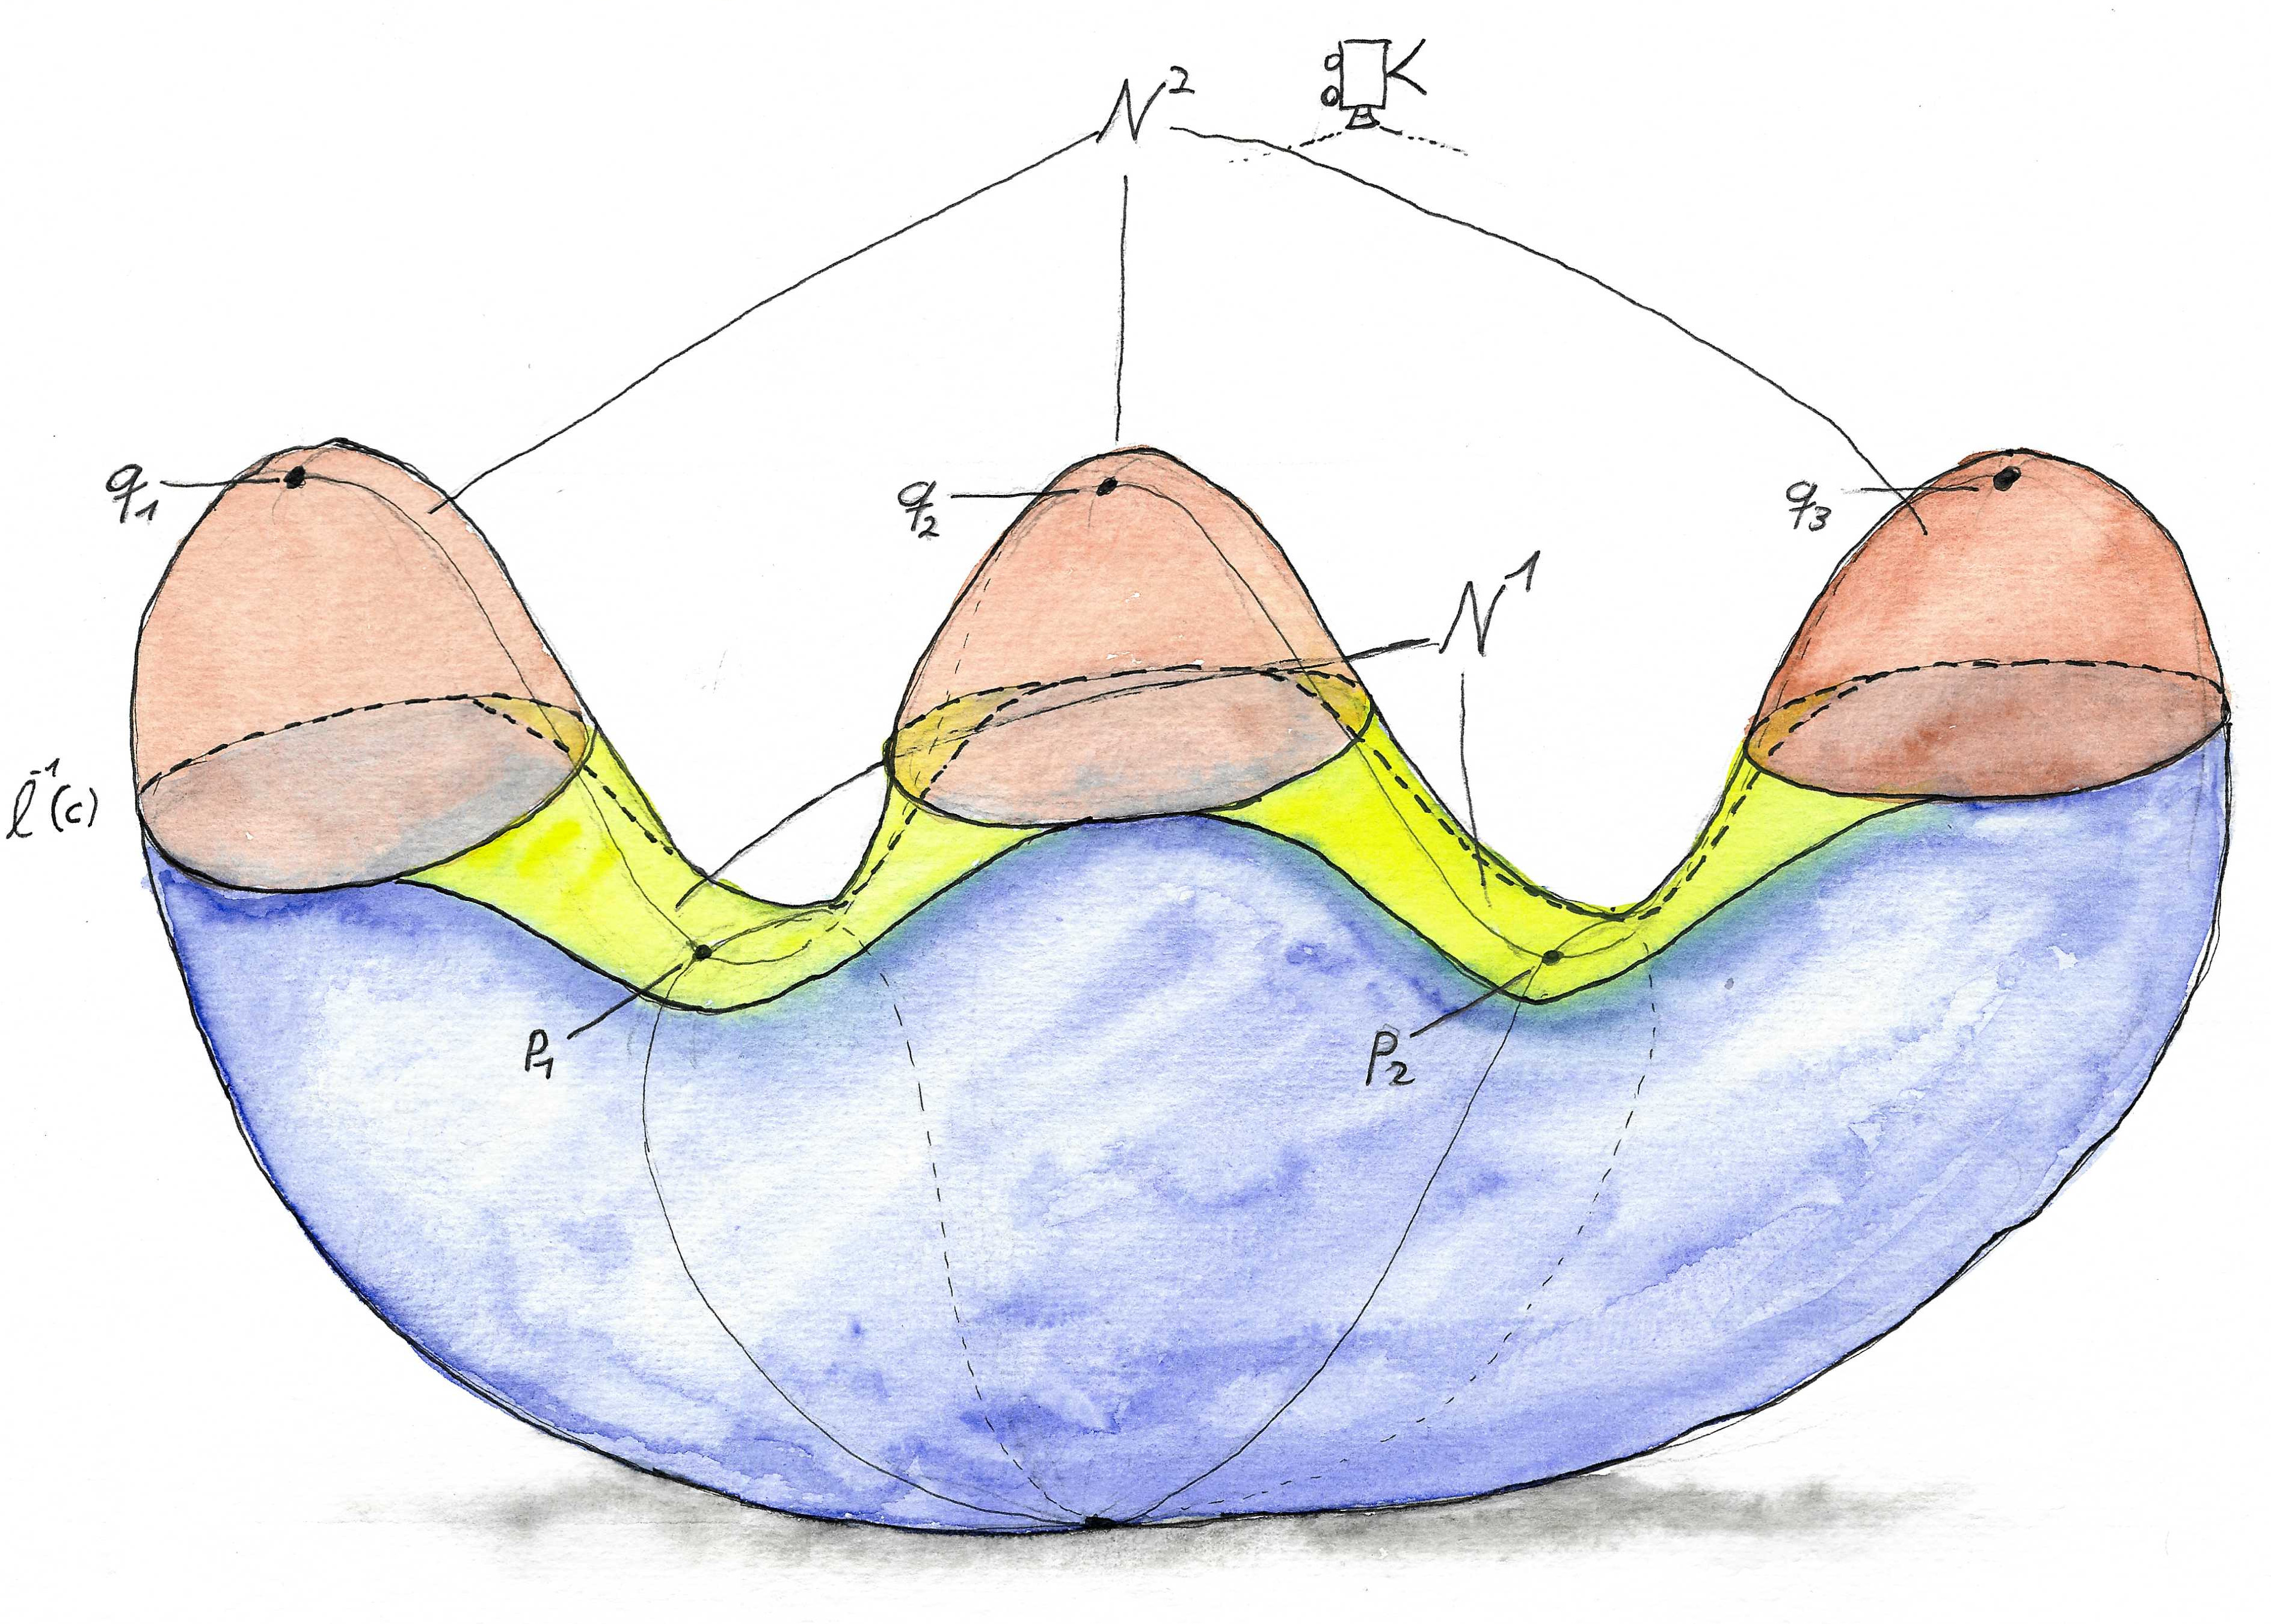
\includegraphics[width=0.49\textwidth]{text/images/sideViewDefinitionGlobalTriple.jpg}
	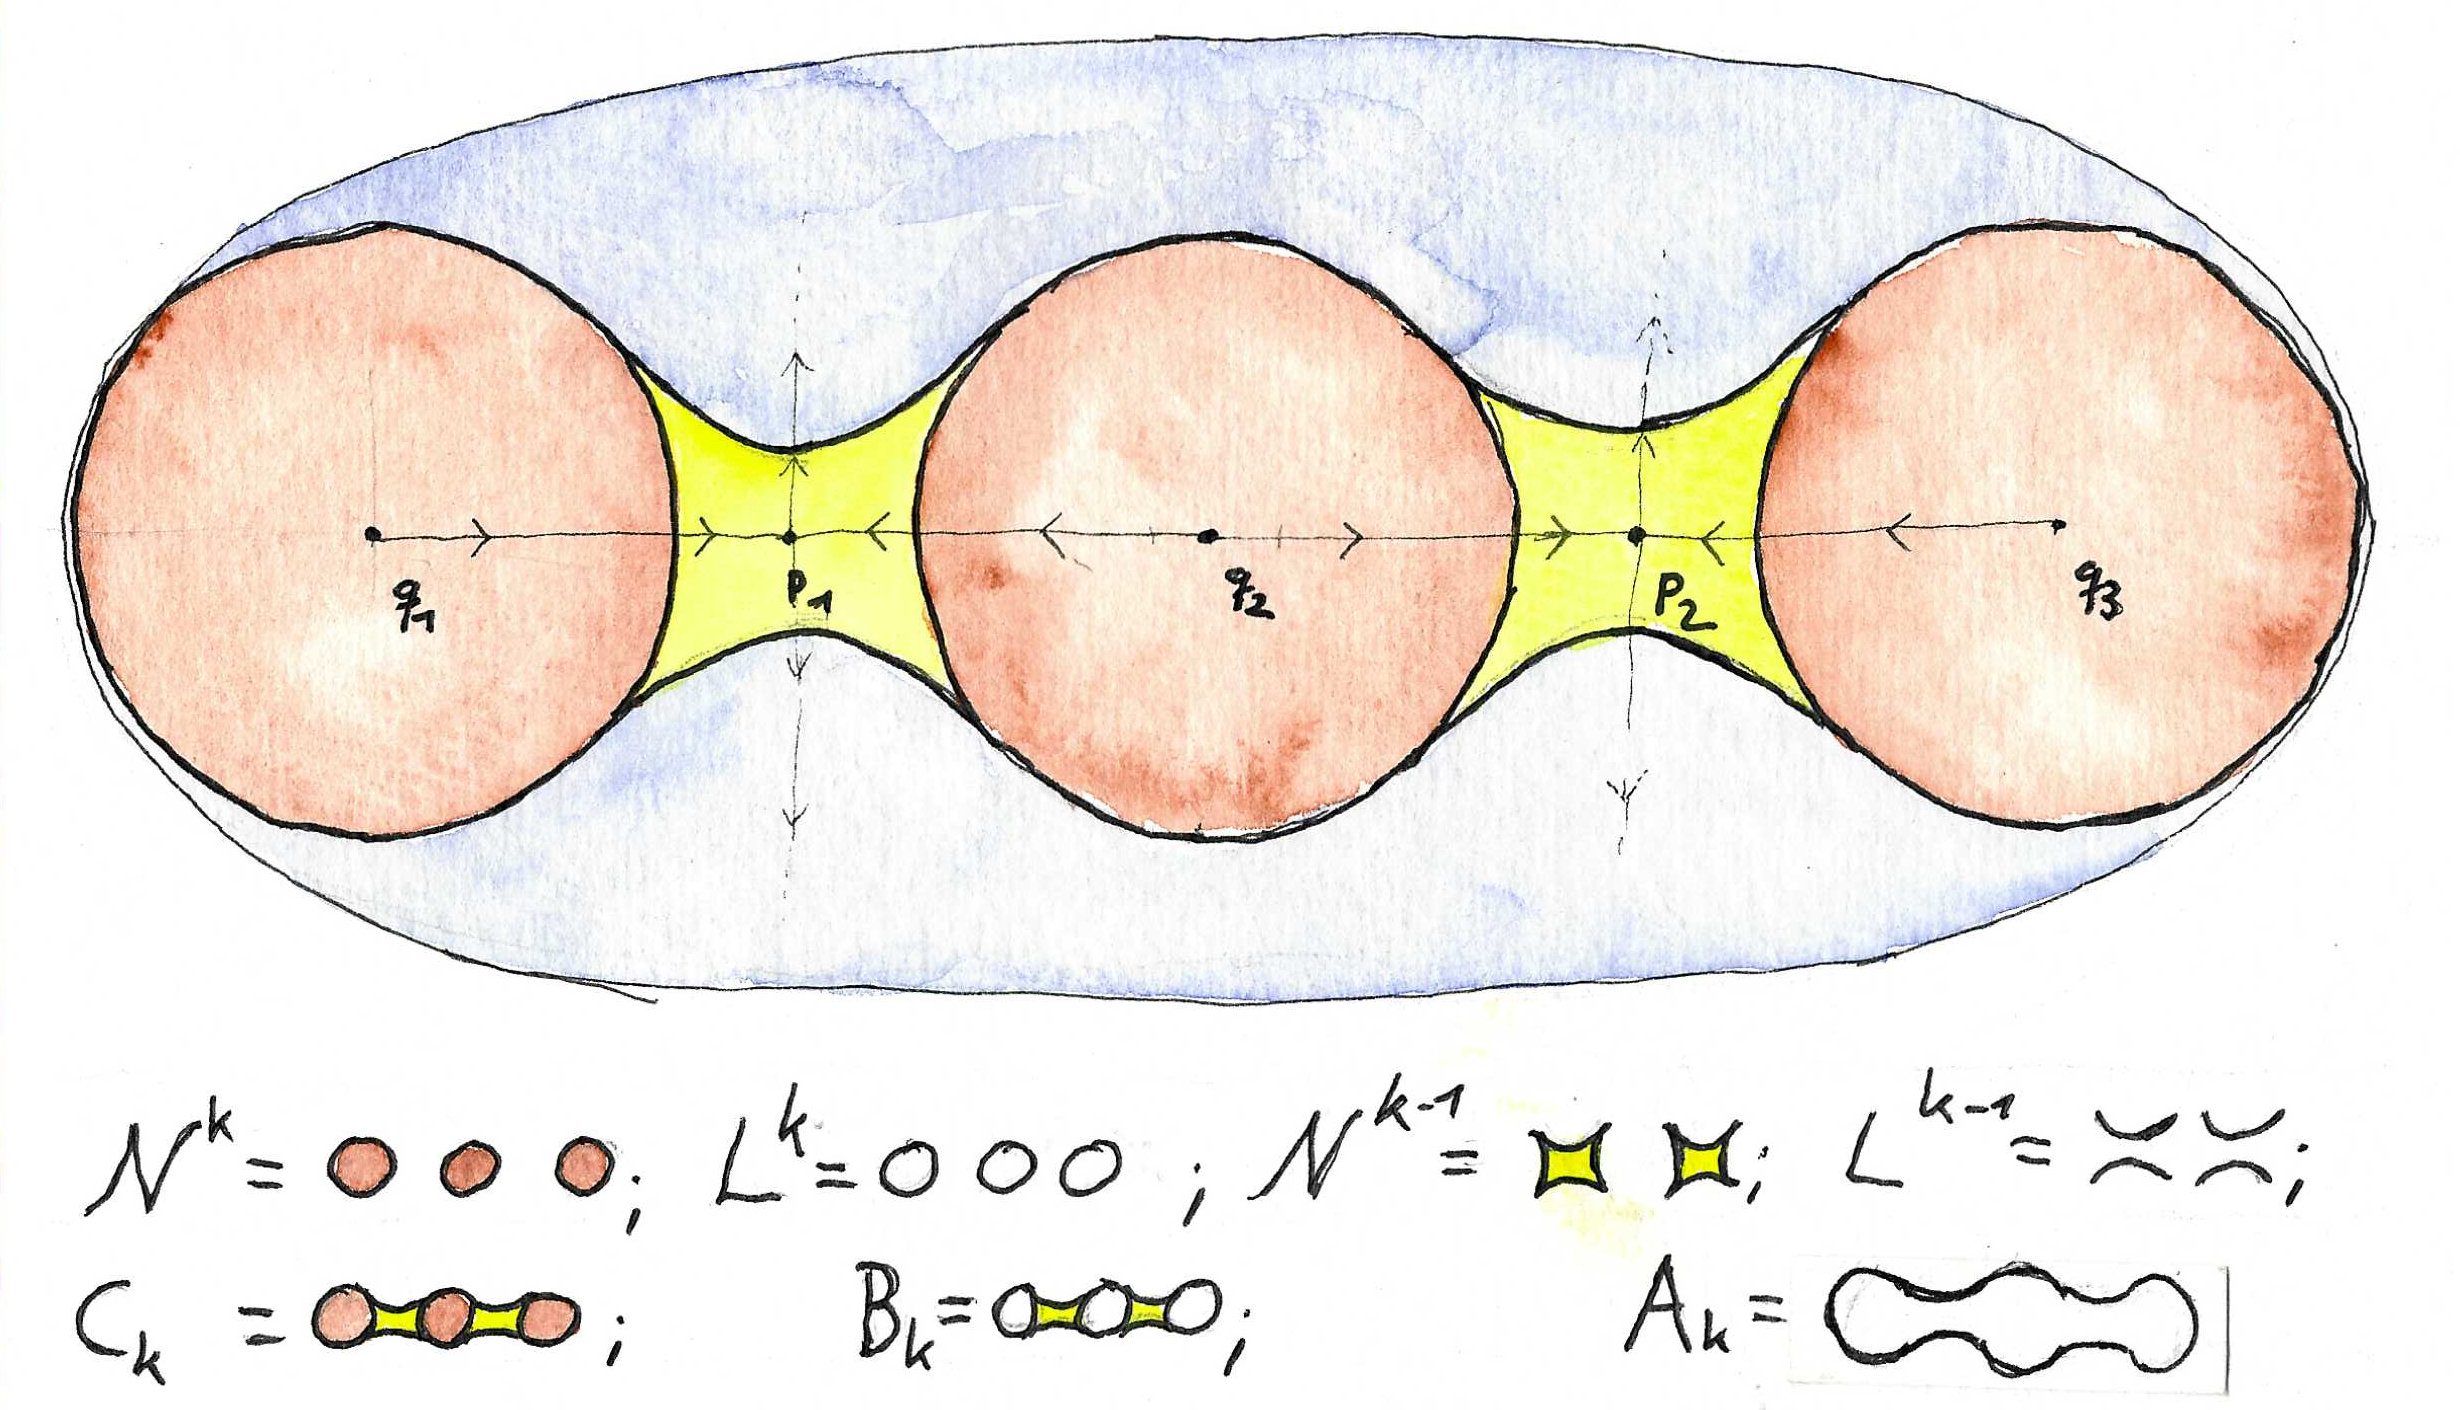
\includegraphics[width=0.49\textwidth]{text/images/TopViewDefinitionGlobalTriple.png}
	\caption{A side view on the left and top view on the right of the constructions and definitions of $N^k$ for $k=2$ from Definition \ref{def:morseFilt-globalSetup}.}\label{fig:morseFiltr-SideAndTopViewDefinitionGlobalSetup}
	\end{center}
\end{figure}

\begin{definition}[The Global Setup]\label{def:morseFilt-globalSetup}
	Let $(M,g)$ be a smooth Riemannian manifold with the Morse Smale function $f$ and orientations $\mathfrak{o}_r$ of all unstable tangend spaces $T^u_r$ for $r\in \Crit$. Let furthermore $\ell$ be an adapted Lyapunov function. Now we fix $k$, $c\in (k-1,k)$, $\epsilon \in (0,1)$ and $T>0$. With this define the sub- and superlevel sets 
	\begin{equation*}
		M_c\coloneq \ell^{-1}[c,\infty)=\{\ell \geq c\}\qquad \text{ and }\qquad M^c\coloneq \ell^{-1}(-\infty,c]=\{\ell \leq c\}\,
	\end{equation*} 
	\begin{align*}
		N^k
		&\coloneq \{x\in M_c \mid \ell(\phi_{-T}x)\le k+\epsilon\}, &
		L^k
		&\coloneq N^k\cap\ell^{-1}(c),\\
		N^{k-1} &\coloneq \{x\in M^c \mid \ell(\phi_{T}x)\ge k-1-\epsilon\}, &
		L^{k-1} &\coloneq \{x\in N^{k-1}\mid \ell(\phi_T x)=k-1-\epsilon\},
	\end{align*}and the \textbf{global triple}
	\begin{equation*}
		C_k\coloneq N^k\cup N^{k-1},\qquad
		B_k\coloneq N^{k-1}\cup L^k,\qquad
		A_k\coloneq L^{k-1}\cup\big(L^k\setminus N^{k-1}\big).
	\end{equation*}
	For the following proof we also define 
	\begin{equation*}
		S(q\to) \coloneq W(q\to)\cap \ell^{-1}(c),\qquad
		D_q \coloneq W(q\to)\cap M_c\,.
	\end{equation*}
	\todo{Hier die benötigten konventionen/oprienbtierungen einfügen}
\end{definition}


\begin{lemma}[Cantor's Intersection Theorem]\label{lem:morseFiltr-cantorsIntersectionTheorem}
	Let $C_k$ be a family of compact spaces non-empty such that $C_k\supseteq C_{k+1}$ for all $k\in I$, where $I$ is an ordered set containing smallest element $1\in I$. Then the intersection 
	$\bigcap_{k\in I} C_k \neq \emptyset$ is non-empty.
\end{lemma}
\begin{proof}
	Assume the opposite, that $\bigcup_{k\in I} C_k=\emptyset$.
	 As we defined compact spaces to be hausdorff, we can conclude that all $C_k$ are closed and thereby $U_k\coloneq C_1\setminus C_k$ is open in $C_1$. Now by our assumption, the $U_k$ cover $C_1$ (for every $x\in C_1$ there exists a $k\in I$ such that $x\notin C_k$ and hence $x\in U_k$). As $C_1$ is compact, there is a finite ascending subfamiliy that already covers $C_1=U_{k_1}\cup \cdots \cup U_{k_m}$, where ascending means that $U_{k_i}\subseteq U_{k_{i+1}}$. Hence, $C_1=U_{k_m}=C_1\setminus C_{k_m}$ (notice, that we used existence of maximum elements in finite ordered sets), and as $C_{k_m} \subseteq C_1$ this implies that $C_{k_m}=\emptyset$ which contradicts our assumtion. Hence, by contraposition, we arrived at the statement. 
\end{proof}
\begin{lemma}[Splitting into Pieces]\label{lem:morseFilt-piecesOfGlobalSetup}
	Choose pairwise disjoint open subsets $U_q\supseteq D_q$ ($q\in \Crit_k(f)$)and $U_p\subseteq W(\to p)\cap M^c$ ($p\in \Crit_{k-1}(f)$). For $T$ large enough 
	$N^k\subseteq \bigsqcup_q U_q$ and $N^{k-1}\subseteq \bigsqcup_p U_p$. In this setting
	\begin{equation*}
		N_q\coloneq N^k 	\cap U_q, \quad L_q \coloneq L^k    \cap U_q,\quad 
		N_p\coloneq N^{k-1} \cap U_p, \quad L_p \coloneq L^{k-1}\cap U_p
	\end{equation*} are compact, $N^k=\bigsqcup_qN_q$, $L^k=\bigsqcup_q L_q$, $N^{k-1}=\bigsqcup_p N_p$ and $L^{k-1}=\bigsqcup_p L_p$.
\end{lemma}
\begin{proof}
	Notice, that the limit $\bigcap_{T\in \R_{>0}} N^k=\bigsqcup_q D_q$: If $x\in D_q$ then $\phi_{-T}\in D_q$ for all $T$ and hence $x\in \bigcap_{T\in \R_{>0}} N^k$. Is on the other hand $x\notin D_q$ for any $q\in \Crit_k$ hence $x\notin W(q\to)\cap M^c$, then $x\in W(r\to)$ for some $r$ with $\ind(r)\neq k$, and as $\ell(r)\geq \ell(x)>{k-1}$, we know that $\ind(r)>k$. Thereby, $\phi_{-T}(x)$ approaches $r$ implying that $\ell(\phi_{-T}(x))$ approaches $\ind(r)\geq{k+1}$ and hence, for $T$ big enough $\ell(\phi_{-T}(x))\geq k+\epsilon$, concluding that indeed $\bigcap_{T\in \R_{>0}} N^k=\bigsqcup_q D_q$.


	Now the $D_q$ themself are compact, as by the $\lambda$-Lemma, the boundary of $D_q$ is given by unstably manifolds of critical points of lower degree. Hence, their $\ell$-value is below $c$ and we could rewrite our intersection $W(q\to)\cap M^c$ to become $\overline{W(q\to)\cap M^c}$ which in turn is the intersection of two compact spaces and thereby compact again.


	Finally, For every $T$, the $N^k_T$ are compact (as they are given by a closed condition on a compact manifold). Hence, if we assume $T$ to be increasing to infinity, we have a decending family of compact spaces that approaces $\bigsqcup_q D_q$. Assume that $N^k_T$ would never be contained in our neighbourhoof $\bigcup_q U_q$. Then for all $T$, $N^k_T\setminus U$ would be non-empt, compact, and again a decending family, meaning that the intersection $\bigcap_T (N^k_T\setminus U)\neq \emptyset$ by Cantor's intersection Theorem \ref{lem:morseFiltr-cantorsIntersectionTheorem}. This however contradicts that the $N^k_T$ approach $\bigsqcup_q D_q$.

	The same argument (where instead of the $-T$-limit we take toe $T$-limit) shows that $N^k$ is contained in an open neighbourhood $\bigsqcup_p U_p$ for $T$ big enough. The rest of the lemma follows imidiatly from the fact that the intersections seperate disjoint pieces of a compact space, which are compact themself.
\end{proof}
From now on, the notations from Definition \ref{def:morseFilt-globalSetup} and Lemma \ref{lem:morseFilt-piecesOfGlobalSetup} is used.

\begin{lemma}[The Global Triple]\label{lem:morseFilt-globalTriple}
	For $\epsilon$ small and $T$ large: 
	\begin{enumerate}[(i)]
		\item $A_k$ is closed, and $(C_k,A_k)$ is an index pair of $S_k$.
		\item $B_k=A_k\cup \big(C_k \cap \ell^{-1}(-\infty,c]\big)$, hence $(C_k,B_k,A_k)$ is a sublevel triple for $S_k$.
		\item the inclusions induce homeomorphisms:
			\begin{equation*}
				\bigvee_q N_q/L_q = N^k/L^k \xrightarrow{\ \cong \ } C_k/B_k\,,\qquad
				\bigvee_p N_p/L_p = N^{k-1}/L^{k-1} \xrightarrow{\ \cong \ }B_k/A/k\,. 
			\end{equation*}
		\item $(N_q,L_q)$ is an index pair of $\{ q\}$ and $(N_p,L_p)$ of $\{p\}$.
		\item For every neighbourhoof $U$ of $W(\to p)\cap \ell^{-1}(c)$ that is open in $\ell^{-1}(c)$ there is a $T$ such that $N_p\cap \ell^{-1}(c)\subseteq U$.
	\end{enumerate}
\end{lemma}
\begin{proof}
	$A_k$ is colsed, as $L^{k-1}$ is closed and the closure 
	\begin{equation*}
		\overline{L^k\setminus N^{k-1}}=L^k\setminus \inti( \underbrace{N^{k-1} \cap L^k}_{N^{k-1}\cap \ell^{-1}(c)})=L^k\setminus N^{k-1}\cap \partial N^{k-1}\cap L^k
	\end{equation*} is only gaining the points $\partial N^{k-1}\cap L^k=\{\ell \circ \phi_T=k-1-\epsilon\}\subseteq L$ which are already in $L^{k-1}$. 
	
	(i) We need to check the three properties:
	\begin{enumerate}
		\item  It is clear that for all $T$ and $\epsilon$ $S_k\subseteq \inti(A_k \setminus C_k)$, as $N^k \cup N^{k-1}$ give an open neighbourhood of the closed $S_k$, and $A_k\subseteq \partial N^k\cup N^{k-1}$. The latter is true, as any element  $x\in A_k$ is either in $L^{k-1}\subseteq \partial N^{k-1}\setminus \overline{N^k}$, or in $L^{k-1}\setminus N^{k-1}$. But $L^{k-1}\setminus N^{k-1}\subseteq \partial N^k \setminus  \overline{N^{k-1}}$. Since $S_k$ is invariant, we have that for all $T,\epsilon$ $S_k\subseteq I(\overline{C_k\setminus A_k})$. Now for any $T>0$, and any $\epsilon \in (0,1)$ $x\in C_k\in \ell^{-1}(k-1-\epsilon,k+\epsilon)$. The flow invariant subset $I(\overline{C_k\setminus A_k})$ is contained in the flow invariant subset $I(\overline{\ell^{-1}(k-1-\epsilon,k+\epsilon)})\subseteq I(\ell^{-1}(k-2,k-1))$.
	For any $x\in \ell^{-1}(k-2,k-1)$, the limit $\lim_{s\to \pm \infty} \phi_s(x)$ either stays in the cylinder $\ell^{-1}(k-2,k-1)$ and thereby $x\in W(q\to p)\subseteq S_k$ for some $q\in \Crit_k$, $p\in \Crit_{k-1}$, or it leaves the cylinder. Hence, $I(\overline{C_k\setminus A_k}) \subseteq S_k$ and with the containmend above we can conclude, that $S_k=I(\overline{C_k\setminus A_k})$.
		\item  The positive invariance of $A_k$ in $C_k$ is a direct consequence of $\ell$ decending along the flow $\phi_s$.
		\item The exit set property is also a direct consequence of $\ell$ decending along the flow $\phi_s$.
	\end{enumerate}

	(ii) This is just a reformulation:
	\begin{equation*}
		A_k\cup \underbrace{(C_k\cap \ell^{-1}[-\infty,c))}_{=C_k\cap M^c=N^{k-1}\cup L^k}=\underbrace{L^{k-1}}_{\subseteq N^{k-1}}\cup (L^k\setminus N^{k-1})\cup N^{k-1} \cup L^k =L^k\cup N^{k-1}
	\end{equation*}
	(iii) Obviously $N^k/L^k \to C_k / B_k$ is a homeomorphism, as the inclusion induces a continuous bijection between two compact and Hausdorff spaces. The same argument works for $N^{k-1}/L^{k-1}\to B^k/ A_k$ once we realice, that if $x\in B^k$ but $x\notin N^{k-1}$ then $x\in L^k\setminus N^{k-1}\subseteq A_k$. 

	(iv) By (ii) and Lemma \ref{morseFiltr-sublevelTripoleGivePairs} (together with (iii) )we know that $(C_k,B_k)$ is an index pair for $\Crit_k$ and $C_k=\sqcup_q N_q$, where the $N_q$ are closed and open in $C_k$. Hence, $(N_q,B_k\cap N_q)$ is an index pair of $\{q\}$, as all properties translate to the smapper space that only contains $\{q\}$ as an invariant subset and finally 
		\begin{equation*}
			B_k\cap N_q=(N^{k-1}\cup L^k)\cap N_q=\underbrace{(N^{k-1}\cap N_q)}_{\subseteq (N^k\cap N^{k-1})\cap N_q \subseteq L^k \cap N_q}\cup (L^k\cap N_q)=L_q
		\end{equation*}
		Hence, $(N_q,B_k\cap N_q)=(N_q,L_q)$ is an index pair of $\{q\}$ and similar we can show that $(N_p,L_q)$ is an index pair of $\{p\}$.

	(v) Similar to the proof of Lemma \ref{lem:morseFilt-piecesOfGlobalSetup}: Assume that $T$ is increasing to infinity. Notice how the intersection $\bigcap_T (N_p \cal \ell^{-1}(c))=(W(\to p)\cup \{p\})\cap \ell^{-1}(c)$. Let $U$ be a neighbourhood of $W(\to p)\cap \ell^{-1}(c)$ and assume that for all $T$, the intersection $\big(N_p\cap \ell^{-1}(c)\big)\cap U^c\neq \emptyset$ where $U^c$ denotes the complement of $U$. Then by Canotrs intersection Theorem \ref{lem:morseFiltr-cantorsIntersectionTheorem}, the intersection $\cap_T \big(N_p\cap \ell^{-1}(c)\big)\cap U^c \neq \emptyset$ which contradicts $\cap_T (N_p \cal \ell^{-1}(c))=(W(\to p)\cup \{p\})\cap \ell^{-1}(c)$ and thereby the final statement is shown.
\end{proof}
\begin{definition}[Lokal Triple]\label{def:morseFiltr-localTriplaABC}
	We define the local triple 
	\begin{equation*}
		C^{qp}\coloneq N_q\cup N_p\,\qquad B^{qp}\coloneq N_p\cup L_q\,,\qquad A^{qp}\coloneq L_p \cup (L_q\setminus N_p)\,.
	\end{equation*}
\end{definition}
\begin{lemma}[Restricting to Summands]\label{lem:morseFiltr-restrictingToSummand}
	Let $i_q:N_q/L_q \to \bigvee_{q'\in \Crit_k}N_{q'}/L_{q'}$ be the inclusion of a summand and $c_p:\bigvee_{p'\in \Crit_{k-1}}N_{p'}/L_{p'}\to N_p/L_p$ the collaps of everything but one summand. Under the identifications of Lemma \ref{lem:morseFilt-globalTriple}(iii) and $C^{qp}/B^{qp}=N_q/L_q$, $B^{qp}/A^{qp}=N_p/L_p$,
	\begin{equation*}
		i_q^* \circ \delta_{triple}^{(C_k,B_k,A_k)}\circ c_p^*\;=\; \delta_{triple}^{(C^{qp},B^{qp},A^{qp})}\,.
	\end{equation*}
	In particular,
		$\pcomp{(\Delta^{k-1})^{q}_p} = \pcomp{\big(b\circ \delta_{triple}^{(C^{qp},B^{qp},A^{qp})} \big)}$, or globally:
		\begin{equation*}
			 \Delta^{k-1}=
		\end{equation*}
\end{lemma}
\begin{figure}
	\begin{center}
		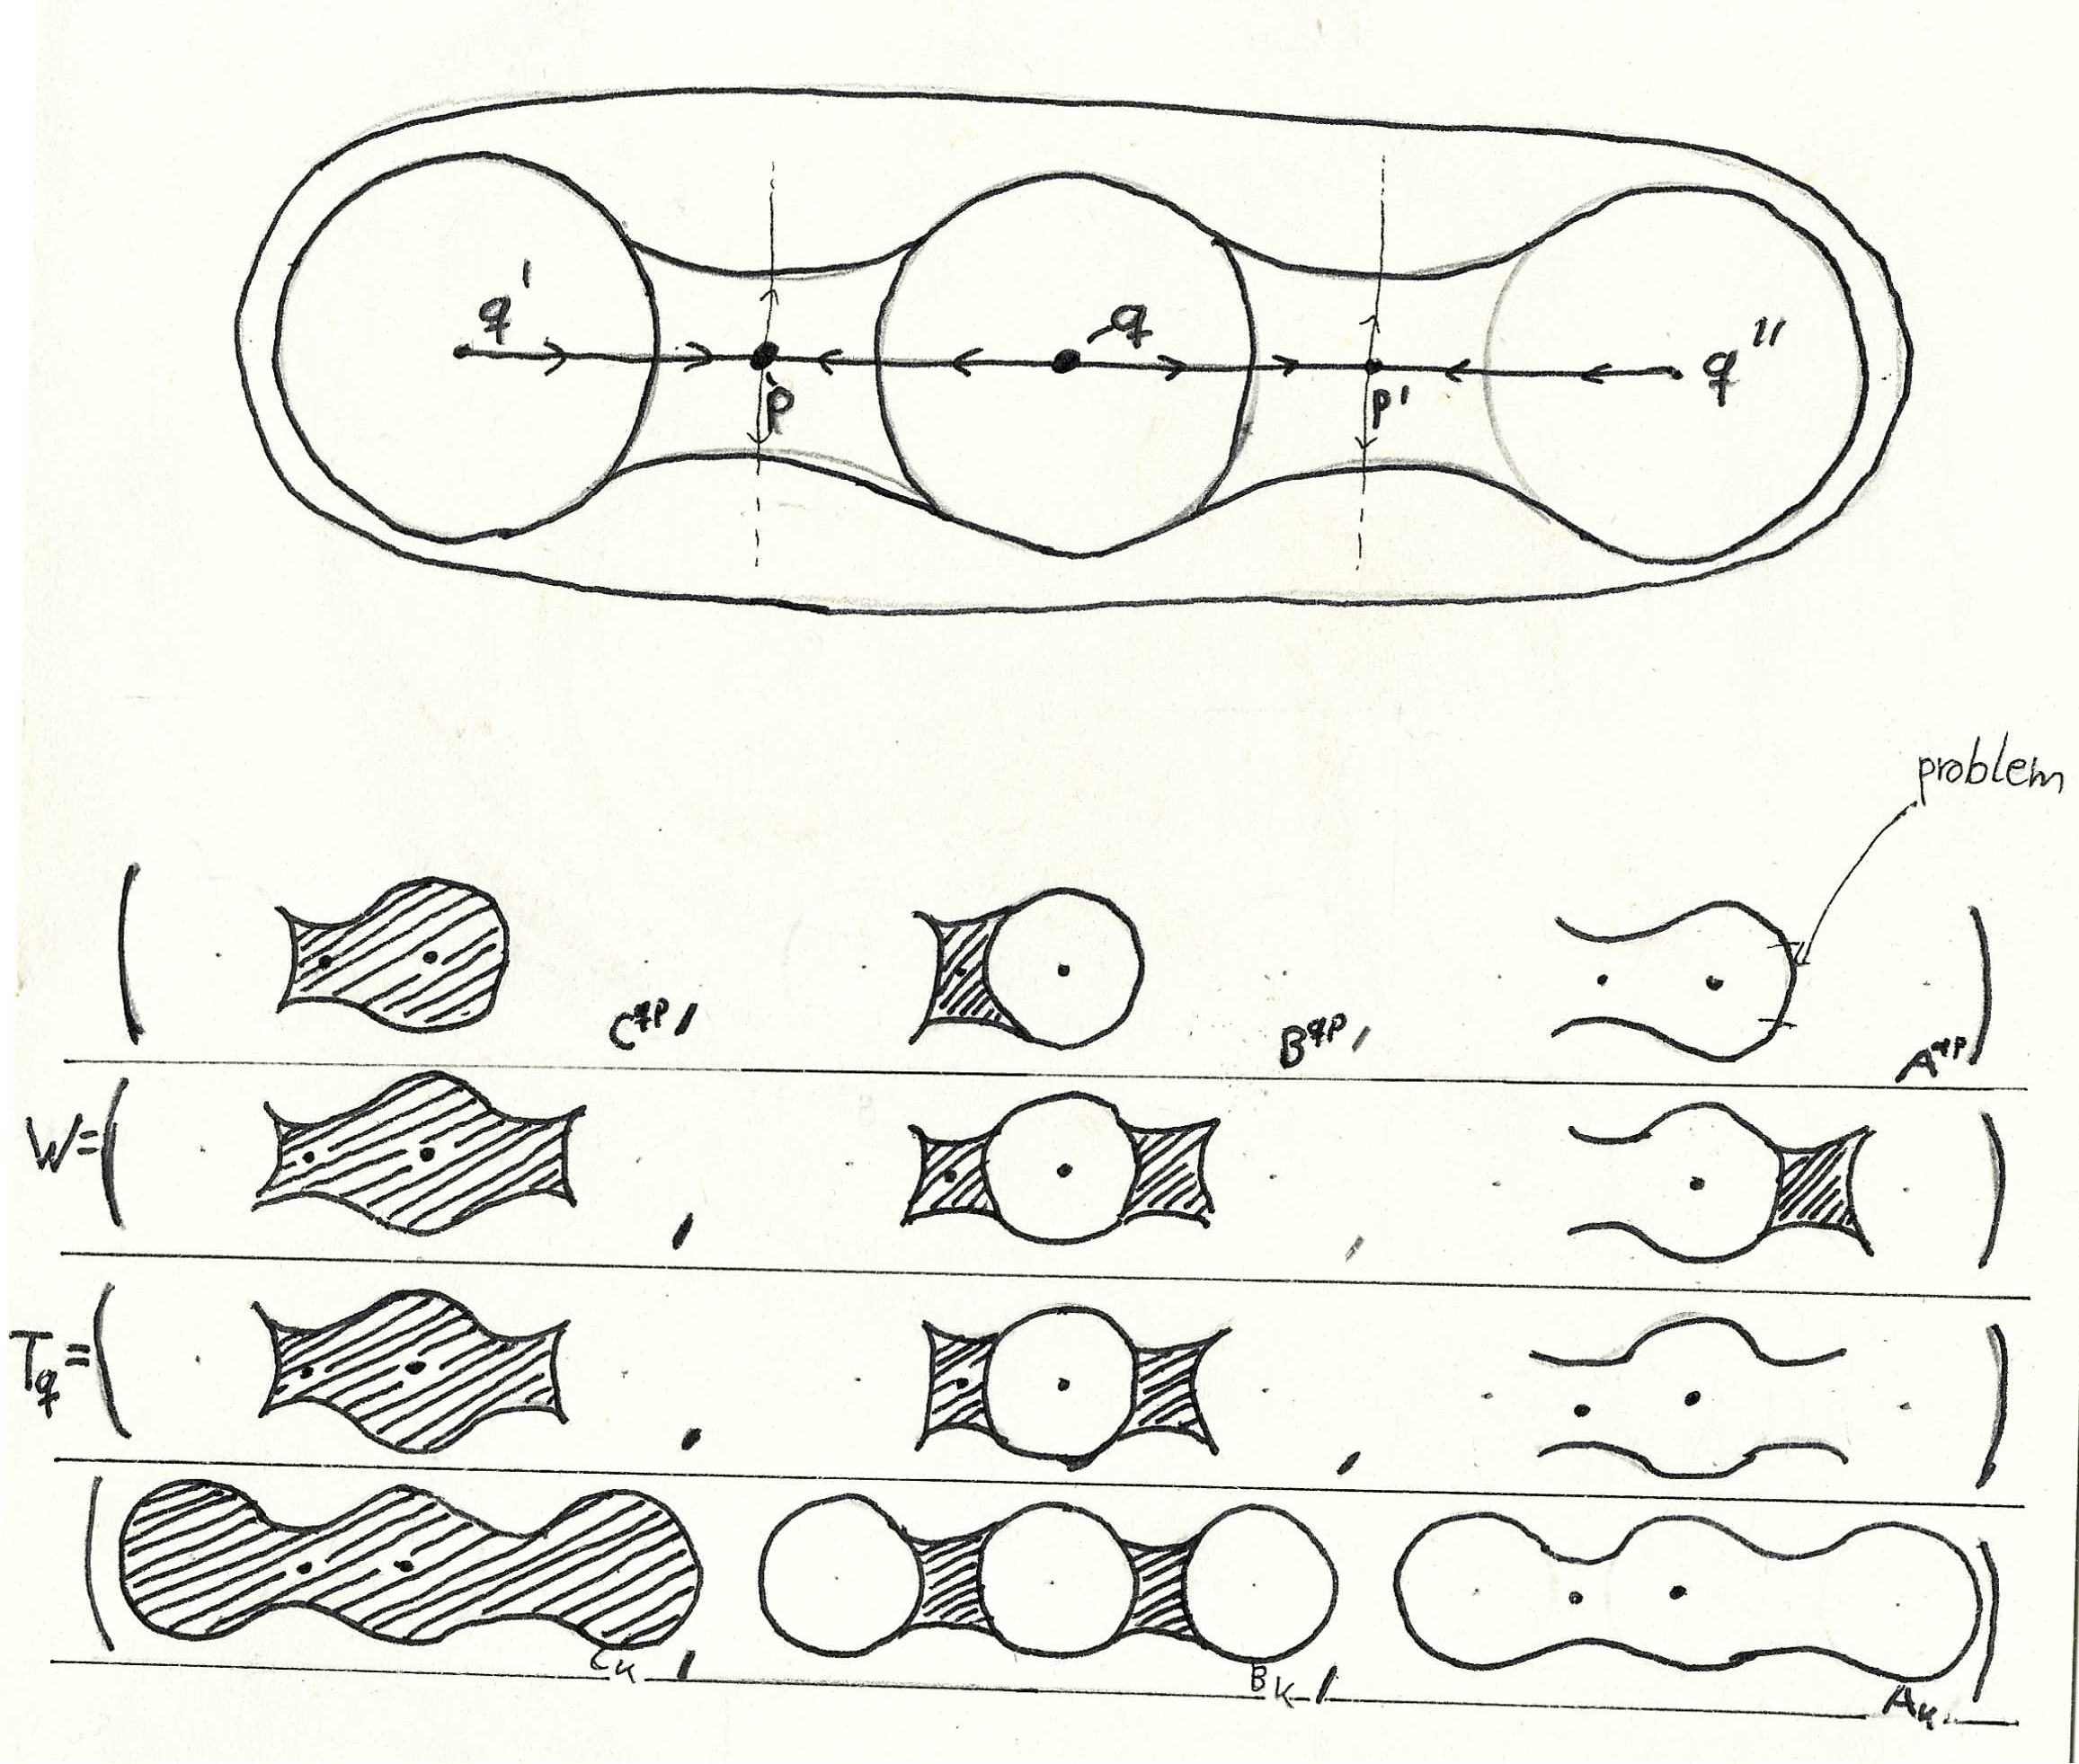
\includegraphics[width=0.7\textwidth]{text/images/restrictingToASummand.png}
	\caption{The triples of Proof of Lemma \ref{lem:morseFiltr-restrictingToSummand}. The image continuous the exampe esteblished in Figure \ref{fig:morseFiltr-SideAndTopViewDefinitionGlobalSetup}}\label{fig:MorseFiltr-theTriplesInRestrictionOfSummondsProof}
	\end{center}
\end{figure}
\begin{proof}
	This does not follow immidiatly, as the inclusion $(\qp{C},\qp{B},\qp{A})\hookrightarrow (C_k,B_k,A_k)$ is not a map of triples. This can be seen as there are elements in $L_q\setminus N_q$ that fo not live in $A_k$ but in $B_k$ (Compare Figure \ref{fig:MorseFiltr-theTriplesInRestrictionOfSummondsProof}, where the proplematic area is marked). So we go through intermediate triples
		\begin{align*}
			T_q &\coloneq \big(N_q \cup N^{k-1},\; L_q \cup N^{k-1},\; L^{k-1}\cup (L_q \setminus N^{k-1})\big)\,,\\
			W   &\coloneq \big(N_q\cup N^{k-1},\; L_q\cup N^{k-1},\;
						       L_p\cup \bigcup_{p'\in \Crit_{k-1}\setminus\{p\}}N_{p'}\cup (L_q\setminus N^{k-1})\big)\,,
		\end{align*}
	and get the maps of triples (all induced by the inclusions)
	\begin{equation*}
		(C_k,B_k,A_k)\xleftarrow{\ \iota_1\ }T_q \xrightarrow{\ \iota_2 \ } W \xleftarrow{ \ \iota_3 \ }(\qp{C},\qp{B},\qp{A})
	\end{equation*}
	In the quotient of the first two summands of the triples, the maps induce 
	$i_q$, $\id_{N_q/ L_q}$ and $ \id_{N_q/ L_q}$. In the quotients of the second and third summands of the triples the three maps induce the maps
	$\id_{N^{k-1}/L^{k-1}}$, $c_p$ and $\id_{N_p/L_p}$. 
	Here we always identified the quotiends of the second by the third summands of the triples with $N^{k-1}/L^{k-1}$ 
	respectifely with $N_p/L_p$ via the inclusion as in Lemma \ref{lem:morseFilt-globalTriple} (iii). Now naturality of the triple connecting homomorphism gives
	\begin{equation*}
		\delta_{triple}^{T_q}=i_q^* \circ \delta^{(C_k,B_k,A_k)}_{triple},\qquad
		\delta_{triple}^{T_q} \circ c_p^*=\delta_{triple}^{W}\,,\qquad
		\delta_{triple}^{(C^{qp},B^{qp},A^{qp})}=\delta_{triple}^W\,. 
	\end{equation*}
	Now by definition (compare Corollary \ref{cor:morseFilt-summandsAndFactorsOfMorphisms}), and the calculations of Remark \ref{rem:MorseFiltr-ProductStruktureOfKIPk} we calculate
	\begin{align*}
		(\Delta^{k-1})^{q}_p
		&=\pcomp{pr_q}circ \Delta^{k-1}\circ \pcomp{i_p}\\
		&= \pcomp{i_q^*}\circ \pcomp{\left(b\circ \delta^{(C_k,B_k,A_k)}_{triple}\right)} \circ \pcomp{c^*_p}\\
		&=\pcomp{b}\circ \pcomp{i_q^*}\circ \pcomp{ \delta^{(C_k,B_k,A_k)}_{triple}} \circ \pcomp{c^*_p}\\
		&=\pcomp{b}\circ \pcomp{\delta_{triple}^{T_q}} \circ \pcomp{c^*_p}\\
		&=\pcomp{b}\circ \pcomp{\delta_{triple}^{W}}\\
		&=\pcomp{\left(b\circ \delta_{triple}^{(C^{qp},B^{qp},A^{qp})}\right)}
	\end{align*}
	The global statement is just the calculation (again with Corollary \ref{cor:morseFilt-summandsAndFactorsOfMorphisms} and  Remark \ref{rem:MorseFiltr-ProductStruktureOfKIPk}): 
	\begin{align*}
			 \Delta^{k-1}
			 &=\sum_p\left(\sum_q \left(\pcomp{i_q} \circ \pcomp{(\Delta^{k-1})^{q}_p}\right)\pcomp{pr_p}\right)\\
			 &=\sum_p\left(\sum_q \left(\pcomp{c^*_q} \circ \pcomp{(\Delta^{k-1})^{q}_p}\right)\pcomp{i^*_p}\right)\\
			 &=\sum_p \sum_q \pcomp{ \left(c^*_q\circ \left(b\circ \delta_{triple}^{(C^{qp},B^{qp},A^{qp})}\right) \circ i^*_p\right)}
	\end{align*}
\end{proof}

 \begin{comment}
\begin{definition}[Definitions and Setup]\label{def:morseFilt-setupCommutingDiff}
	We work in a compact, Riemanian, smooth manifold $(M,g)$ of dimension $m$ together with a Morse-Smale function 
	\begin{align}
		f: M\to \R
	\end{align} and orientations $\mathfrak{o}$ of all unstable tangent spaces. We denote the flow corresponding to the negative gradient by $\phi_t(x)$.
	We assume that $q$ is a critical point of index $k$ and $p$ is a critical point of index $k-1$. We define $f(q)=b$ and $f(p)=a$ and assume that there is no critical point in $f^{-1}(a,b)\subseteq M$. We define the sublevle and superlevel sets 
	\begin{align}
		M^t \coloneq \{ x\in M | f(x)\leq t \} \quad \text{and}\quad M_t:=\{ x\in M | f(x)\geq t \} \, ,
	\end{align} and the constants 
	\begin{align}
		c \in (a,b) \quad , \quad \epsilon >0 \text{ small } \quad,\quad T>0 \text{ big .}
	\end{align} With this we define the sets: 
	\begin{align}
		N_q  & \coloneq    \{ x\in M_c |f(\phi_{-T}(x))  \leq b+ \epsilon  \}   \, ,  \\
		L_q  & \coloneq    \{ x\in N_q |f(x)             =    c            \}    \, , \\
		N_p  & \coloneq    \{ x\in M^c |f(\phi_T(x))     \geq a-\epsilon   \}    \, , \\
		L_p  & \coloneq    \{ x\in N_p |f( \phi_T(x))    =    a-\epsilon   \} \, ,
	\end{align} and finally: 
	\begin{align}
		C  & \coloneq  N_p \cup N_q  \, ,                     	\\
		B  & \coloneq  N_p \cup L_q   \, ,                   	\\
		A 	 & \coloneq  L_p \cup \inti{(L_q\setminus N_p)} 			\\
		S(q\to)& \coloneq W(q\to)\cap f^{-1}(c)\				\\
		D_q & \coloneq W(q\to)\cap M_c\,.							
	\end{align}
	
	
	Furthermore, we assume $W(q\to)$ to be oriented with respect to the orientation of $T^u_qM$ as in Proposition \ref{prop:morse-OrientedUnstableSpaces}. Let $Q^p\coloneq \restr{TM}{W(\to p)}\Big/ TW(\to p)$ be oriented with respect to $T^u_pM$ as in Proposition \ref{prop:morse-orientTheQuotient}.
	For an oriented real vector space $V$ of dimension $n$, let $\beta_V\in K^{-n}(\overline{V})$ denote its K-theoretic orientation from Corollary \ref{cor:orient-vectorspaceOrientationInducesKtheoreticOrientation}. For an index pair $(N,L)$ of $\{p\}$ let $\alpha^{(N,L)}_p\in K^{-\ind_p}(N,L)$ denote the canonical generator from Remark \ref{rem:morseFiltr-morphismToCanonicalIntegers}, i.e.\ the pullback of $\kappa_p^*(\beta_{T^u_pM})$ along the homotopy equivalence of Theorem \ref{thm:morseFiltr-homotopyEquivalenceOfIndexPairs} from $(N,L)$ to the standart index pair and $\kappa_v= \kappa_q\coloneq R_0\circ \restr{\diff \phi^{-1}}{0}\circ s\circ \mathrm{pr}_u \circ \phi$. \todo{später}

	Let $(\alpha_p)_{\#}$ be a generator of $K^{\lambda_p}_{\#}(\mathcal{IP}_p)$ meaning that $(\alpha_p)_{\#}$ is a family of generators for all groups in $K^{\lambda_p}_{\#}(\mathcal{IP}_p)$ that transform into each other under the canonical group isomorphisms.
 Notice that $(\alpha_p)_{\#}$ is induced by any of its elements.
	\begin{center}
	
	
	\tikzset{every picture/.style={line width=0.75pt}} %set default line width to 0.75pt        
	\resizebox{\linewidth}{!}{%
		
		
		
		\tikzset{every picture/.style={line width=0.75pt}} %set default line width to 0.75pt      
		
		\tikzset{every picture/.style={line width=0.75pt}} %set default line width to 0.75pt        
		
		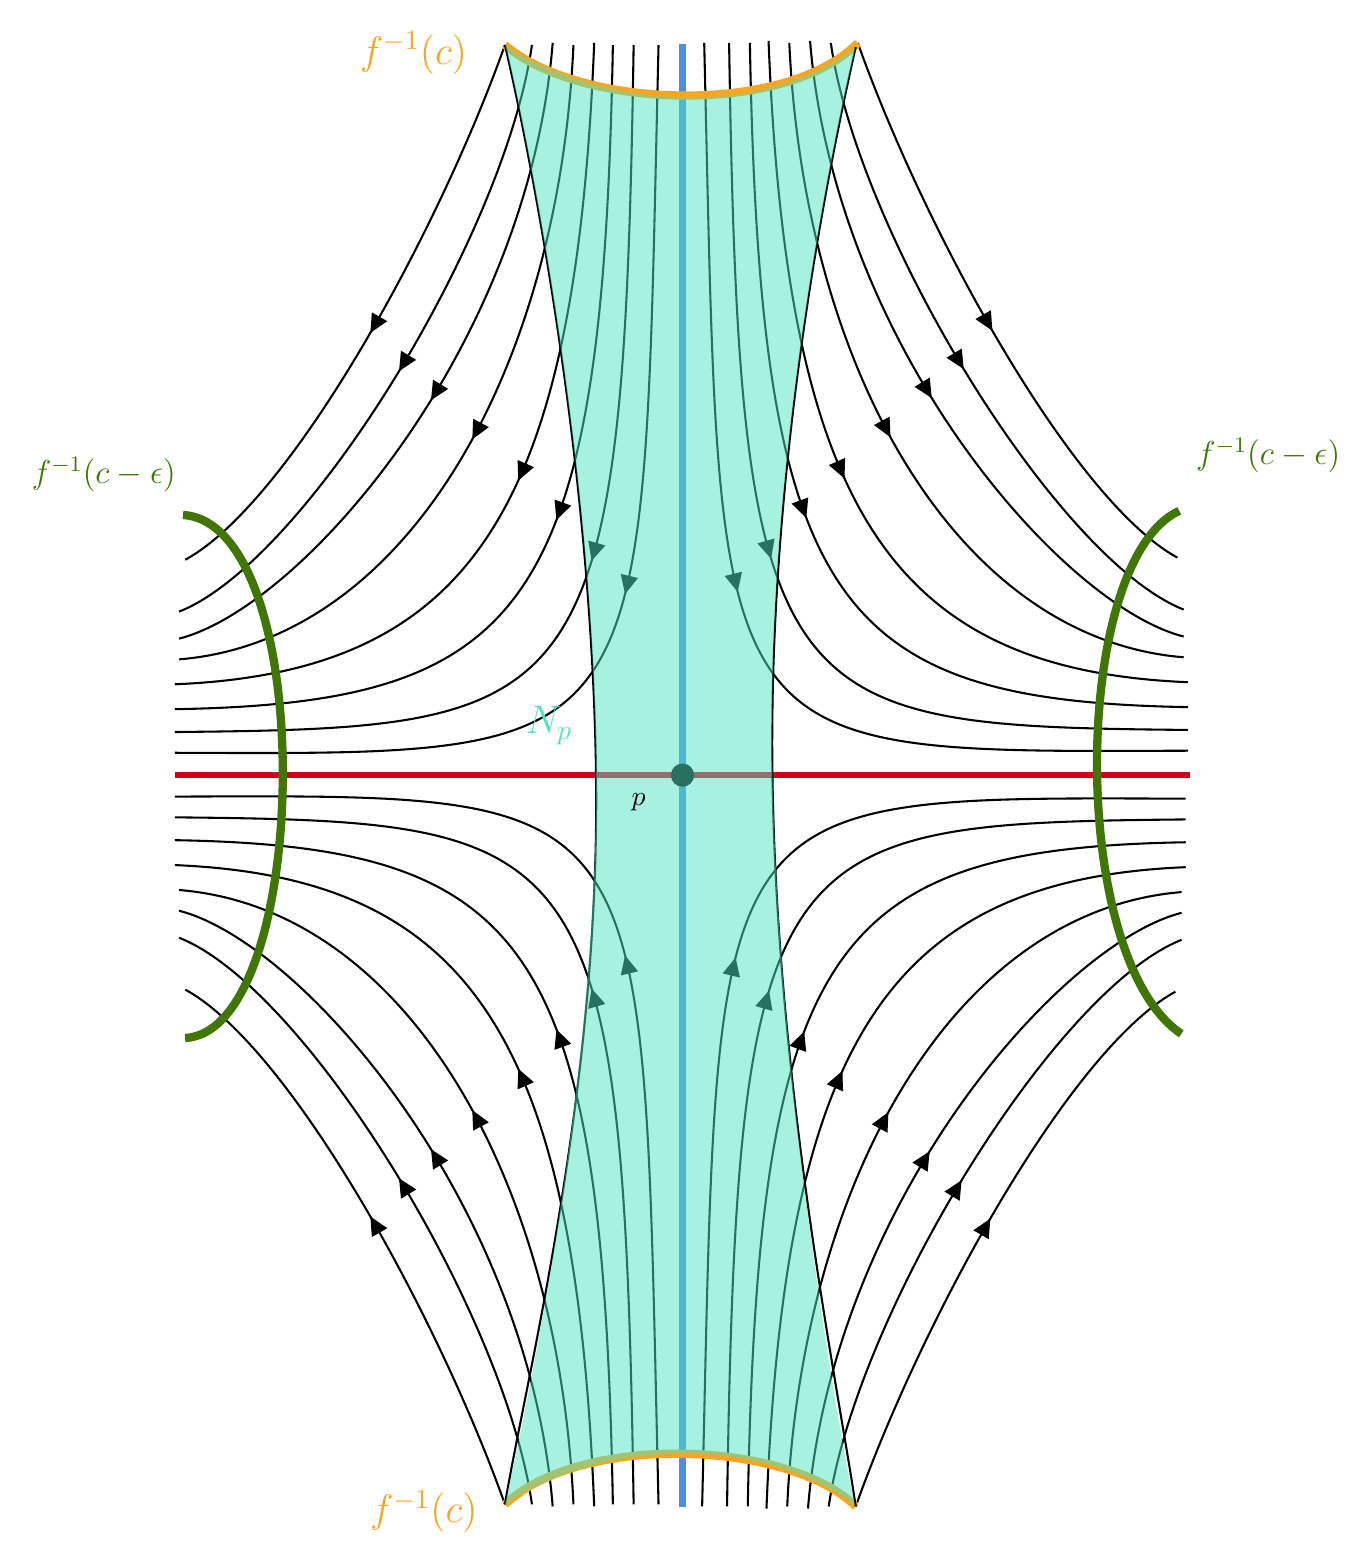
\begin{tikzpicture}[x=0.75pt,y=0.75pt,yscale=-1,xscale=1]
			%uncomment if require: \path (0,843); %set diagram left start at 0, and has height of 843
			
			%Straight Lines [id:da11875089429305197] 
			\draw [color={rgb, 255:red, 74; green, 144; blue, 226 }  ,draw opacity=1 ][line width=2.25]    (329,31.6) -- (329,736.43) ;
			%Straight Lines [id:da5325201497809933] 
			\draw [color={rgb, 255:red, 208; green, 2; blue, 27 }  ,draw opacity=1 ][line width=2.25]    (84.42,384.02) -- (573.58,384.02) ;
			%Shape: Circle [id:dp07579894054308489] 
			\draw  [draw opacity=0][fill={rgb, 255:red, 0; green, 0; blue, 0 }  ,fill opacity=1 ] (323.4,384.02) .. controls (323.4,380.92) and (325.91,378.42) .. (329,378.42) .. controls (332.09,378.42) and (334.6,380.92) .. (334.6,384.02) .. controls (334.6,387.11) and (332.09,389.62) .. (329,389.62) .. controls (325.91,389.62) and (323.4,387.11) .. (323.4,384.02) -- cycle ;
			%Curve Lines [id:da1665503577346341] 
			\draw    (339.45,31.25) .. controls (347.8,378.2) and (336.45,373.05) .. (572.45,372.25) ;
			\draw [shift={(355.57,295.75)}, rotate = 256.55] [fill={rgb, 255:red, 0; green, 0; blue, 0 }  ][line width=0.08]  [draw opacity=0] (8.93,-4.29) -- (0,0) -- (8.93,4.29) -- cycle    ;
			%Curve Lines [id:da7994448259938868] 
			\draw    (351.45,31.25) .. controls (356.45,355.25) and (373.45,360.25) .. (572.45,362.25) ;
			\draw [shift={(371.68,279.76)}, rotate = 253.92] [fill={rgb, 255:red, 0; green, 0; blue, 0 }  ][line width=0.08]  [draw opacity=0] (8.93,-4.29) -- (0,0) -- (8.93,4.29) -- cycle    ;
			%Curve Lines [id:da558792425961241] 
			\draw    (361.45,31.25) .. controls (366.45,302.25) and (401.45,348.25) .. (572.45,351.25) ;
			\draw [shift={(388.63,260.1)}, rotate = 249.87] [fill={rgb, 255:red, 0; green, 0; blue, 0 }  ][line width=0.08]  [draw opacity=0] (8.93,-4.29) -- (0,0) -- (8.93,4.29) -- cycle    ;
			%Curve Lines [id:da5211576581151481] 
			\draw    (370.45,30.25) .. controls (379.45,254.25) and (428.45,333.25) .. (572.45,339.25) ;
			\draw [shift={(407.03,241.09)}, rotate = 246.23] [fill={rgb, 255:red, 0; green, 0; blue, 0 }  ][line width=0.08]  [draw opacity=0] (8.93,-4.29) -- (0,0) -- (8.93,4.29) -- cycle    ;
			%Curve Lines [id:da39021575553782684] 
			\draw    (380.45,31.25) .. controls (387.45,187.25) and (460.45,318.25) .. (570.45,327.25) ;
			\draw [shift={(429.18,221.22)}, rotate = 242] [fill={rgb, 255:red, 0; green, 0; blue, 0 }  ][line width=0.08]  [draw opacity=0] (8.93,-4.29) -- (0,0) -- (8.93,4.29) -- cycle    ;
			%Curve Lines [id:da6126506516051217] 
			\draw    (390.45,30.25) .. controls (402.45,177.25) and (511.45,302.25) .. (570.45,317.25) ;
			\draw [shift={(449.07,202.35)}, rotate = 238.74] [fill={rgb, 255:red, 0; green, 0; blue, 0 }  ][line width=0.08]  [draw opacity=0] (8.93,-4.29) -- (0,0) -- (8.93,4.29) -- cycle    ;
			%Curve Lines [id:da24082042581971141] 
			\draw    (400.45,31.25) .. controls (413.45,123.25) and (509.45,280.25) .. (570.45,304.25) ;
			\draw [shift={(464.47,188.39)}, rotate = 239.04] [fill={rgb, 255:red, 0; green, 0; blue, 0 }  ][line width=0.08]  [draw opacity=0] (8.93,-4.29) -- (0,0) -- (8.93,4.29) -- cycle    ;
			%Curve Lines [id:da5298362087143788] 
			\draw    (413.45,31.25) .. controls (445.45,121.25) and (516.45,251.25) .. (567.45,279.25) ;
			\draw [shift={(478.29,169.92)}, rotate = 240.15] [fill={rgb, 255:red, 0; green, 0; blue, 0 }  ][line width=0.08]  [draw opacity=0] (8.93,-4.29) -- (0,0) -- (8.93,4.29) -- cycle    ;
			
			%Curve Lines [id:da21918221686589523] 
			\draw    (317.45,32.25) .. controls (309.1,379.2) and (320.45,374.05) .. (84.45,373.25) ;
			\draw [shift={(301.33,296.75)}, rotate = 283.45] [fill={rgb, 255:red, 0; green, 0; blue, 0 }  ][line width=0.08]  [draw opacity=0] (8.93,-4.29) -- (0,0) -- (8.93,4.29) -- cycle    ;
			%Curve Lines [id:da34745008178206616] 
			\draw    (305.45,32.25) .. controls (300.45,356.25) and (283.45,361.25) .. (84.45,363.25) ;
			\draw [shift={(285.22,280.76)}, rotate = 286.08] [fill={rgb, 255:red, 0; green, 0; blue, 0 }  ][line width=0.08]  [draw opacity=0] (8.93,-4.29) -- (0,0) -- (8.93,4.29) -- cycle    ;
			%Curve Lines [id:da8640093846313118] 
			\draw    (295.45,32.25) .. controls (290.45,303.25) and (255.45,349.25) .. (84.45,352.25) ;
			\draw [shift={(268.27,261.1)}, rotate = 290.13] [fill={rgb, 255:red, 0; green, 0; blue, 0 }  ][line width=0.08]  [draw opacity=0] (8.93,-4.29) -- (0,0) -- (8.93,4.29) -- cycle    ;
			%Curve Lines [id:da925990106139973] 
			\draw    (286.45,31.25) .. controls (277.45,255.25) and (228.45,334.25) .. (84.45,340.25) ;
			\draw [shift={(249.87,242.09)}, rotate = 293.77] [fill={rgb, 255:red, 0; green, 0; blue, 0 }  ][line width=0.08]  [draw opacity=0] (8.93,-4.29) -- (0,0) -- (8.93,4.29) -- cycle    ;
			%Curve Lines [id:da08743123557319321] 
			\draw    (276.45,32.25) .. controls (269.45,188.25) and (196.45,319.25) .. (86.45,328.25) ;
			\draw [shift={(227.72,222.22)}, rotate = 298] [fill={rgb, 255:red, 0; green, 0; blue, 0 }  ][line width=0.08]  [draw opacity=0] (8.93,-4.29) -- (0,0) -- (8.93,4.29) -- cycle    ;
			%Curve Lines [id:da08430775562121551] 
			\draw    (266.45,31.25) .. controls (254.45,178.25) and (145.45,303.25) .. (86.45,318.25) ;
			\draw [shift={(207.83,203.35)}, rotate = 301.26] [fill={rgb, 255:red, 0; green, 0; blue, 0 }  ][line width=0.08]  [draw opacity=0] (8.93,-4.29) -- (0,0) -- (8.93,4.29) -- cycle    ;
			%Curve Lines [id:da38820398572752524] 
			\draw    (256.45,32.25) .. controls (243.45,124.25) and (147.45,281.25) .. (86.45,305.25) ;
			\draw [shift={(192.43,189.39)}, rotate = 300.96] [fill={rgb, 255:red, 0; green, 0; blue, 0 }  ][line width=0.08]  [draw opacity=0] (8.93,-4.29) -- (0,0) -- (8.93,4.29) -- cycle    ;
			%Curve Lines [id:da5677669307058717] 
			\draw    (243.45,32.25) .. controls (211.45,122.25) and (140.45,252.25) .. (89.45,280.25) ;
			\draw [shift={(178.61,170.92)}, rotate = 299.85] [fill={rgb, 255:red, 0; green, 0; blue, 0 }  ][line width=0.08]  [draw opacity=0] (8.93,-4.29) -- (0,0) -- (8.93,4.29) -- cycle    ;
			
			%Curve Lines [id:da5375642083324416] 
			\draw    (338.45,736.36) .. controls (346.8,389.41) and (335.45,394.56) .. (571.45,395.36) ;
			\draw [shift={(354.57,471.87)}, rotate = 103.45] [fill={rgb, 255:red, 0; green, 0; blue, 0 }  ][line width=0.08]  [draw opacity=0] (8.93,-4.29) -- (0,0) -- (8.93,4.29) -- cycle    ;
			%Curve Lines [id:da5126738644229648] 
			\draw    (350.45,736.36) .. controls (355.45,412.36) and (372.45,407.36) .. (571.45,405.36) ;
			\draw [shift={(370.68,487.86)}, rotate = 106.08] [fill={rgb, 255:red, 0; green, 0; blue, 0 }  ][line width=0.08]  [draw opacity=0] (8.93,-4.29) -- (0,0) -- (8.93,4.29) -- cycle    ;
			%Curve Lines [id:da5839119584885231] 
			\draw    (360.45,736.36) .. controls (365.45,465.36) and (400.45,419.36) .. (571.45,416.36) ;
			\draw [shift={(387.63,507.52)}, rotate = 110.13] [fill={rgb, 255:red, 0; green, 0; blue, 0 }  ][line width=0.08]  [draw opacity=0] (8.93,-4.29) -- (0,0) -- (8.93,4.29) -- cycle    ;
			%Curve Lines [id:da975815253328843] 
			\draw    (369.45,737.36) .. controls (378.45,513.36) and (427.45,434.36) .. (571.45,428.36) ;
			\draw [shift={(406.03,526.52)}, rotate = 113.77] [fill={rgb, 255:red, 0; green, 0; blue, 0 }  ][line width=0.08]  [draw opacity=0] (8.93,-4.29) -- (0,0) -- (8.93,4.29) -- cycle    ;
			%Curve Lines [id:da9314613290760876] 
			\draw    (379.45,736.36) .. controls (386.45,580.36) and (459.45,449.36) .. (569.45,440.36) ;
			\draw [shift={(428.18,546.4)}, rotate = 118] [fill={rgb, 255:red, 0; green, 0; blue, 0 }  ][line width=0.08]  [draw opacity=0] (8.93,-4.29) -- (0,0) -- (8.93,4.29) -- cycle    ;
			%Curve Lines [id:da09174306781681929] 
			\draw    (389.45,737.36) .. controls (401.45,590.36) and (510.45,465.36) .. (569.45,450.36) ;
			\draw [shift={(448.07,565.26)}, rotate = 121.26] [fill={rgb, 255:red, 0; green, 0; blue, 0 }  ][line width=0.08]  [draw opacity=0] (8.93,-4.29) -- (0,0) -- (8.93,4.29) -- cycle    ;
			%Curve Lines [id:da21494064860512774] 
			\draw    (399.45,736.36) .. controls (412.45,644.36) and (508.45,487.36) .. (569.45,463.36) ;
			\draw [shift={(463.47,579.22)}, rotate = 120.96] [fill={rgb, 255:red, 0; green, 0; blue, 0 }  ][line width=0.08]  [draw opacity=0] (8.93,-4.29) -- (0,0) -- (8.93,4.29) -- cycle    ;
			%Curve Lines [id:da506519829239\end{proo7652] 
				\draw    (412.45,736.36) .. controls (444.45,646.36) and (515.45,516.36) .. (566.45,488.36) ;
				\draw [shift={(477.29,597.7)}, rotate = 119.85] [fill={rgb, 255:red, 0; green, 0; blue, 0 }  ][line width=0.08]  [draw opacity=0] (8.93,-4.29) -- (0,0) -- (8.93,4.29) -- cycle    ;
				
				%Curve Lines [id:da3880154567702636] 
				\draw    (317.45,735.36) .. controls (309.1,388.41) and (320.45,393.56) .. (84.45,394.36) ;
				\draw [shift={(301.33,470.87)}, rotate = 76.55] [fill={rgb, 255:red, 0; green, 0; blue, 0 }  ][line width=0.08]  [draw opacity=0] (8.93,-4.29) -- (0,0) -- (8.93,4.29) -- cycle    ;
				%Curve Lines [id:da9327211409936709] 
				\draw    (305.45,735.36) .. controls (300.45,411.36) and (283.45,406.36) .. (84.45,404.36) ;
				\draw [shift={(285.22,486.86)}, rotate = 73.92] [fill={rgb, 255:red, 0; green, 0; blue, 0 }  ][line width=0.08]  [draw opacity=0] (8.93,-4.29) -- (0,0) -- (8.93,4.29) -- cycle    ;
				%Curve Lines [id:da09647590503157577] 
				\draw    (295.45,735.36) .. controls (290.45,464.36) and (255.45,418.36) .. (84.45,415.36) ;
				\draw [shift={(268.27,506.52)}, rotate = 69.87] [fill={rgb, 255:red, 0; green, 0; blue, 0 }  ][line width=0.08]  [draw opacity=0] (8.93,-4.29) -- (0,0) -- (8.93,4.29) -- cycle    ;
				%Curve Lines [id:da15668737739736305] 
				\draw    (286.45,736.36) .. controls (277.45,512.36) and (228.45,433.36) .. (84.45,427.36) ;
				\draw [shift={(249.87,525.52)}, rotate = 66.23] [fill={rgb, 255:red, 0; green, 0; blue, 0 }  ][line width=0.08]  [draw opacity=0] (8.93,-4.29) -- (0,0) -- (8.93,4.29) -- cycle    ;
				%Curve Lines [id:da5883237308999977] 
				\draw    (276.45,735.36) .. controls (269.45,579.36) and (196.45,448.36) .. (86.45,439.36) ;
				\draw [shift={(227.72,545.4)}, rotate = 62] [fill={rgb, 255:red, 0; green, 0; blue, 0 }  ][line width=0.08]  [draw opacity=0] (8.93,-4.29) -- (0,0) -- (8.93,4.29) -- cycle    ;
				%Curve Lines [id:da9204033290837756] 
				\draw    (266.45,736.36) .. controls (254.45,589.36) and (145.45,464.36) .. (86.45,449.36) ;
				\draw [shift={(207.83,564.26)}, rotate = 58.74] [fill={rgb, 255:red, 0; green, 0; blue, 0 }  ][line width=0.08]  [draw opacity=0] (8.93,-4.29) -- (0,0) -- (8.93,4.29) -- cycle    ;
				%Curve Lines [id:da49739155745577546] 
				\draw    (256.45,735.36) .. controls (243.45,643.36) and (147.45,486.36) .. (86.45,462.36) ;
				\draw [shift={(192.43,578.22)}, rotate = 59.04] [fill={rgb, 255:red, 0; green, 0; blue, 0 }  ][line width=0.08]  [draw opacity=0] (8.93,-4.29) -- (0,0) -- (8.93,4.29) -- cycle    ;
				%Curve Lines [id:da32213499249738287] 
				\draw    (243.45,735.36) .. controls (211.45,645.36) and (140.45,515.36) .. (89.45,487.36) ;
				\draw [shift={(178.61,596.7)}, rotate = 60.15] [fill={rgb, 255:red, 0; green, 0; blue, 0 }  ][line width=0.08]  [draw opacity=0] (8.93,-4.29) -- (0,0) -- (8.93,4.29) -- cycle    ;
				
				
				%Curve Lines [id:da05541171078629925] 
				\draw [color={rgb, 255:red, 245; green, 166; blue, 35 }  ,draw opacity=1 ][line width=3]    (243.45,32.25) .. controls (279.42,63.08) and (378.33,66.67) .. (413.45,31.25) ;
				%Curve Lines [id:da4989004892868002] 
				\draw [color={rgb, 255:red, 245; green, 166; blue, 35 }  ,draw opacity=1 ][line width=3]    (243.45,735.36) .. controls (280.33,700.67) and (380.33,704.67) .. (412.45,736.36) ;
				%Curve Lines [id:da44411839842500755] 
				\draw [color={rgb, 255:red, 65; green, 117; blue, 5 }  ,draw opacity=1 ][line width=3]    (88.33,258.67) .. controls (154.22,262.97) and (150.33,507.67) .. (89.33,510.67) ;
				%Curve Lines [id:da05367202270104565] 
				\draw [color={rgb, 255:red, 65; green, 117; blue, 5 }  ,draw opacity=1 ][line width=3]    (568.33,256.67) .. controls (516.33,280.67) and (514.33,471.67) .. (569.33,508.67) ;
				%Curve Lines [id:da7969530986481941] 
				\draw    (243.45,32.25) .. controls (254.33,78.67) and (285.1,230.49) .. (287.33,382.67) .. controls (289.57,534.85) and (253.34,675.31) .. (243.45,735.36) ;
				%Curve Lines [id:da5283140439270424] 
				\draw    (412.45,33.25) .. controls (400.33,86.67) and (370.1,232.49) .. (372.33,384.67) .. controls (374.57,536.85) and (404.33,680.67) .. (412.45,736.36) ;
				
				%Shape: Polygon Curved [id:ds3817941045439226] 
				\draw  [draw opacity=0][fill={rgb, 255:red, 80; green, 227; blue, 194 }  ,fill opacity=0.5 ] (243.45,735.36) .. controls (243.39,735.01) and (288.33,547.67) .. (287.33,382.67) .. controls (286.33,217.67) and (244.39,31.96) .. (243.45,32.25) .. controls (242.51,32.54) and (278.33,56.67) .. (330.33,57.67) .. controls (382.33,58.67) and (412.39,33.99) .. (412.45,33.25) .. controls (412.51,32.51) and (368.33,212.67) .. (372.33,384.67) .. controls (376.33,556.67) and (411.01,736.21) .. (412.45,736.36) .. controls (413.89,736.52) and (381.33,709.67) .. (327.33,710.67) .. controls (273.33,711.67) and (243.51,735.72) .. (243.45,735.36) -- cycle ;
				
				% Text Node
				\draw (303,391.4) node [anchor=north west][inner sep=0.75pt]    {$p$};
				% Text Node
				\draw (172,24.4) node [anchor=north west][inner sep=0.75pt]  [font=\Large,color={rgb, 255:red, 245; green, 166; blue, 35 }  ,opacity=1 ]  {$f^{-1}( c)$};
				% Text Node
				\draw (177,727.07) node [anchor=north west][inner sep=0.75pt]  [font=\Large,color={rgb, 255:red, 245; green, 166; blue, 35 }  ,opacity=1 ]  {$f^{-1}( c)$};
				% Text Node
				\draw (14,229.4) node [anchor=north west][inner sep=0.75pt]  [font=\large,color={rgb, 255:red, 65; green, 117; blue, 5 }  ,opacity=1 ]  {$f^{-1}( c-\epsilon )$};
				% Text Node
				\draw (575,220.4) node [anchor=north west][inner sep=0.75pt]  [font=\large,color={rgb, 255:red, 65; green, 117; blue, 5 }  ,opacity=1 ]  {$f^{-1}( c-\epsilon )$};
				% Text Node
				\draw (252,349.4) node [anchor=north west][inner sep=0.75pt]  [font=\Large,color={rgb, 255:red, 80; green, 227; blue, 194 }  ,opacity=1 ]  {$N_{p}$};
				
				
			\end{tikzpicture}
			
			
		}
	\end{center}
\end{definition}
\begin{lemma}[]\label{lem:morseFilt-npIsTubular} In the setting of Definition \ref{def:morseFilt-setupCommutingDiff}, we claim that 
	\begin{enumerate}
		\item $(N_q,L_q)$ is a regular index pair for $q$\, . \label{lem: enum: 1}
		\item $(C,B)$ is an index pair for $q$\, .\label{lem: enum: 2}
		\item $(N_p,L_p)$ is a regular index pair for $p$\, .\label{lem: enum: 3}
		\item $(B,A)$ is an index pair for $p$\, .\label{lem: enum: 4}
		\item $N_p$ is a tubular neighbourhood of $W(\to p)\cap M^c$.\label{lem: enum: 5}
	\end{enumerate}
\end{lemma}
 \end{comment}

\begin{figure}
	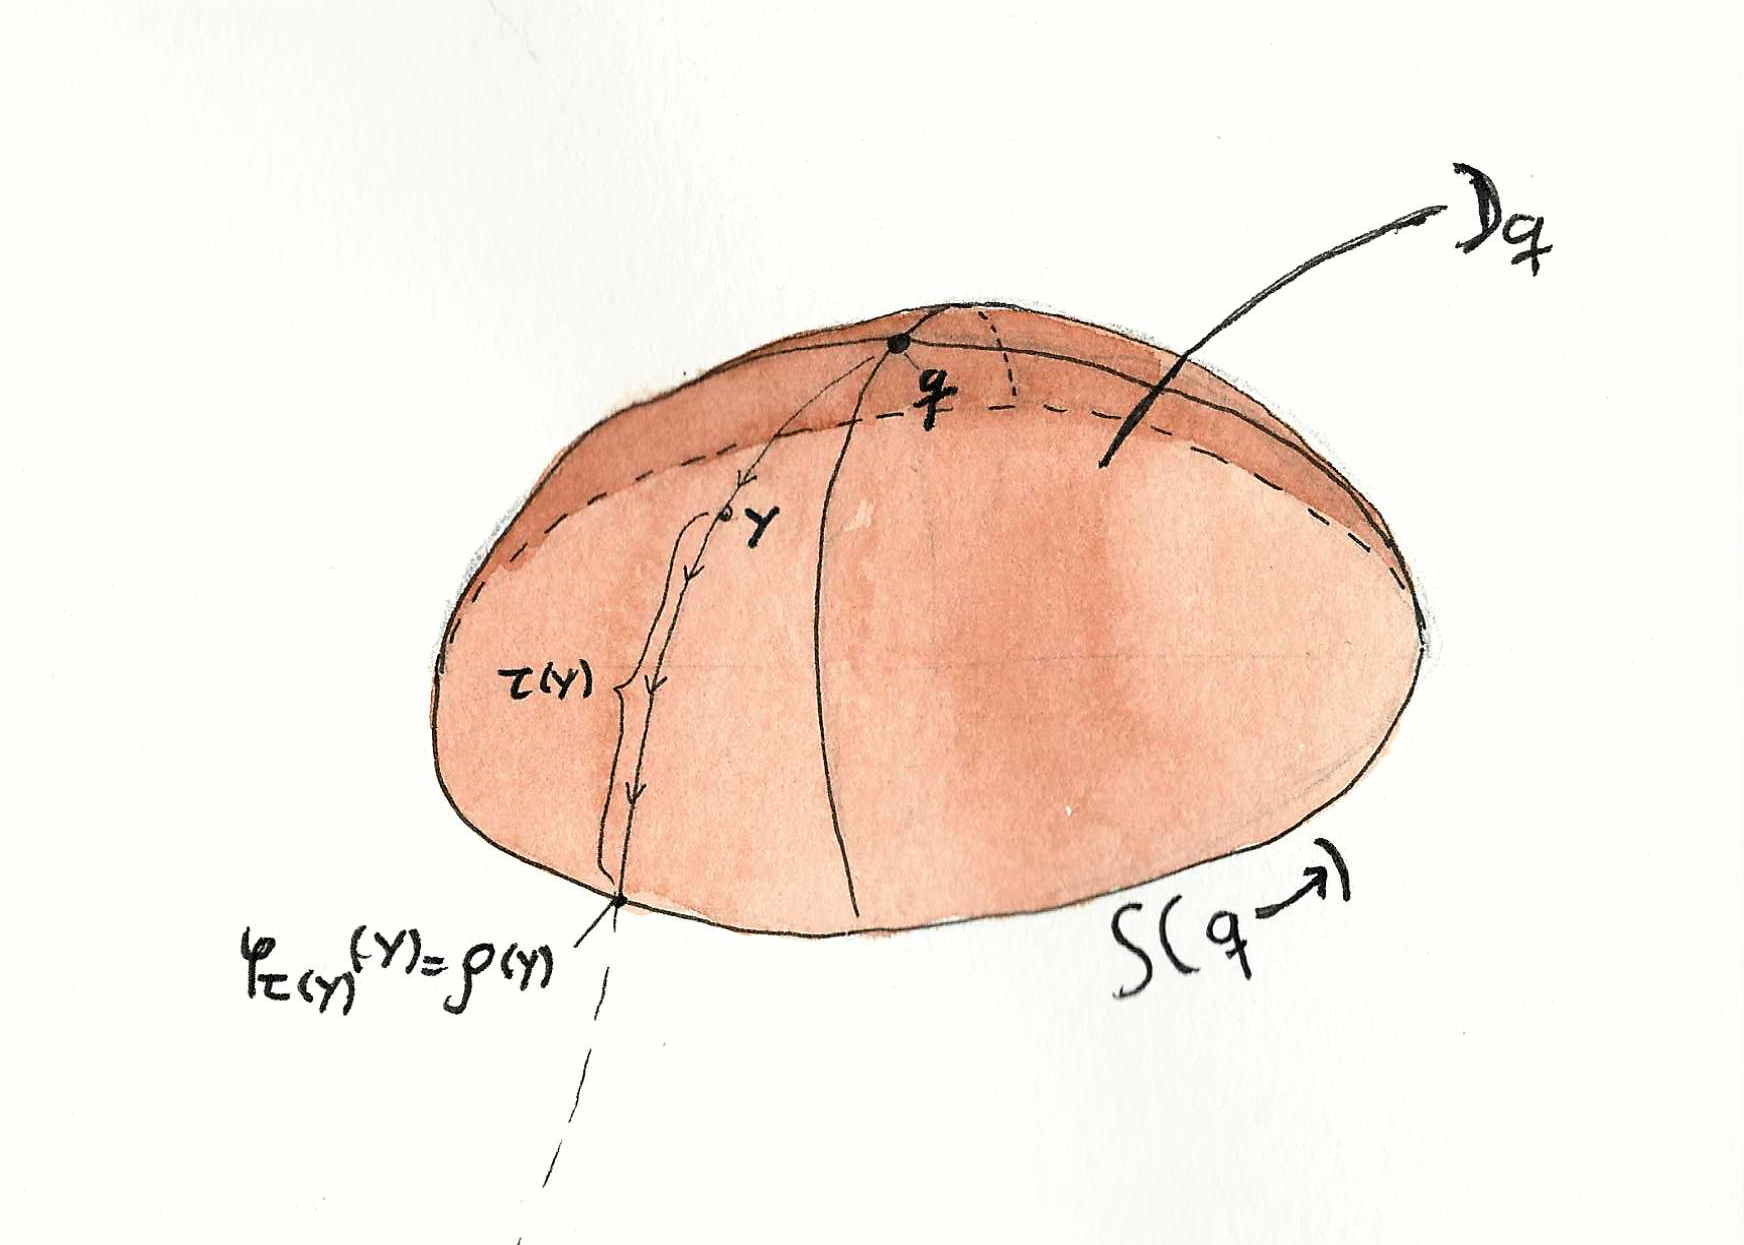
\includegraphics[width=0.49\textwidth]{text/images/TauAndRho.jpg}
	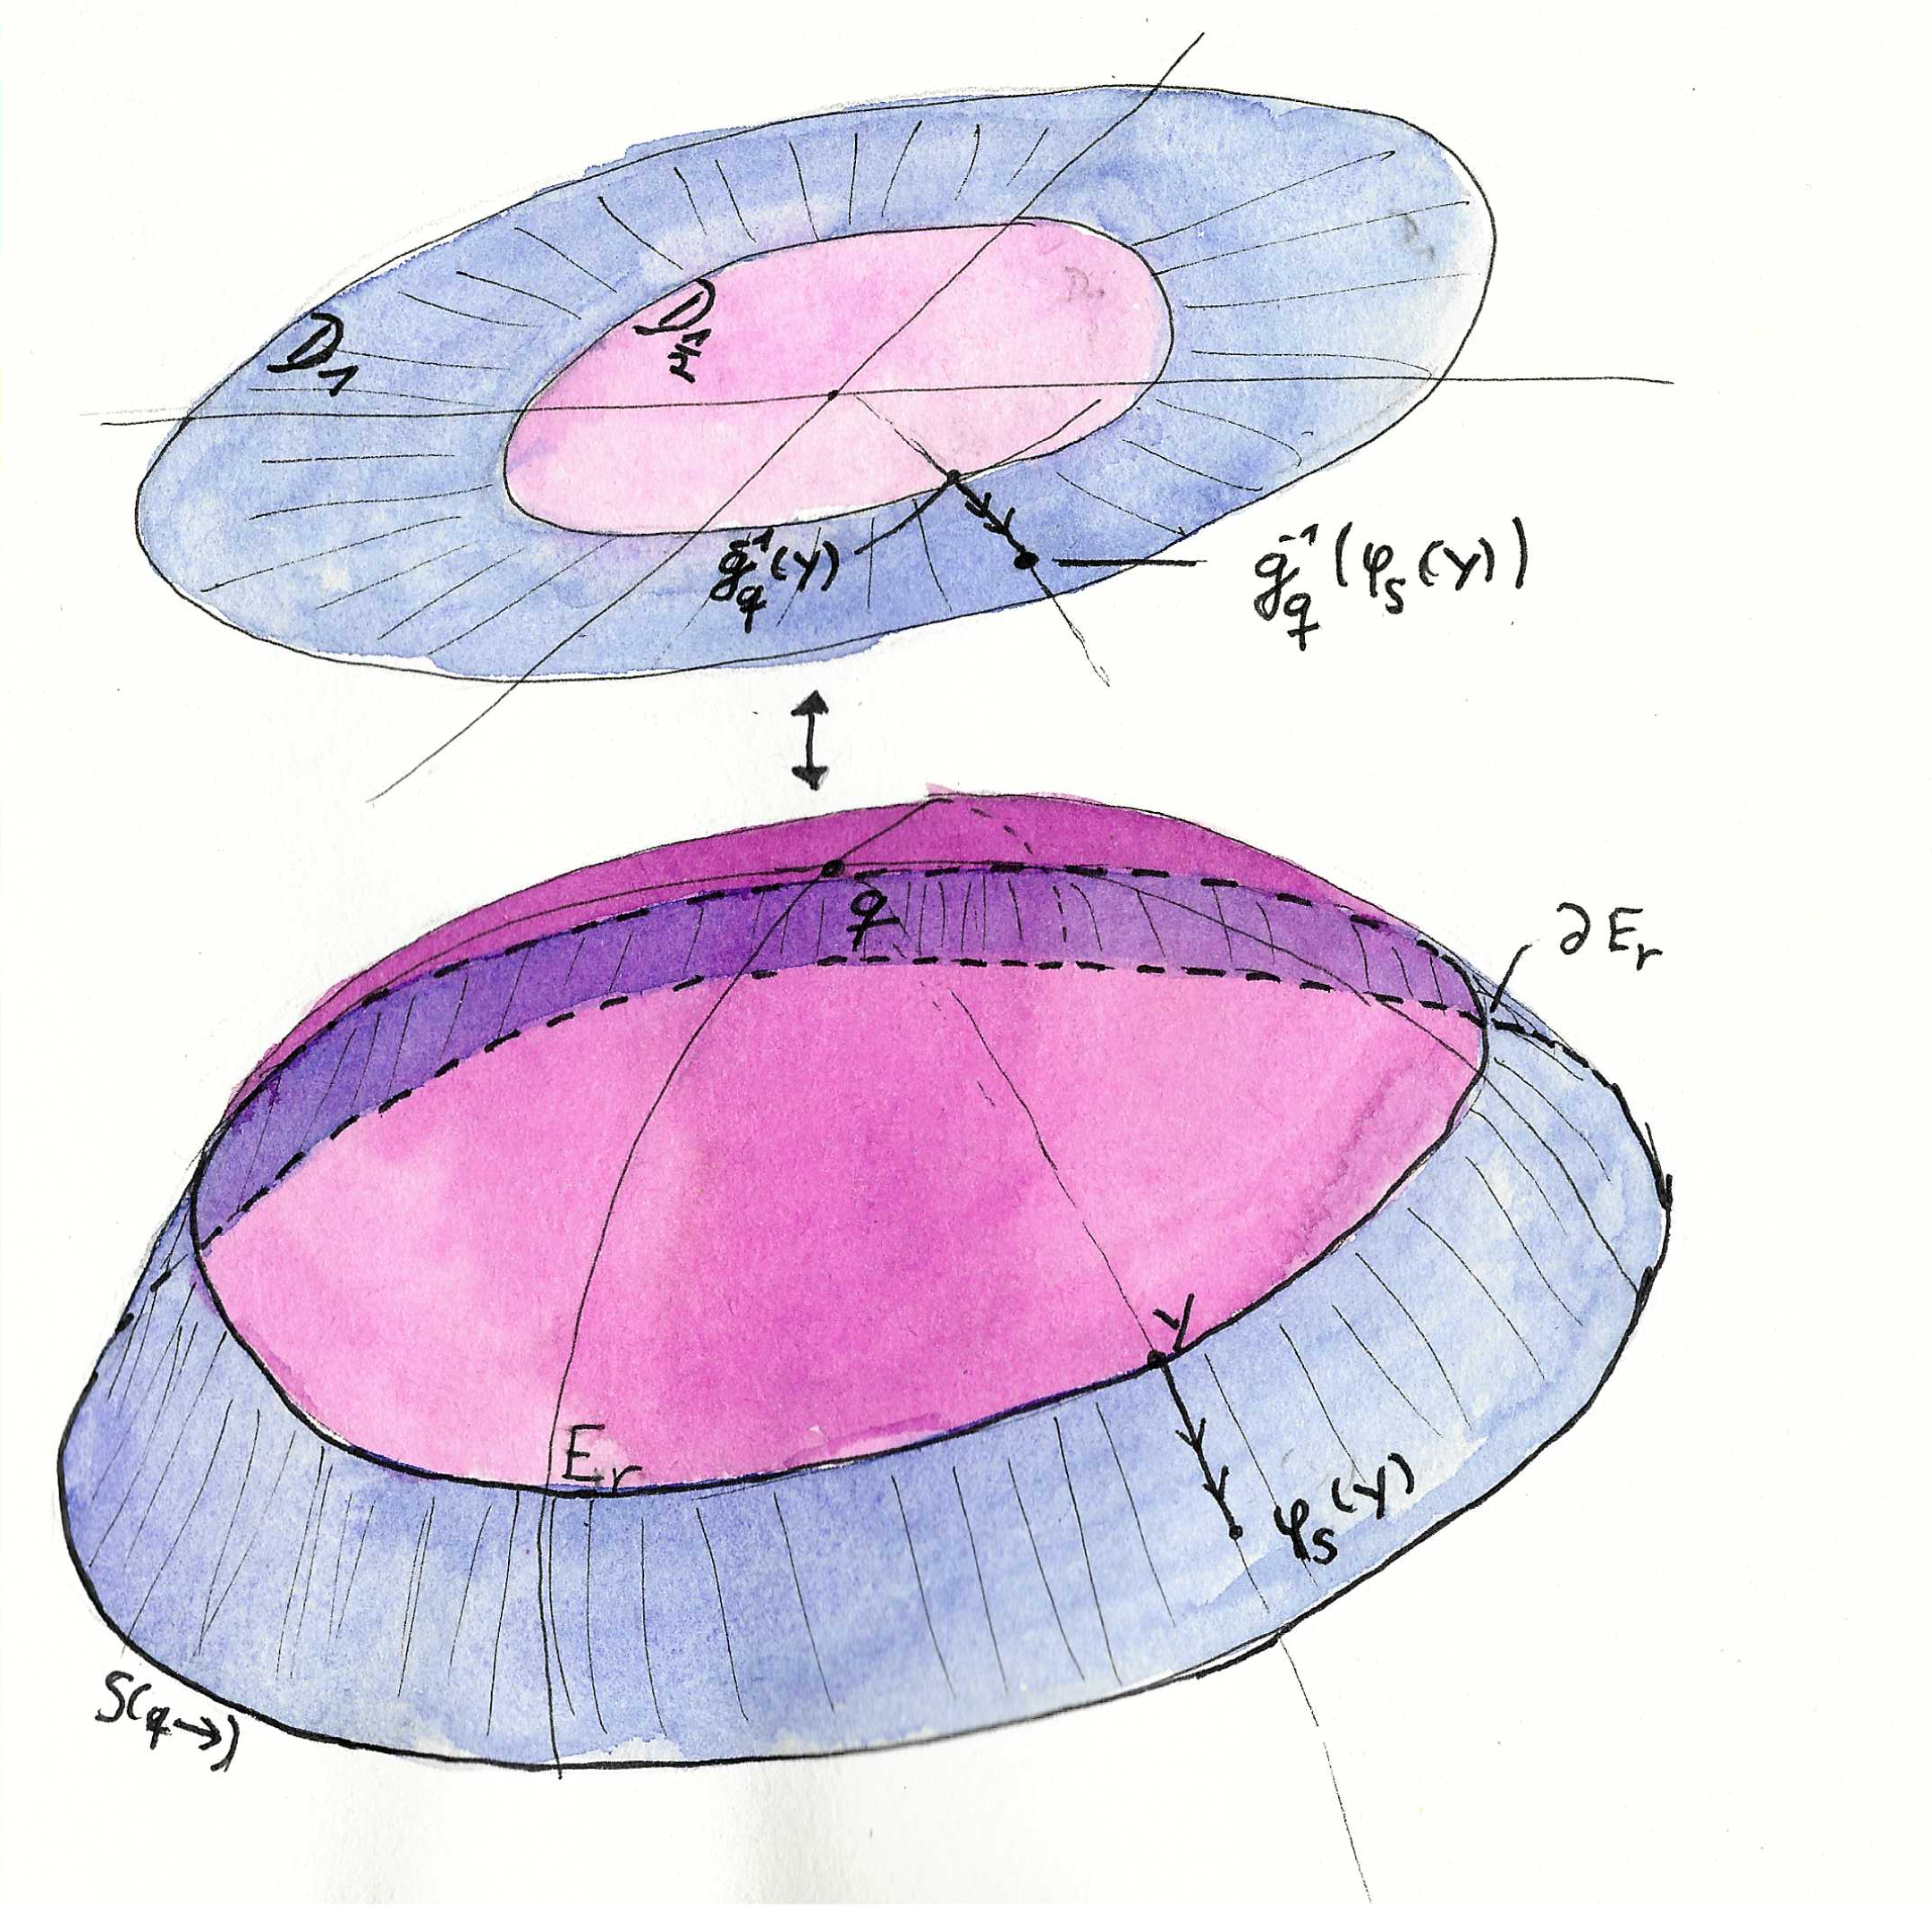
\includegraphics[width=0.49\textwidth]{text/images/theMapGinQ.jpg}
	\caption{The map $\tau$ and $\rho$ from Lemma \ref{lem:morseFilt-flowTimeAndProjectionToLevelSets} (a) is shown on the left and the map $G$ from (c) is shown on the right.}
\end{figure}

\begin{lemma}\label{lem:morseFilt-flowTimeAndProjectionToLevelSets}
	Let $\ind_q(f)\geq1$.
	\begin{enumerate}[(a)]
		\item For $x\in D_q\setminus \{q\}$ there is a unique $\tau(x)\geq 0$ with $\ell(\phi_{\tau(x)}(x))=c$. The resulting map $\tau:D_q\setminus \{q\}\to [0,\infty)$ is smooth, $\tau^{-1}(0)=S(q\to)$, $\tau(\phi_s(x))=\tau(x)-s$, $\restr{\diff \tau}{x}(-\grad_x(f))=-1$ and $\tau(x)\to \infty$ for $x\to q$. We set $\tau(q)=\infty$. 
		\item The map $\rho: D_q\setminus \{q\}\to S(q\to),~\rho(x)\coloneq \phi_{\tau(x)}(x)$ is a smooth retraction with $\rho\circ \phi_s=\rho$. In particular, $\restr{\diff \rho}{x}(\grad_x(f))=0$ and for $y\in S(q\to),~w\in T_y(S(q\to))$ and $s\geq 0$:
		 \begin{equation*}
			\diff \rho \big(\restr{\diff \phi_{-s}}{y}w\big)=w,\quad \diff \tau \big(\restr{\diff \phi_{-s}}{y}w\big)=0\,.
		\end{equation*}
		\item $S(q\to)$ is a closed submanifold of $W(q\to)$ of dimension $\ind_q-1$. There are homeomorphisms $g_q:S^{\ind_q} \to D_q /S(q\to) $ with $g_q(S)=[S(q\to)]$ and a constant $T_q\geq 0$ such that, with the open neighbourhood 
		\begin{equation*}
			W_q\coloneq \{x\in D_q \mid \tau(x)>T_q\}\ni q
		\end{equation*} of $q$, the map $g_q$ restricts to an orientation preserving diffeomorphism from $U_q\coloneq g_q^{-1}(W_q)$ onto $W_q$. 
	\end{enumerate}
\end{lemma}\todo{Bild}

\begin{proof}
(a) Every flow line in $W(q\to)\setminus \{q\}$ has to end in a critical point of index $<k$, where $\ell\leq k-1$. Thereby the flow line needs to pass through $\ell^{-1}(c)$ which is between $k-1$ and $k$. Since $\ell$ strictly decreases along flow lines (ouside of critical points), the flow line passes through $\ell^{-1}(c)$ exactly once.
 
The smoothness follows from the implicit function theorem applied to $G(x,t)\coloneq \ell(\phi_t(x))-c$, since $\partial_t G(x,t)=\diff \ell (-\grad(f))\neq 0$ (by definition of $\ell$). Differentiating $\tau(\phi_s(x))=\tau(x)-s$ in $s=0$ gives $\diff \tau (-\grad(f))=-1$. Finally assume that $x_n\to q$ whilst $\tau(x_n)\leq T$ for some $T>0$. Then we can pass to a subsequence such that $\tau(x_n)\to t$ for $t\leq T$. In this subsequence we then have that $\lim_{n\to \infty}\ell(\phi_{\tau(x_n)}(x_n))=\ell(\phi_t(q))=k$ contradicting $\ell\big(\phi_{\tau(x_n)}(x_n)\big)=c<k$ for all $n\in \N$. 

(b) By (a) we have that $\rho\circ \phi_s=\rho$, and differentiating it in $s$ gives us $\diff \rho (\grad(f))=0$. The last two identities are the differentials of $\rho\circ \phi_{-s}=\id$ and $\tau \circ \phi_{-s} =\mathrm{const}_s$ on $S(q\to)$.

(c) $\grad(f)$ is tangent to $W(q\to)$ (meaning that it is contained in the tangent bundle of $W(q\to)$ as a subbundle of $TM$) and non-zero away from $q$. Hence, $c$ is a regular value of $\restr{\ell}{W(q\to)}$, ($\diff \restr{\ell}{W(q\to)} (\grad(f))$ is nonzero outside of critical points) hence $S(q\to)$ is a submanifold of $W(q\to)$.

Let $\psi=(\psi_s,\psi_u)$ be a refined Morse chart around $q$ such that the unstable coordinates correspond to a positively oriented basis of $T^u_qM=T_qW(q\to)$. Assume the domain to be small enough such that $\ell=f+\mathrm{const}$, and hence, we have a refinde morse function for $ell$ aswell.
Here, $\psi_u$ denotes $\pi_u\circ \psi$ where $\pi_u$ projects to the unstable coordinates (and $\pi_s$ is defined analogously). 
By Lemma \ref{lem:morse-localUnStableManifoldTheorem} the unstable manifold is, in these coordinates the graph of a smooth function $g$ with $g(0)=0$, that is Lipschitz with Lipschitz constant less than one. (This $g$ does not denote the Riemannian metric, which doesnt appear by name in this proof.)
Hence, $\psi_u$ restricts to a diffeomorphism from a neighbourhood $O$ of $q$ in $W(q\to)$ onto an open ball around $0$ and $\norm{\psi(x)}\leq \sqrt{2}\norm{\psi_u(x)}$ on $O$ 
(The latter is deduced from the lipschitz constant of $g$  being less than or equal to one). Write $u(t)\coloneq \psi_u(\phi_t(x))$ for $x\in O$ (and $t$ small enough such that $\phi_t(x)\in O$) and denote pullback of the gradient via the chart $\psi$ by $X\coloneq -q_{\psi}\circ \grad(f)\circ \psi^{-1}$, where $q_\psi$ denotes the coordinate map on the tangent bundle induced by the frame $\partial_i$ (which comes from the morse chart. Compare Definition \ref{def:morse-jacobeanOfTheGradient}). 
By Lemma \ref{lem:morse-jabobianOfTheGradient} together with Remark \ref{rem:morse-jacobianOfTheFlowInRefinedMorsechart} we know that $\restr{\diff X}{0}=J(\grad(f))_{\psi}(0)$ is diagonal. Now we define 
\begin{equation*}
	Y:\R^{\ind_q}\supseteq B \to \R^{\ind_q}\,,\quad v\mapsto Y(v)\coloneq \pi_u \circ (X_{g(v),v})
\end{equation*} and Taylor-expand said function in the origin. By the chain rule and splitting of the tanget space at the origin we get that $Y(v)=\Lambda v+R(v)$ with $\Lambda=\diag(2\mu_1,\dots ,2\mu_{\ind_q})$ and $\norm{R(v)}=o(\norm{v})$.
 Now \begin{equation*}
	\frac{\diff}{\diff t} (u(t))=\pi_u \circ  q_\psi\circ \frac{\diff}{\diff t} \phi_t(x)=\pi_u \circ q_\psi \circ -\grad_{\phi_t(x)}(f)=Y(u(t))\,.
\end{equation*} Thus, with Cauchy-Schwarz we can calculate that for $v$ close enough to zero:

\begin{equation*}
	\frac{\diff}{\diff t}\frac12\norm{u(t)}^2=\big\langle u(t),\Lambda u(t)\big\rangle\underbrace{+\big\langle u(t),R(u(t))\big\rangle}_{\geq -\norm{u(t)}\cdot \underbrace{\norm{R(u(t))}}_{\leq \mu_{min}\norm{u(t)}}}\geq 2\mu_{\min}\norm{u(t)}^2-\mu_{\min}\norm{u(t)}^2>0\,.
\end{equation*} 
Now choose $r$ small enough such that the estimate holds and the ball $B_r(0)\subseteq \psi_u(O)$, and $\ell>c$ on $E_r\coloneq (\restr{\psi_u}{O})^{-1}(B_r(0))$. Then:
\begin{enumerate}[(i)]
	\item For $y\in \partial E_r$ and $t>0$ we have $\phi_{-t}(y)\in \inti(E_r)$, since $\psi_u(\phi_{-t}(y))$ strictly decreases in $t$, by the estimate above.
	\item Every flow line in  $D_q\setminus \{q\}$ meets $\partial E_r$ exactly once: It meets the boundary at least once, as it starts in $q\in \inti(E_r)$ and ends in $S(q\to)$ which is disjoint from $E_r$. If a flow line met the boundary at multiple times, there would be a time $t_0$ where the flow line reenters $E_r$, which forces the $t$ differential of said flow line in the chart $\psi_u$ to be less than or equal to $0$ (the norm needs to be non-increasing), which contradicts the estimate above.
\end{enumerate}

Now we come to the homeomorphism: By (ii), the map 
\begin{equation*}
	\Theta:\{(y,s)\mid y\in \partial E_r, 0\leq s \leq \tau(y)\}\to D_q\setminus \inti(E_r)\,,\quad \Theta(y,s)\coloneq \phi_s(y)
\end{equation*}  is a continuous bijection from a compact set into a Hausdorff space and hence a homeomorphism. Now we define for the unit ball $D_1$:
\begin{align*}
	G:D_q\to D_1\subseteq \R^{\ind_q}\,, \quad 
	\begin{cases}
		G(x)\coloneq \frac{1}{2r}\psi_u(x) & \text{ for }x\in E_r,\\
		G(\phi_s(y))\coloneq \left(\frac12 + \frac{s}{2 \tau(y)}\right) \frac{\psi_u(y)}{r}&\text{ for } y\in \partial E_r,~ 0\leq s\leq \tau(y)\,.
	\end{cases}
\end{align*}
Both formulas define something continuous (even smooth on their domain) and agree on $\partial E_r$. Hence $G$ is continuous. Furthermore, $G$ is bijective and the domain is compact, whilst the image is Hausdorff, giving us a homeomorphism that maps $S(q)$ onto $\partial D_1$. Now let $\overline{\pi_S}:S^{\ind_q}\to \overline{\R^{\ind_q}}$ denote the function from Definition \ref{def:orient-fromRelaSpaceToTheSphere} and with this define 
\begin{equation*}
	g_q^{-1}\coloneq \overline{\pi_S^{-1}}(\frac{G}{1-\norm{G}}): D_q\big/S(q\to) \to S^{\ind_q}
	\quad \text{ where $\frac{x}{0}\coloneq \infty$. for $x\in \R$}
\end{equation*} 

Now only the statement about the orientation preservation of $g_q$ at a neighbourhood of $q$ is missing: Define $T_q\coloneq \max_{\partial E_r}\tau$. If $\tau(x)>T_q$ and $x\neq q$, let $y$ be the point, where the flow line through $x$ passes through the boundary $\partial E_r$. Then $x=\phi_{-t}(y)$ with $t=\tau(x)-\tau(y)>0$ and thereby $x\in \inti(E_r)$ by (i). Hence, $W_q\subseteq \inti (E_r)$ and in said interior of $E_r$ $G$ is a diffeomorphism that is orientation preserving at $q$ by the definition of $\psi_u$ and by Lemma \ref{lem:orient-computingSignInCharts} we know that the sign of the determinant of a diffeomorphism of oriented manifolds is computed by a smooth procedure, and thereby it is locally constant, making $G$ orientation preserving on the whole $\inti(E_r)$. The map $\overline{\pi_S^{-1}}$ is orientation preserving: This follows from the orientation of $S^{\ind_q}$ by Remark \ref{conv:orient-orientationOfTheSphere}. Furthermore, the stretching $v\mapsto \frac{v}{1-\norm{v}}$ is orientation preserving where $D_1$ is oriented as a subspace of $\R^{\ind_q}$(this can be shown by looking at the sign of the determinant of its Jacobian). Hence the whole composition $g_q^{-1}$ is orientation preserving and thereby also $g_q$ is.
\end{proof}
\begin{figure}
	\centering
	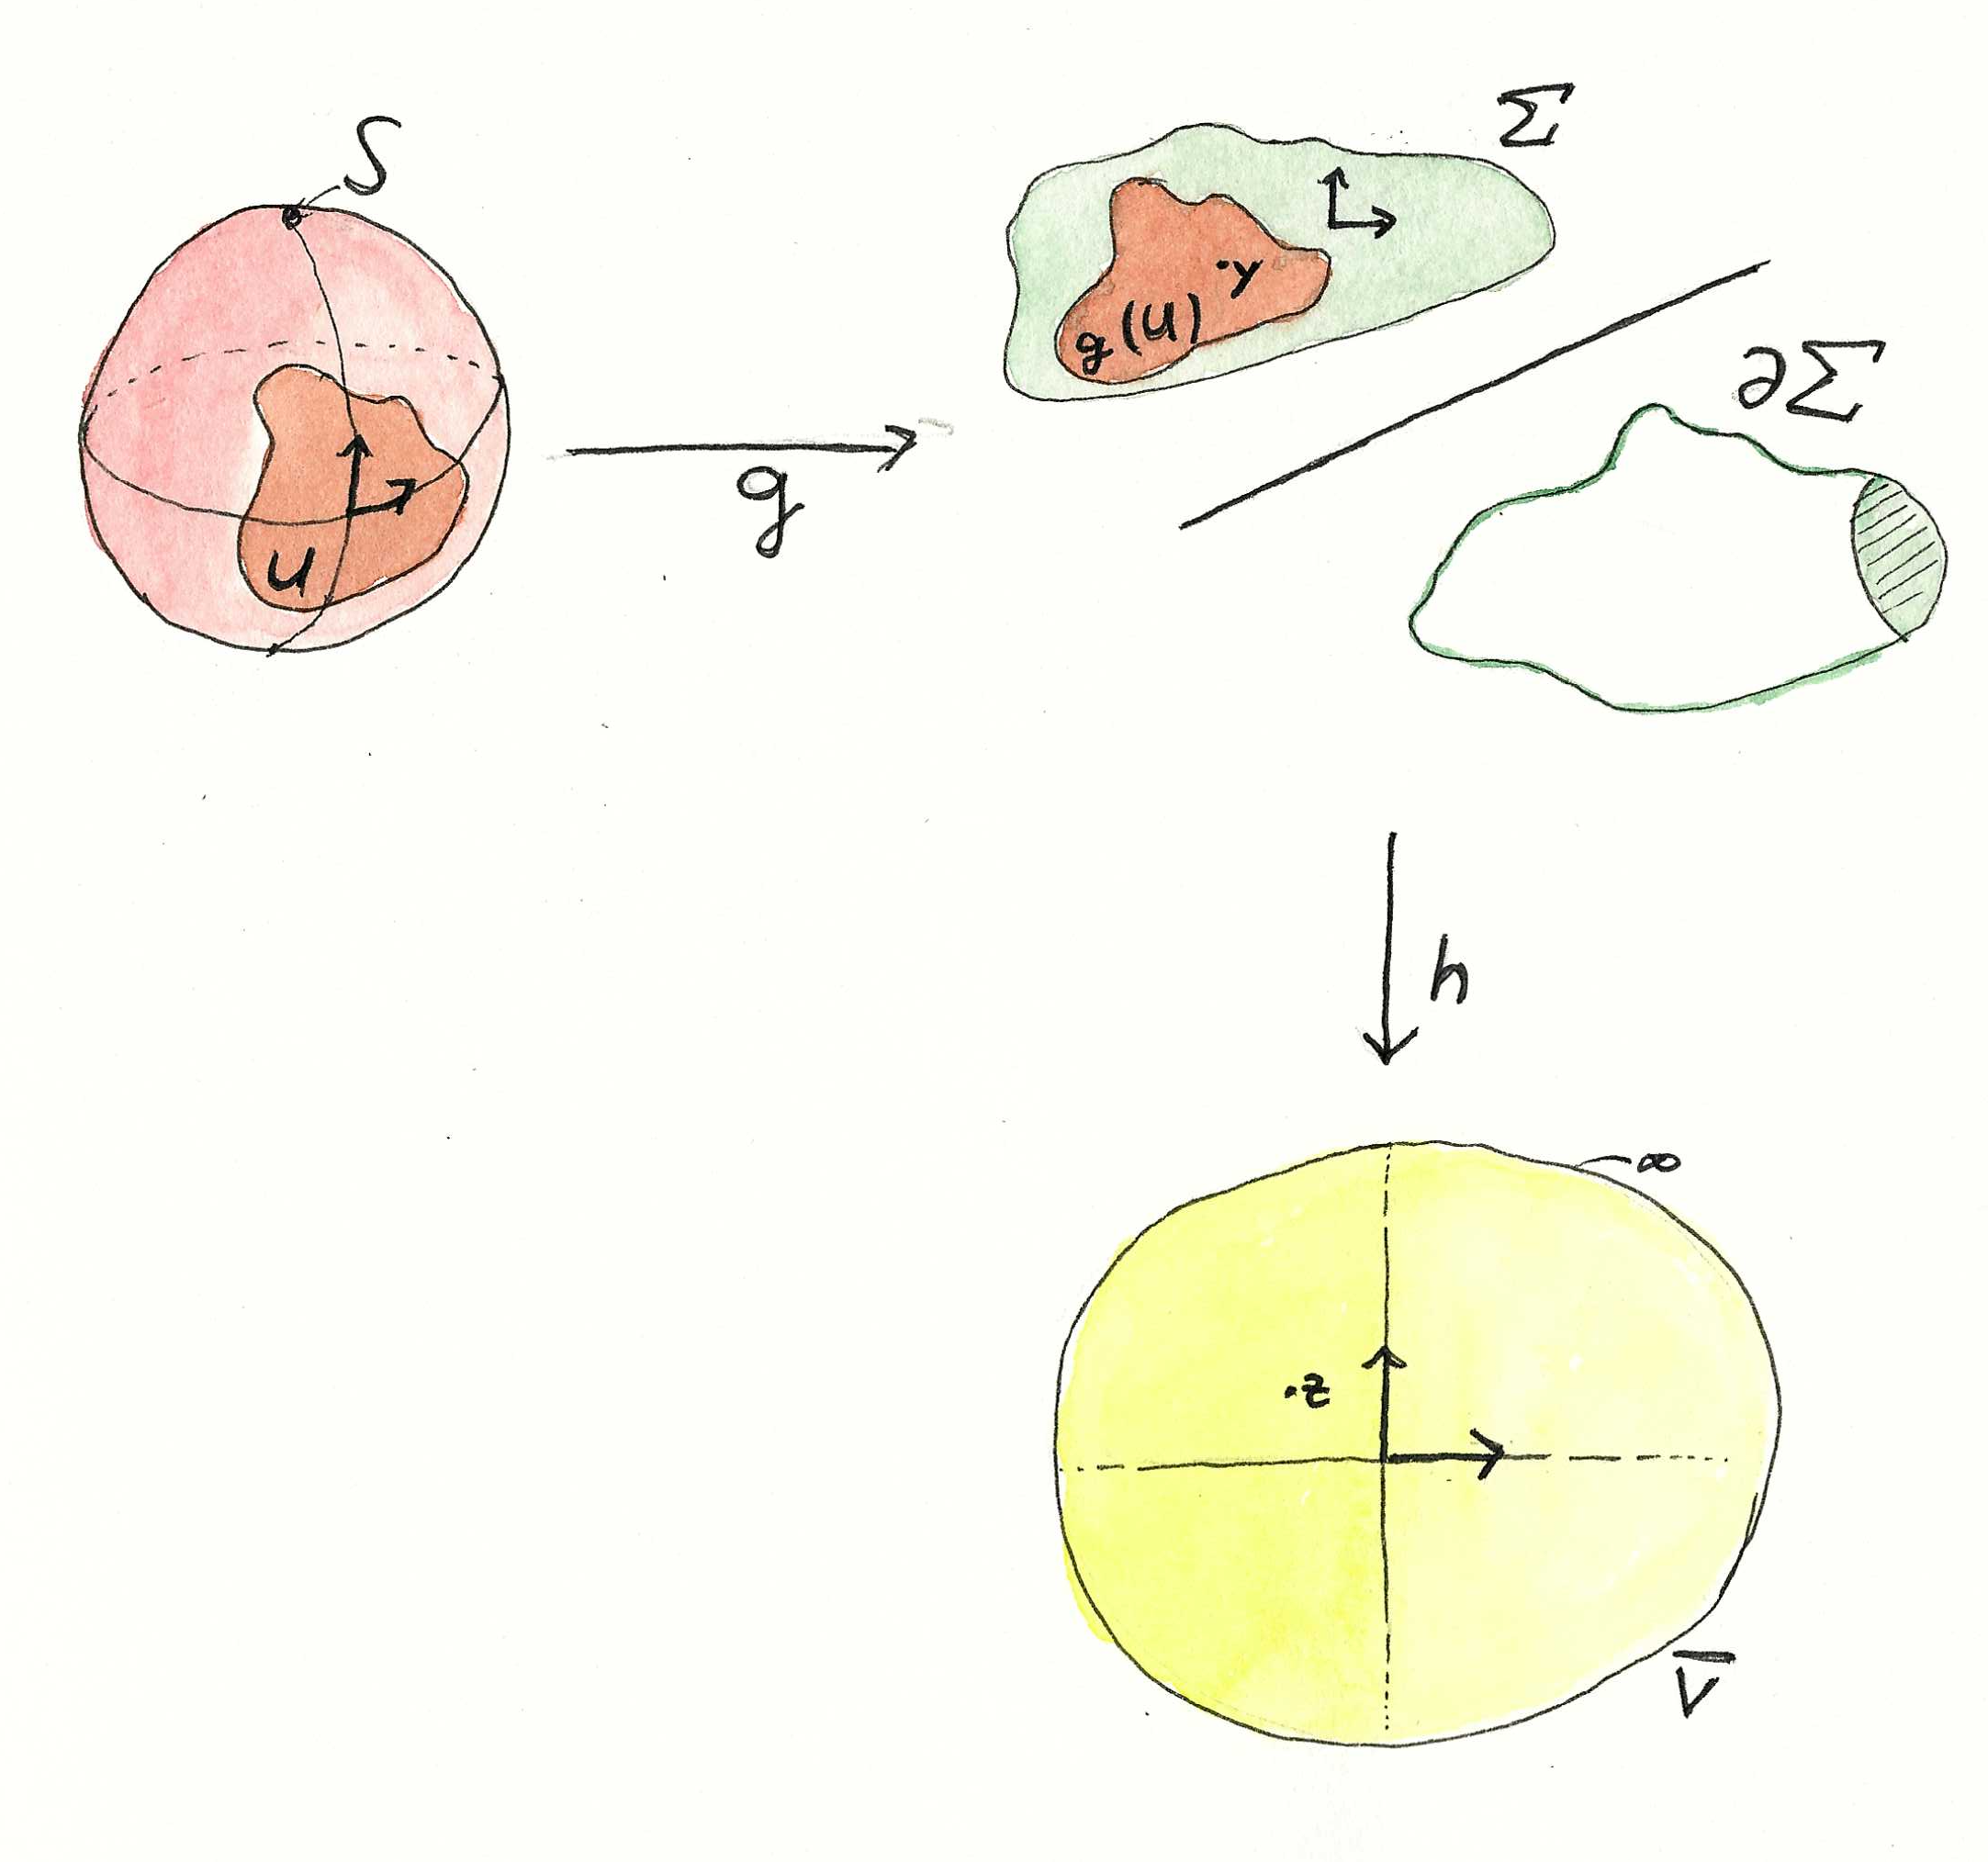
\includegraphics[width=0.6\textwidth]{text/images/InduceOrientationByLinearAndDiffeo.jpg}
	\caption{The setup of Lemma \ref{lem:morseFiltr-orientationClassOfADisk}.}
\end{figure}


\begin{lemma}\label{lem:morseFiltr-orientationClassOfADisk}
	Let $n\geq 1$ and let $(\Sigma,\partial \Sigma)$ be a compact pair ($\partial \Sigma$ denotes a closed subspace of $\Sigma$, and not some kind of boundary. In applications of the Lemma, it will be a boundary) such that $(\Sigma \setminus \partial \Sigma)$ is an oriented $C^1$-manifold of dimension $n$. Let $g:S^n\to \Sigma \big/ \partial \Sigma$ be a homeomorphism with $g(S)=[\partial \Sigma]$ (where $S$ denotes the south pole), and let $U\subseteq S^n\setminus S$ be open such that $\restr{g}{U}$ is an orientation preserving $C^1$-diffeomorphism onto an open subset of $\Sigma \setminus \partial \Sigma$. Define
	\begin{equation*}
		o_{\Sigma}\coloneq (g^{-1})^*(\beta_n)\in\tilde{K}^{-n}(\Sigma /\partial \Sigma)= K^{-n}(\Sigma , \partial \Sigma)\,,
	\end{equation*} with $\beta_n$ being the canonical generator defined in Definition \ref{def:ktheo-higherBottGenerators}. Let $V$ be an oriented $n$-dimensional vector space with K-theoretic orientation $\beta_V$ and $h:\Sigma / \partial \Sigma \to \overline{V}$ be a pointed map such that for some $z\in V$ we have that $h^{-1}(z)=\{y\}$ with $y\in g(U)$, $h$ is $C^1$ near $y$ and $\restr{\diff h}{y}$ is invertible. Then
	\begin{equation*}
		h^*(\beta_V)=\sign\det\left(\restr{\diff h}{y}\right)\cdot o_{\Sigma}
	\end{equation*} 
\end{lemma}
\begin{proof}
	Let $\kappa_V:V\to \R^n$ be the coordinate map of a positively oriented basis, meaning that $\left(\overline{\pi_S^{-1}}\circ \overline{\kappa_V}\right)^*(\beta_n)=\beta_V$ (compare Corollary \ref{cor:orient-vectorspaceOrientationInducesKtheoreticOrientation}). Then $\xi\coloneq \overline{\pi_S^{-1}}\circ \overline{\kappa_V}\circ h \circ g:S^n\to S^n$ satisfies:
	\begin{enumerate}[(i)]
		\item $\xi^{-1}(\pi_S^{-1}\circ \kappa_V(z))=\{g^{-1}(y)\}$,
		\item $\xi$ is $C^1$ near $g^{-1}(y)\in U$, 
		\item by the chain rule, Lemma \ref{lem:orient-computingSignInCharts} and since $\pi_S^{-1}$, $\kappa_V$ and $g$ are orientation preserving we have:
		\begin{equation*}
			\sign \det(\restr{\diff \xi}{g^{-1}(y)})=\sign \det (\restr{\diff h}{y})\,.
		\end{equation*}
	\end{enumerate}
	Hence by the Single Regular Preimage Lemma \ref{lem:orient-singleRegularPreimage} applied to $\xi^*$ we can calculate
	\begin{equation*}
		g^*h^*(\beta_V)=\xi^*(\beta_n)=\sign \det \left(\restr{\diff h}{y}\right)\cdot \beta_n\,.
	\end{equation*} Finally we can apply $(g^{-1})^*$ from the left to finish the proof.
\end{proof}
\begin{corollary}
	Let $g,g':S^n \to \Sigma /\partial \Sigma$ both satisfy the conditions of Lemma \ref{lem:morseFiltr-orientationClassOfADisk} with respect to $U,U'$, and assume 
	$g(U) \cap g(U')\neq \emptyset$. Then $(g^{-1})^*(\beta_n)=({g'}^{-1})^*(\beta_n)$. Hence, $o_\Sigma$ does only depend on the orientation of $\Sigma\setminus \partial \Sigma$. 
\end{corollary}
\begin{proof}
	Let $y\in g(U)\cap g'(U')$ and let $V=\R^n$. Define $h \coloneq \overline{\pi_S} \circ {g'}^{-1}\;:\Sigma / \partial \Sigma\to \overline{\R^n}$ and $z\coloneq h(y)$. Obviously $h^{-1}(z)=\{y\}$ and $h$ is $C^1$ near $y$ with orientation preserving differential. Then Lemma \ref{lem:morseFiltr-orientationClassOfADisk} gives us 
	\begin{equation*}
		({g'}^{-1})^*(\underbrace{\beta_n}_{\overline{\pi_S}^*(\beta_V)})=h^*(\beta_V)=o_{\Sigma}^{\mathrm{w.r.t.} g}=(g^{-1})^*(\beta_n)\,.\qedhere
	\end{equation*}
\end{proof}
 \begin{remark}[Canonical Generators]\label{rem:morseFiltr-canonicalGeneratorsIndependOfChartAndEpsilon}
	Let $\psi$ and $\tilde{\psi}$ be two refined oriented morse charts and $\epsilon,\tilde{\epsilon}>0$ such that the boxes
	\begin{align*}
		(N_q,L_q)&=(\psi^{-1}(D^s_\epsilon \times D^u_\epsilon)\,,\, \psi^{-1}(D^s_\epsilon \times \partial D^u_\epsilon))\quad \text{and}\\
		(\tilde{N_q},\tilde{L_q})&=(\tilde{\psi^{-1}}(D^s_{\tilde{\epsilon}} \times D^u_{\tilde{\epsilon}})\,,\, \tilde{\psi}^{-1}(D^s_{\tilde{\epsilon}} \times \partial D^u_{\tilde{\epsilon}}))\\
	\end{align*} are regular index pairs. Let furthermore 
	\begin{align*}
		\kappa_q\coloneq&  \restr{\diff \psi^{-1}}{0}\circ R_0\circ s\circ \mathrm{pr}_u \circ \psi	\,:\,(\psi^{-1}( D^{s }_\epsilon\times  D^{u }_\epsilon),\psi^{-1}( D^{ s}_\epsilon\times \partial D^{u}_\epsilon))  \to (\overline{T^u_qM},\{\infty\})\quad \text{and}\\
		\tilde{\kappa}_q\coloneq & \restr{\diff \tilde{\psi}^{-1}}{0}\circ R_0\circ \tilde{s}\circ \mathrm{pr}_u \circ \tilde{\psi}	\,:\,(\psi^{-1}( D^{s }_\epsilon\times  D^{u }_\epsilon),\psi^{-1}( D^{ s}_\epsilon\times \partial D^{u}_\epsilon))  \to (\overline{T^u_qM},\{\infty\})\,,
	\end{align*} such that $\alpha_q^{(N_q,L_q)}\coloneq \kappa_q^*(\beta_{T^u_qM})$ is a generator of $\rK^{-\ind(q)}(N_q,L_q)$ and 
	$\tilde{\alpha}_q^{(\tilde{N}_q,\tilde{L}_q)}\coloneq \tilde{\kappa}_q^*(\beta_{T^u_qM})$ is a generator of $\rK^{-\ind(q)}(\tilde{N}_q,\tilde{L}_q)$. Then the induced elements $(\alpha_q^{(N_q,L_q)})_{\#}$ and $(\tilde{\alpha}_q^{(\tilde{N}_q,\tilde{L}_q)})_{\#}$ agree. 
 \end{remark}
 \begin{proof}
	We start by assumeing $\epsilon$ small enough such that in the box $\psi(N_q)$, the image of the unstable manifold $\psi(W(q\to)\cap N_q)$ is the graph of a $C^1$-function $f: D^u_\epsilon\to D^s_\epsilon$. (If $\epsilon$ from the Remark was to big we defined a third index pair in this step. We will later show that the inuced generator of this one agrees with all other.) Now we define $\Sigma \coloneq f(D^u_\epsilon)$ to be oriented, via $T_q\Sigma=T^u_qM$. Let $\partial \Sigma \coloneq \Sigma \cap L_q$. Now let $j:(\Sigma,\partial \Sigma)\to (N_q,L_q)$ be the inclusion. Then we can apply Lemma \ref{lem:morseFiltr-orientationClassOfADisk} to the two maps:
	\begin{equation*}
    	\kappa_q\circ j\,,\quad \tilde{\kappa}_q\circ h\circ j\;:\;\Sigma/\partial\Sigma\to\overline{T^u_qM}\,.
	\end{equation*}

	\begin{itemize}
		\item Restricted to $\Sigma$ the map $pr_u\circ \psi$ is injective with $f(q)=0$. Furthermore, one calculates that $\restr{\diff(\kappa_q\circ j)}{q}=\tfrac{1}{\epsilon}\Idm_{T^u_qM}$.
		\item $\Sigma$ lies in $W^u(q)$, which is flow invariant, and on $\Sigma$ the map $h$ is either the
    flow $\phi_{3t}$ or the collapse. For $\tilde{\epsilon}$ small, $W^u(q)\cap \tilde{N}_q$ is the graph of the local
    unstable manifold in the chart $\tilde{\psi}$, so $\mathrm{pr}_u\circ\tilde{\psi}$ vanishes on it only at $q$.
    Since $\phi_{3t}(x)=q$ if and only if $x=q$, we get $(\tilde{\kappa}_q\circ h\circ j)^{-1}(0)=\{q\}$.
    Near $q$ we have $h=\phi_{3t}$, hence
    $\restr{\diff(\tilde{\kappa}_q\circ h\circ j)}{q}=\tfrac{1}{\tilde{\epsilon}}\,\restr{\diff(\phi_{3t})_q}{T^u_qM}$.
    This has positive determinant, as $\tau\mapsto \restr{\diff(\phi_{3\tau t})_q}{T^u_qM}$, $\tau\in[0,1]$,
    is a path in $\mathrm{GL}(T^u_qM)$ starting at $\Idm$.
	\end{itemize}
	Thereby the Lemma \ref{lem:morseFiltr-orientationClassOfADisk} gives us 
	\begin{equation*}
		j^*\circ \kappa_q^*(\beta_{T^u_qM})=(\kappa_q\circ j)^*(\beta_{T^u_qM})=o_\sigma=(\tilde{\kappa}_q\circ h\circ j)(\beta_{T^u_qM})=j^*\circ h^*\circ \tilde{\kappa}_q^(\beta_{T^u_qM})
	\end{equation*}
	Now $j^*$ is an isomorphism, as it sends the generator $\beta_{T^u_qM}$ to a generator $o_\sigma$, letting us apply its inverse to conclude that $\alpha_q^{(N_q,L_q)}=\kappa_q^*(\beta_{T^u_qM})= h^*\circ \tilde{\kappa}_q^(\beta_{T^u_qM})=h^*(\alpha_q^{(\tilde{N}_q,\tilde{L}_q)})$. Now two induced elements in a canonical isomorphism class agree, if for any group, the corresponding element agrees. Hence, $(\alpha_q^{(N_q,L_q)})_{\#}=(\tilde{\alpha}_q^{(\tilde{N}_q,\tilde{L}_q)})_{\#}\,.$
 \end{proof}



\begin{remark}\label{rem:morseFiltr-orientDQwithGQ}
	We can apply the Lemma above to the pair $(D_q,S(q\to))$ together with $g=g_q$, and $U=U_q$ from Lemma \ref{lem:morseFilt-flowTimeAndProjectionToLevelSets} (c). 
\end{remark}

\begin{definition}\label{def:morseFiltr-defiunitionVj}[Orientation of $V_j$]
	Let $p$ be a critical point of index $k-1$, and $q$ one of index $k$. Then their are only finitely many $x_1,\dots,x_r\in W(q\to p)\cap S(q\to)$. At each $x_j$ we have that $T_{x_j}W(q\to)=T_{x_j}S(q\to)\oplus \langle \grad_{x_j}(f)\rangle_{\R}$ (follows by counting the dimension) and the gradient of $f$ in $x_j$ is contained in $T_{x_j}W(\to p)$. Thereby we can envoke the Morse-Smale condition on $f$ to deduce
	\begin{equation*}
		T_{x_j}S(q\to)\oplus T_{x_j}W(\to p)=T_{x_j}M\,.
	\end{equation*} Thus, the quotient map $T_{x_j}S(q\to)\to Q^p_{x_j}$ is an isomorphism, where $Q^p\coloneq \restr{TM}{W(\to p)}\Big/ TW(\to p)$ is oriented with respect to $T^u_pM$ as in Proposition \ref{prop:morse-orientTheQuotient}. Hence, we get a orientation in each $T_{x_j}S(q\to)$, which lets us orient the open neighbourhood $O_j\subseteq S(q\to)$ of $x_j$. Assume $\chi_j:O_j\to \R^n$ to be a global chart of said neighbourhood that is oriented.\begin{quote}
		Careful! This chart is oriented with respect to the orientation of $T_{x_j}S(q\to)$ that comes from $Q^p$ which is induced by $T^u_pM$ and NOT oriented as a chart    $S(q\to)$ which can be oriented as a boundary of $D_q$ which gets an orientation from $T^u_pM$. In Fact, this difference will give us the sign that induced the morse boundary operator.  
	\end{quote}
	Now assume that $ \delta>0$ is small enough such that the \textbf{closed discs} $V_j\coloneq \chi_j^{-1}(D_\delta)$ are pairwise disjoint and htereby $V_j\cap W(\to p)=\{x_j\}$. Put
	\begin{equation*}
		g_j\coloneq \overline{\chi_j^{-1}}\circ \overline{r_\delta}\circ \overline{\pi_S}:
		S^n \to V_j/\partial V_j\,.
	\end{equation*}($\overline{r_\delta}:\overline{R^n}\to D_\delta /\partial D_\delta$ denotes the map that is induced by the schrinking $r_\delta$ of $\R^n$ to the open disc $D_\delta$). Near the north pole $g_j$ is an orientation preserving diffeomorphism, so $o_{V_j}\coloneq (g_j^{-1})^*(\beta_n)$ is defined and by Corollary \ref{lem:morseFiltr-orientationClassOfADisk}, depends only on the orientation of $V_j$.
	
	Now for any oriented vector space $W$ we define 
    \begin{equation*}
    h_j:\overline{\kappa_V^{-1}}\circ \overline{\pi_S}\circ g_j^{-1}\;:\;  
    V_j/\partial V_j  W  \to     
    \end{equation*}. This map is orientation preserving, as $\overline{\kappa_V^{-1}}$ and $g_j^{-1}$ are and in this setup, we can apply the Lemma \ref{lem:morseFiltr-orientationClassOfADisk} above with $h^{-1}(0)=\{x_j\}$ to conclude that $h^*_j(\beta_V)=o_{V_j}=(g_j^{-1})^*(\beta_n)$.(It is easy to see that $h_j$ is locally a diffeomorphism and $h$ has an invertable differential in the origin.) \todo{ Bildchen?}
\end{definition}


\begin{comment}
\begin{lemma}[Oriented Tubular Embedding]\label{lem:filt-orientedTubularEmbedding}
	Let $B_p\coloneq W(\to p)\cap M^c$ and let $J:D_{\epsilon}(\mathcal{N})\to N_p$ be the tubular embedding from Lemma \ref{lem:morseFilt-npIsTubular}, where $\mathcal{N}\to B_p$ denotes the normal bundle. Now we can orient the normal bundle via the bundle isomorphism $l:\mathcal{N}\to Q^p$  where $Q^p$ denotes the quotient bundle from Definition \ref{def:morseFilt-setupCommutingDiff}(the map is given by including the normal bundle into the tangent bundle and projecting then onto the quotient bundle). Then $J$ can be chosen to be fibrewise orientation preserving, meaning that with the linear identification $R_0:\mathcal{N}_x\to T_0\mathcal{N}_x$ and the projection bundle map $pr: \restr{TM}{W(\to p)\cap M^c}\to Q^p$ we have that for all $x$ the map
	\begin{equation*}
		pr\circ \restr{\diff  J_x}{0}\circ R_0:\mathcal{N}_x\to Q_x^p
	\end{equation*} is orientation preserving.
\end{lemma}
\begin{proof}
	This follows directly from $pr\circ \restr{\diff  J_x}{0}\circ R_0:\mathcal{N}_x\to Q_x^p$ being a bundle isomorphism. Hence it either is orientation preserving in all fibers, or reversing in all fibers (due to the connected base space). If the latter happens, we redefine $J$ by composing it with a map $\rho$ that reflects, say the first coordinate: Here we choose a global orthonormal trivialisation of $\mathcal{N}$ (which exists since the base space $B_p$ is contractible) such that $\rho$ maps the domain of the tubular embedding isomorphically onto itself. 
\end{proof}
\end{comment}


\begin{comment}
\begin{definition}[Orientation of $V_j$]
	Let $x_1,\dots,x_r$ be the points of $S(q\to)\cap W(q\to p)$ (of which there are finitly many as we can rewrite the intersection to be $\bigcup_{\gamma\in \mathcal{M}(q\to p)}\gamma \cap S(q\to)$ now for each $\gamma$ there is only one intersection point and there are only finitly many $\gamma$.\todo{beweis!!}) At each $x_j$ we have $T_{x_j}W(q\to)=T_{x_j}(S(q\to)) \oplus \langle - \grad_{x_j}(f) \rangle_{\R}$ (THis follows by the regular value theorem, as $T_{x_j}(S(q\to))=\ker restr{\diff \ell}{x_j}$ and by definition of $\ell$ we have that $\diff \ell (\grad)\neq 0$ outside of critical points. Hence the gradient is not in $T_{x_j}(S(q\to))$, but it is in $T_{x_j}W(q\to)$. A count of dimension finishes the argument.) On the other hand, $-\grad_{x_j}(f)\in T_{x_j}(W(\to p))$, so the morse-Smale condition gives 
	\begin{equation*}
		T_{x_j}S(q\to)\oplus T_{x_j}W(\to p)=T_{x_j}M\,,
	\end{equation*}making the projection $T_{x_j}(S(q\to))\to Q^p_{x_j}$ an isomomrphism. We now orient $T_{x_j}$
\end{definition}

\begin{remark}\label{rem:morseFilt-OrientVjWithFunctions}
	Let $V_j$ be a fibre of the tubular neighbourhood from Lemma \ref{lem:morseFilt-npIsTubular} that intersects $S(q\to)$ in $x_j$. Now we orient $V_j$ such that the quotient map $T_{x_j}V_j\to (T_{x_j}M)/(T_{x_j}W(\to p)=Q^p_{x_j}$ is orientation preserving. Then $V_j$ is the image of a fiber of the tubular embedding $J:\mathcal{N}^\epsilon \to M$, where $\mathcal{N}^\epsilon$ denotes the tube arround the $0$ section of radius $\epsilon$ in the normal bundle $\mathcal{N}$. Let $r_j$ be the radial map $\mathcal{N_{x_j}}\to \mathcal N_{x_j}^\epsilon$ (the inverse of $v\mapsto (\frac{1}{\epsilon -\norm{v}})$), and let $\mathfrak{p}_j$ be an oriented basis of the normal bundle $\mathcal{N}$. Finally, let $J$ be an oriented Tubular embedding.
	Then we define 
	\begin{equation*}
		g_j\coloneq \overline{J_{x_0}}  \circ \overline{r_j}\circ \overline{\kappa_{\mathfrak{p}_j}}\circ \overline{\pi_S}:S^n\to V_j/\partial V_j\,.
	\end{equation*} 
	 Arround the north pole, the map $g_j$ is a diffeomorphism orientation preserving, as $\overline{\pi_S}$ is, and so is $J_{x_0}\circ r_j\circ \kappa_{\mathfrak{p}_j}$ (which is true by Lemma \ref{lem:filt-orientedTubularEmbedding}). Hence, their compactifications are orientation preserving. Now for any oriented vector space $V$ we define $h_j:\overline{\kappa_V^{-1}}\circ \overline{\pi_S}\circ g_j^{-1}$. in this setup, we can apply the Lemma \ref{lem:morseFiltr-orientationClassOfADisk} above with $h^{-1}(0)=\{x_j\}$ to conclude that $h^*_j(\beta_V)=o_{V_j}=(g_j^{-1})^*(\beta_n)$.(It is easy to see that $h_j$ is locally a diffeomorphism and $h$ as invertable differential in the origin.)
\end{remark}
\end{comment}
\begin{figure}
	\centering
	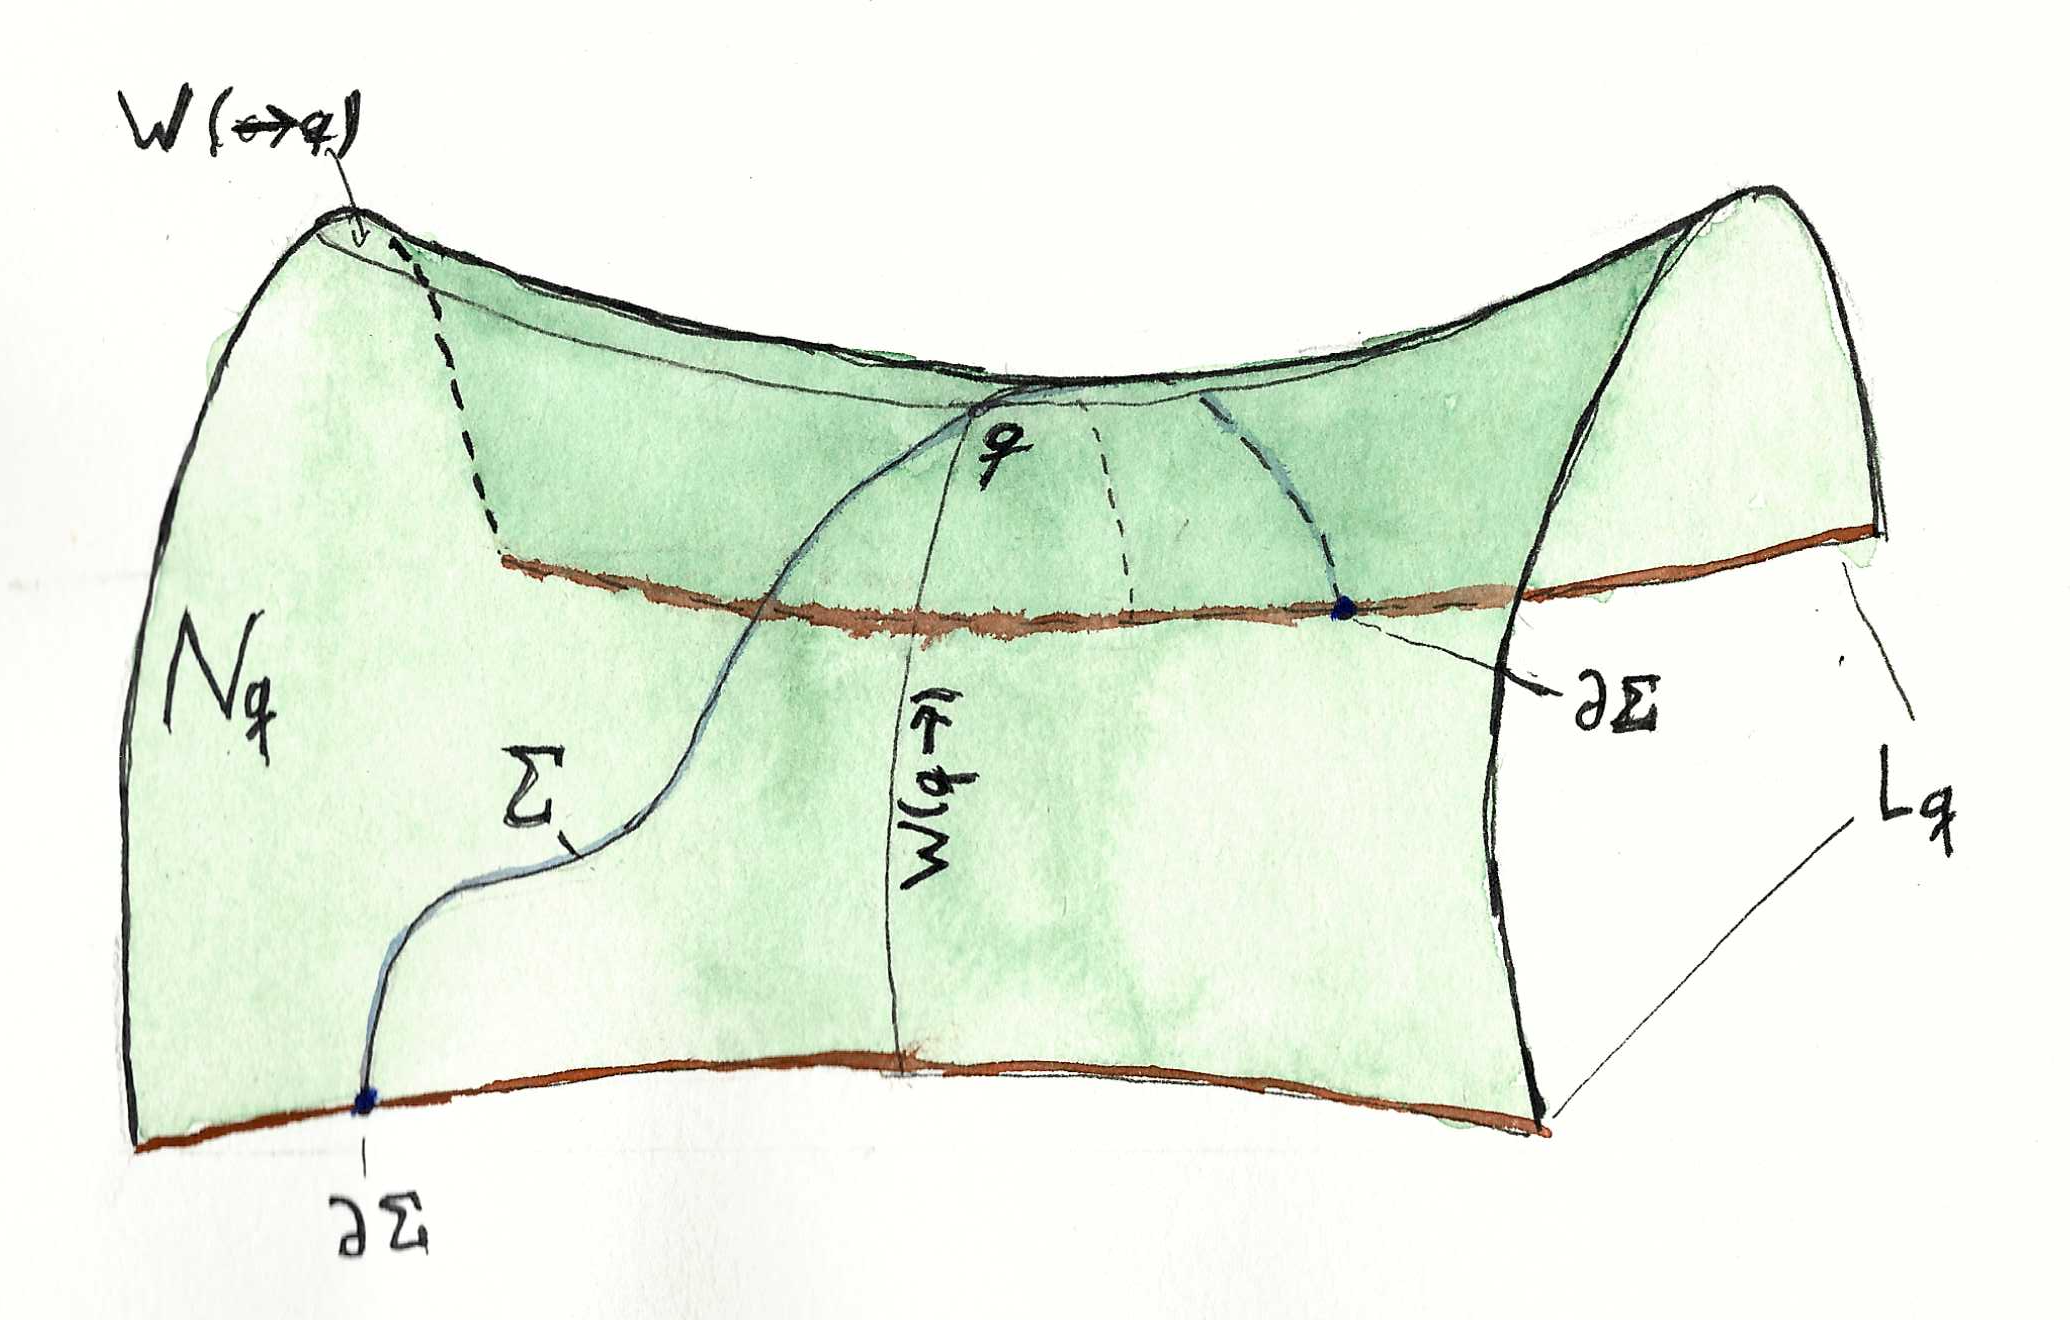
\includegraphics[width=0.7\textwidth]{text/images/induceOrientationsOnTransversDisc.jpg}

	\caption{The definition of the transverse $\Sigma$ from Lemma \ref{lem:morseFilt-canonicalGeneratorsOnTransversalDisks}.}
\end{figure}
\begin{lemma}\label{lem:morseFilt-canonicalGeneratorsOnTransversalDisks}
	Let $q\in \Crit(f)$ with $n\coloneq \ind(q)\geq 1$, let $(N,L)$ be an index pair of $\{q\}$ and let $\Sigma \subseteq N$ with $\partial \Sigma \subseteq L$ be as in Lemma \ref{lem:morseFiltr-orientationClassOfADisk}. Assume 
	\begin{enumerate}[(i)] 
		\item $\Sigma \cap W(\to q)=\{x\}$ with $x\in g(U)$ and $T_x\Sigma \oplus T_xW(\to q)=T_xM$, ($\Sigma$ is transversal)
		\item for every $s\geq 0$ there is a neighbourhood $U_s$ of $x$ in $\Sigma$ with $\phi_{[0,s]}(U_s)\subseteq N\setminus L$.
	\end{enumerate}
	Orient $\Sigma\setminus \partial \Sigma$ such that the isomorphism $T_x\Sigma \to Q_x^q$ is orientation preserving. Then for the inclusion $i:(\Sigma,\partial \Sigma)\to (N,L)$
	\begin{equation*}
		i^*\left(\alpha_q^{(N,L)}\right)=o_{\Sigma}\,.
	\end{equation*}
\end{lemma}

	

\begin{comment}
\begin{remark}
	The two cases where we apply said lemma are: 
	\begin{enumerate}
		\item $\Sigma=D_q,~x=q,~(N,L)=(C,B)$ (from Lemma \ref{lem:morseFilt-flowTimeAndProjectionToLevelSets}) where $Q^q_q=T_qM/T^s_qM\cong T^u_qM$, so $o_{D_q}$ is taken with respect to the orientation of $T^u_qM$. 
		\item $\Sigma=V_j$ $x=x_j$ and $(N,L)=(B,A)$.
	\end{enumerate}
\end{remark}
\end{comment}
\begin{proof}[Proof of Lemma \ref{lem:morseFilt-canonicalGeneratorsOnTransversalDisks}]
	We prove the Lemma in three steps. First we restriced the statement to the easier case, where $\Sigma\subseteq W(q\to)$. Then we define a new chart such that the stable manifold is not just a graph of a function, but a linear subspace. This makes sure that the projection onto the unstable coordinates collapses the stable part to a point which finally in step 3 generalizes the statement for arbitrary $\Sigma$:

	\textit{Step 1}. Let $\chi=(\chi_s,\chi_u)$ be a chart around $q$ such that 
	
	\begin{enumerate}
		\item $W(q\to)$ is the graph of function over the unstable coordinates,
		\item the box $(N_\chi,L_\chi)$ defined as 
	\begin{equation*}
		(\chi^{-1}(D^s_{\epsilon}\times D^u_{\epsilon}), \chi^{-1}(D^s_{\epsilon}\times \partial D^u_{\epsilon}))
	\end{equation*} is a regular index pair of $\{q\}$.
		\item $\epsilon$ is small enough such that $W(q\to)\cap N_\chi$ is the graph of the function from above.
		\item $\diff \chi_q=\diff \psi_q$ where $\psi$ is a refined Morse chart.
	\end{enumerate}
	 The existence of such a chart follows from the local unstable manifold theorem \ref{lem:morse-localUnStableManifoldTheorem}.Let  $\kappa_{\chi}$ be the map defined as 
	 \begin{equation*}
		\kappa_{\chi} \coloneq  \restr{\diff \chi^{-1}}{0}\circ R_0\circ s\circ \mathrm{pr}_u\circ \chi
	 \end{equation*} similar to the construction of $\kappa_q$ in Remark \ref{rem:morseFiltr-morphismToCanonicalIntegers}. Let $\Sigma$ be a disk contained in $W(q\to)$ and hence $\Sigma \cap W(\to q)=q$. Near $q$ and for large $t>0$ the homotopy equivalence $c:(N,L) \to (N_\chi,L_\chi)$ is given by $y\mapsto[\phi_{3t}(y)]$(Compare Theorem \ref{thm:morseFiltr-homotopyEquivalenceOfIndexPairs} and notice that $q$ is in the interior of both $(N\setminus L)$ and $(N_\chi\setminus L_\chi$)). Define $i:(\Sigma,\partial \Sigma) \to (N,L)$ to be the inclusion. 
	 Then consider the function 
	 \begin{equation*}
	 h\coloneq \underbrace{\restr{\diff \chi^{-1}}{0}\circ R_0\circ s\circ \mathrm{pr}_u\circ \chi}_{\kappa_\chi}\circ c\circ i: (\Sigma /\partial \Sigma)\to (\overline{T^u_qM})\,
	 \end{equation*} If $h(y)=0$, then $y$ cannot be $[\partial \Sigma]$ as that point end at ionfinity. 
	 By definition of $\kappa_{\chi}$ we know that $\chi\circ c\circ i(y)\in D^s_\epsilon \times \{0\}$. 
	 And since $y\in \Sigma\subseteq W(q\to)$, and $c$ restricts to a map from $W(q\to)$ to $W(q\to)$ (restrictied to the right domain, and image), we know that $\chi\circ c \circ i(y)\in \chi(W(q\to))\cap D^s_\epsilon \times \{0\}$. 
	 Finally, we assumed that $W(q\to)$ was the graph of the unstable coordinates in $\chi$ and hence, there is only one $x\in D^s_\epsilon \times \{0\}\cap \chi(W(q\to))$, which is $(0,0)$. Hence $\phi_{3t}(y)=q$ which is a fixpoint of the flow and thereby, $y=q$ and $0$ has a unique preimage under $h$. Furthermore, $\restr{\diff h}{q}$ is an endomorphism on $T^u_qM$. We can calculate its determinant by calculating the jacobean determinants of $c\circ i$ and $\kappa_\chi$ in $q$ (resp. in the origin) in a refined Morse chart seperately: 
	 \begin{enumerate}
		\item The function $\restr{\diff (c\circ i)}{q}$ (restricted in its image to $T^u_qM$) has positive determinant which follows from the flow in a refined morse chart in a critical point restricted to the unstable space has a differential that is diagonal with positive entries. This was calculated in Remark \ref{rem:morse-jacobianOfTheFlowInRefinedMorsechart}.
		\item The function $\kappa_\chi$ can be differentiated in $q$:
		\begin{equation*}
			\diff \kappa_{\chi}=\diff \Big(\restr{\diff \chi^{-1}}{0}\circ R_0\circ s\circ \mathrm{pr}_u\circ \chi \Big)\,
		\end{equation*}
		 where $\iota\coloneq\restr{\diff\chi^{-1}}{0}\circ R_0:\{0\}\times\R^{n}\to T^u_qM$ is a linear isomorphism (since $\restr{\diff\chi}{q}$ maps $T^u_qM$ onto the unstable coordinate plane) and $s$ is the radial stretching with $\restr{\diff s}{0}=\lambda \id$, where $\lambda>0$. On $T^u_qM$ the map $\mathrm{pr}_u\circ\restr{\diff\chi}{q}$ is the inverse of $\iota$, so, identifying $T_0T^u_qM$ with $T^u_qM$,
\begin{equation*}
	\restr{\diff h}{q}=\lambda\,\restr{\diff\phi_{3t}}{q}\Big|_{T^u_qM}\in\operatorname{End}(T^u_qM)\,.
\end{equation*}
Its determinant is again positive, as the flow restricted to the unstable tangent space of a critical point is diagonal with positive entries.
	 \end{enumerate}
Hence, $\restr{\diff h}{q}$ has positive determinant and Lemma \ref{lem:morseFiltr-orientationClassOfADisk} gives us the equality
\begin{equation*}
	i^*\circ c^*\circ \kappa_{\chi}^*(\beta_{T^u_qM})=h^*(\beta_{T^u_qM})=o_{\Sigma}\,.
\end{equation*} This concludes the proof for the special case, where $\Sigma$ is contained in $(q\to)$.

So far we have seen that for any chart $\chi$ that satisfies the properties from Step 1 there is the equality above. If we choose $\chi$ to be a refined morse chart, then $\kappa_{\chi}^*(\beta_{T^u_qM})=\alpha_q^{(N_\chi,L_chi)}$ is a canonical generator and a member of $(\alpha_q)_{\#}$.

\textit{Step 2} We know by the local unstable manifold theorem, that for our refined morse chart $\psi$ there exists a smooth $g_s$ such that $\psi \big(W(\to q)\big)$ is the graph of $g_s$ with $g_s(0)=0$ and $\restr{\diff g_s }{0}=0$. The chart $\tilde{\psi}\coloneq (\psi_s,\psi_u-g_s\circ \psi_s)$ satisfies $\restr{\diff \tilde{\psi}}{q}=\restr{\diff \psi}{q}$, $W(\to q)=\tilde{\psi}^{-1}(\R^{m-n}\times \{0\})$ (locally), $W(q\to)$ is still the graph of a function over the unstable coordinates and by Remark \ref{rem:morseFiltr-indexPairForDifferentChart} ,for small $\epsilon$, its box $(N_{\tilde{\psi}},L_{\tilde{\psi}})$ is an index pair. We claim now, that $\kappa_{\tilde{\psi}}^*(\beta_{T^u_qM})$ is a member of the canonical generator $(\alpha_q)_{\#}$.
Let $E\coloneq W(q\to)\cap N_\psi$, be the unstable disk in the box of $\psi$. In the chart $\psi$, $E$ is the graph of a map 
\begin{equation*}
	e:D^u_\epsilon\to D^s_\epsilon 
\end{equation*} \todo{Bild einfügen}  Now we define the deformation homotopy for $t\in[0,1]$
\begin{equation*}
	H_t(l,x)\coloneq \big((1-t)l+te(x),x\big)
\end{equation*} that shows that $(E,\partial E)$ is a strong deformation retract of $(N_\psi,L_\psi)$ onto and hence induces an isomorphism $K^{-n}(N_\psi,L_\psi)\to K^{-n}(E,\partial E)$.
Now we apply Step 1 to the two charts $\chi=\psi$ and $\chi=\tilde{\psi}$ with $\Sigma=E$, and $(N,L)=(N_\psi,L_\psi)$. This tells us that pulling back the canonical generator along both paths in the diagram 
\begin{center}
\begin{tikzcd}
                                      &                                                           & {(N_{\tilde{\psi}},L_{\tilde{\psi}})} \arrow[rd, "\kappa_{\tilde{\psi}}"] &                                  \\
{(E,\partial E)} \arrow[r, "i", hook] & {(N_\psi,L_\psi)} \arrow[ru, "c_1"] \arrow[rd, "c_2\simeq \id"] &                                                                           & {(\overline{T^u_qM},\{\infty\})} \\
                                      &                                                           & {(N_\psi,L_\psi)} \arrow[ru, "\kappa_{\psi}=\kappa_q"']                   &                                 
\end{tikzcd}
\end{center} induce the same $o_E$. Now $c_2\simeq \id$ and the inclusion $i$ induces an isomorphism by the deformation above. Hence, 
\begin{equation*}
	c_1^*\circ \kappa_{\tilde{\psi}}^*(\beta_{T^u_qM})=\kappa_q^*(\beta_{T^u_qM})=\alpha_q^{(N_\psi,L_\psi)}\,.
\end{equation*}

But the canonical generators are compatible with the maps $c$ and $c_1^*$ is an isomorphism, we know that $\alpha_q^{(N_{\tilde{\psi}},L_{\tilde{\psi}})}$ is the unique element with $c_1^*(\alpha_q^{(N_{\tilde{\psi}},L_{\tilde{\psi}})})=\alpha_q^{(N_{{\psi}},L_{{\psi}})}$. Thereby 
\begin{equation*}
	\kappa_{\tilde{\psi}}^*(\beta_{T^u_qM})=\alpha_q^{(N_{\tilde{\psi}},L_{\tilde{\psi}})}\,.
\end{equation*}

\textit{Step 3} Now we assume $\Sigma$ to just satisfy the Lemmas conditions, use again $\tilde{\psi}$ and define the map on the quotients
 \begin{equation*}
	h\coloneq \underbrace{\restr{\diff \tilde{\psi}^{-1}}{0}\circ R_0\circ s\circ \mathrm{pr}_u\circ \tilde{\psi}}_{\kappa_{\tilde{\psi}}}\circ c\circ i
 \end{equation*} with $c:(N,L)\to (N_{\tilde{\psi}},L_{\tilde{\psi}})$ being the canonical homotopy equivalence as in Step 1. If $h(y)=0$, then similar to before, we argue, that $h(y)=0$ means that $\tilde{\psi}\circ c\circ i(y)\in D^s_\epsilon\times \{0\}$ which in turn means that $c(y)=\phi_{3t}(y)\in \tilde{\psi}^{-1}(D^s_\epsilon\times\{0\})$. By definition of $\tilde{\psi}$ we made sure that $W(\to q)\supseteq \tilde{\psi}^{-1}(D^s_\epsilon\times\{0\})$. 
 Thereby, our $y\in \Sigma\cap W(\to q)=\{x\}$ by requirements on $\Sigma$. By (ii) and since $\phi_{[t,3t]}(x)$ are close to $q$ for large $t$ our map $h$ equals $h=\kappa_{\tilde{\psi}}\circ \phi_{3t}$ near $x$. 
 Due to the projection $\mathrm{pr}_u$, $\kappa_{\tilde{\psi}}$ is constant on $W(\to q)$ (for a small enough box), and the flow $\phi_{3t}$ preserves $W(\to q)$. Thereby, the differential factors through the kernel of $\diff( \mathrm{pr}_u \circ \tilde{\psi})_{\phi_{3t}(x)}=T_{\phi_{3t}(x)}W(\to q)$. And since $\Sigma$ intersects $W(\to q)$ transversally  we factor through the composition

 \begin{center}
	\begin{tikzcd}
T_x\Sigma \arrow[r, "\restr{\diff h}{x}"] \arrow[d, "\cong"'] & T^u_qM{}                                                                \\
 Q^q_x \arrow[r, "{[\diff \phi_{3t}]}"]                       &  Q^q_{\phi_{3t}(x)} \arrow[u, "{[\diff \kappa_{\tilde{\psi}}]}"']
\end{tikzcd}
 \end{center}
 \begin{comment}
 \begin{equation*}
	\restr{\diff h}{x}:T_x\Sigma \, \xrightarrow{\cong}\,
	 \, \xrightarrow{[\diff \phi_{3t}]} \, Q^q_{\phi_{3t}(x)} \, \xrightarrow{[\diff \kappa_{\tilde{\psi}}]}  \, T^u_qM \,.
 \end{equation*} 
 
 \end{comment}
 
 
 Now the first isomorphism is orientation preserving, by the choice of orientation on $\Sigma$. 

 Since $\phi_s$ preserves $W(\to q)$, its differential induces a bundle morphism $[\diff\phi_s]:Q^q\to Q^q$ over $\restr{\phi_s}{W(\to q)}$ which is an isomorphism on every fibre. As $W(\to q)$ is connected, by Proposition \ref{def:orient-orientedMorphismOfBundlesEquivalentDef} it suffices to check that $[\diff\phi_s]$ is orientation preserving at a single point. We take $q$: since $\phi_s(q)=q$, the map $[\diff\phi_s]_q$ is an endomorphism of $Q^q_q$, and with respect to the basis $([\partial_i(q)])_i$ given by the unstable coordinate vectors of the refined Morse chart it is diagonal with entries $e^{2\mu_is}>0$ by Remark \ref{rem:morse-jacobianOfTheFlowInRefinedMorsechart}. Hence it has positive determinant, and $[\diff\phi_{3t}]$ is orientation preserving (note $3t>0$).

 Similarly, $\kappa_{\tilde\psi}$ is constant $0$ on the local stable disk $W(\to q)\cap N_{\tilde\psi}$, and its differential induces a bundle morphism $[\diff\kappa_{\tilde\psi}]$ from $\restr{Q^q}{W(\to q)\cap N_{\tilde\psi}}$ to the oriented vector space $T^u_qM$ (a bundle over the point $0$). It is an isomorphism on every fibre, since $\mathrm{pr}_u\circ\restr{\diff\tilde\psi}{y}$ is surjective with kernel $T_yW(\to q)$ and $\tilde\psi_u(y)=0$. The local stable disk is connected, and at $y=q$, under the identification $Q^q_q=T_qM/T^s_qM\cong T^u_qM$ by which $Q^q$ is oriented (Proposition \ref{prop:morse-orientTheQuotient}), $[\diff\kappa_{\tilde\psi}]_q$ is the endomorphism $\lambda\id$ of $T^u_qM$ with $\lambda>0$. Hence $[\diff\kappa_{\tilde\psi}]$ is orientation preserving, and so is the composition $\restr{\diff h}{x}$. 

 Lemma \ref{lem:morseFiltr-orientationClassOfADisk} gives us 
 \begin{equation*}
	o_\Sigma=h^*(\beta_{T^u_qM})=i^*\circ c^* \circ \kappa_{\tilde{\psi}}^*(\beta_{T^u_qM})
 \end{equation*}
 Then, Step 2 gives us that $\kappa_{\tilde{\psi}}^*(\beta_{T^u_qM})=\alpha_q^{(N_{\tilde{\psi}},L_{\tilde{\psi}})}\in (\alpha_q)_{\#}$. Thereby $c^* \circ \kappa_{\tilde{\psi}}^*(\beta_{T^u_qM})=\alpha_q^{(N,L)}$ by definition. This finally concludes the proof.
\end{proof}



\begin{definition}
	Let	$\phi_{l,r}:S^l\wedge S^r\to S^{l+r}$ be the map from Definition \ref{def:ktheo-wedgeOfShoperesIsSphere}.
	Then we define the map 
		\begin{equation*}
			\sigma_n:\tilde{K}^{-n}(Y)\to \tilde{K}^{-n+1}(\Sigma Y)
		\end{equation*}
	given by the identifications
	\begin{equation*}
		\sigma_n: \tilde{K}^{-n}(Y)=\tilde{K}(S^n\wedge Y) \xrightarrow{(\phi_{n-1,1}\wedge\id_Y)^*}\tilde{K}(S^{n-1}\wedge S^1\wedge Y)=\tilde{K}^{-n+1}(\Sigma Y)\,.
	\end{equation*}
\end{definition}
\begin{corollary}
    The map $\sigma_n$ is natural, meaning for any $f:Y\to Y'$ the diagram 
	\begin{center}
		\begin{tikzcd}
			\tilde{K}^{-n}(Y') \arrow[r, "\sigma_n"] \arrow[d, "f^*"] & \tilde{K}^{-n+1}(\Sigma Y') \arrow[d, "\Sigma(f)^*"] \\
			\tilde{K}^{-n}(Y) \arrow[r, "\sigma_n"]                 & \tilde{K}^{-n+1}(\Sigma Y)                        
		\end{tikzcd}
	\end{center} comutes.
\end{corollary}
\begin{proof}
	This follows directly from the definitions. Remember that $\Sigma(f):S^1\wedge Y\to S^1\wedge Y'$ is given by $\id_{S^1}\wedge f$, and \begin{equation*}
		\Sigma(f)^*:\tilde{K}^{-n+1}(\Sigma Y')=\tilde{K}(S^{-n+1}\wedge \Sigma Y')\xrightarrow{(\id_{S^{n-1}}\wedge \id_{S^1} \wedge f)^*} \tilde{K}(S^{-n+1}\wedge \Sigma Y)=\tilde{K}^{-n+1}(\Sigma Y)
	\end{equation*}
	Now there is the obvious equality 
	\begin{equation*}
		(\phi_{n-1,1})\circ (\id_{S^{n-1}}\wedge S^1)=(\id_{S^n})\circ \phi_{n-1,1}
	\end{equation*} That follows from the definition of $\phi_{l,r}=\pi_S^{l+r}\circ \Xi^{-1}\circ (\pi_S^l\wedge \pi_S^r)$ together with the naturality of $\Xi$.
But then we can just calculate
	\begin{align*}
		\Sigma(f)^*\circ \sigma_n=\big((\phi_{n-1,1}\wedge \id_Y)\circ (\id_{S^{n-1}}\wedge \id_{S^1}\wedge f)\big)^*=\big((\id_{S^n}\wedge f)\circ \phi_{n-1,1}\wedge \id_Y\big)^*=\sigma_n\circ f^*
	\end{align*}
\end{proof}





\begin{lemma}[Connecting Homomorphism along a Collar]\label{lem:morseFilt-connectingHomomorphismAlongACollar}
Let $(X,Y)$ be a compact pair and $X$ pointed by $y_0\in Y$. Let $s:X\to [0,1]$ be continuous with $s^{-1}(0)=Y$ and let $r:s^{-1}([0,1))\to Y$ be a continuous retraction. Define, with $S^1=I/\partial I$,	

\begin{equation*}
	\overline{k}:X/Y \to \Sigma Y=S^1\wedge Y\,, \quad
	\overline{k}([z])\coloneq
		\begin{cases}
			[1-s(z),r(z)] &\text{if } s(z)<1\,,\\
			* 			  &\text{if } s(z)=1 \,.
		\end{cases}
\end{equation*}
Then for all $n\geq 1$ the connecting homomorphism $\delta :\tilde{K}^{-n}(Y)\to K^{-n+1}(X,Y)$ of Definition \ref{def:kTheo-connectingHomomorphism} satisfies

\begin{equation*}
	\delta=(-1)^n\cdot \overline{k}^*\circ \sigma_n\,,
\end{equation*} where $\sigma_n\coloneq (\phi_{n-1,1} \wedge \id_Y)^*:\tilde{K}^{-n}(Y)= \tilde{K}(S^n\wedge Y)\to \tilde{K}(S^{n-1}\wedge S^1\wedge Y) \cong \tilde{K}^{-(n-1)}(\Sigma Y)$ is the identification via the map $\phi_{l,r}:S^l\wedge S^r\to S^{l+r}$ from Definition \ref{def:ktheo-wedgeOfShoperesIsSphere} together with the associativity of the wedge product and $\overline{k}^*$ denotes $(\id_{S^{n-1}}\wedge \overline{k})^*$.
\end{lemma}
\begin{proof}
	Let $n=1$. With the notation of Definition \ref{def:kTheo-connectingHomomorphism} let 
	\begin{enumerate}[(i)]
		\item $\overline{m}:X\cup CY \to (X \cup CY )/X\cong CY \big/ Y$
		\item $l:CY \big/ Y\to \Sigma Y\,, $ given by $[y,t]\mapsto [t,y]$ as in Proposition \ref{prop:kTheo-coneIsFunctorAndCYoverYIsRedSuspension}.
		\item $\delta=(\pi^*)^{-1}\circ \overline{m}^* \circ l^*\circ \sigma_1$. This is the same map as in Definition \ref{def:kTheo-connectingHomomorphism}. We split $\theta$ into two parts and moved one part to our definition of $\overline{m}$ (The part that used to be the map $T:(X \cup CY )/(X)\cong CY \big/ Y$) and the second part is our map $l$.
	\end{enumerate} 
	Now for $\mu\in [0,1]$ we define the map $H_\mu:X\cup CY \to \Sigma Y$ by
	\begin{equation*}
		H_\mu([y,t])\coloneq [(1-\mu)t,y] \,\text{ on }CY\,, \quad 
		H_\mu(z)\coloneq [(1-\mu)+\mu s(z),r(z)]\, \text{ on }X
	\end{equation*} (and $*$ if $s(z)=1$). The map $H_\mu$ is well-defined as both formulas agree on $Y$, continuous (for all, and in $\mu$) as $s(z)\to 1, H_\mu(z)\to [\partial I]$ and pointed. Furthermore, $H_0=l\circ \overline{m}$:
	\begin{itemize}
		\item On $X$: $l\circ \overline{m}(x)=*$ and $H_0(x)=[1,r(x)]=*$
		\item On $CY$: $l\circ \overline{m}([y,t])=[t,y]$ and $H_0([y,t])=[t,y]\,,$
	\end{itemize} and 
	$H_1=(R\wedge 1)\circ \overline{k}\circ \pi$ with the Reflection $R(t)=(1-t)$ and the quotient map $\pi: X\cup CY\to X /Y$:
	\begin{itemize}
		\item On $CY$: $(R\wedge 1)\circ \overline{k}\circ \pi ([y,t])=(R\wedge 1)\circ \overline{k}([\underbrace{Y}_{=s^{-1}(0)}])=(R\wedge 1)([1,\underbrace{y'}_{y'\in Y}])=[0,y']=[0,y]=H_1([y,t])$
		\item On $X$: $(R\wedge 1)\circ \overline{k}\circ \pi (x)=(R\wedge 1)[1-s(x),r(x)]=[s(x),r(x)]=H_1(x)\,.$
	\end{itemize}
	Hence, by the homotopy invariance and Corollary \ref{lem:kTheo-inversesInKGivenByHomotopicallyMethods}:
	\begin{equation*}
		\overline{m}^* \circ l^*=\pi^*\circ \overline{k}^*\circ (R\wedge 1)^*=-\pi^*\circ \overline{k}^*\quad \Rightarrow \quad \delta=-\overline{k}^*\circ \sigma_1\,.
	\end{equation*} 
	For $n\geq 2$, $\delta$ is by definition the connecting homomorphism of $(S^{n-1}\wedge X,S^{n-1}\wedge Y)$. Define the map $H'_\mu: (S^{n-1}\wedge X) \cup C(S^{n-1}\wedge Y)\to S^1\wedge S^{n-1}\wedge Y$:

	\begin{equation*}
		H'_\mu([[v,y],t])\coloneq[(1-\mu)t,v,y]\,,\quad 
		H'_\mu([v,x])\coloneq \begin{cases*}
			[(1-\mu)+\mu s (x),v,r(x)]& \text{ if }s(x)<1 \,,\\
			*&\text{ if }s(x)=1\,.
		\end{cases*}
	\end{equation*}
	Similar to $H_\mu$, the map $H'$ is a pointed homotopy from $l\circ \overline{m}$ to $(R\wedge 1)\circ \overline{k_n}\circ \pi$ where 
	\begin{equation*}
		\overline{k_n}:S^{n-1}\wedge (X/Y)\to S^1\wedge S^{n-1}\wedge Y\,,
		[v,x]\mapsto [1-s(x),v,r(x)]\,,
	\end{equation*} so $\delta=-\overline{k_n}^*\circ (\phi_{1,n-1}\wedge \id_Y)^*$. Now $\overline{k_n}=(P\wedge \id_Y)\circ (\id_{S^{n-1}}\wedge \overline{k})$
	 where $P:S^{n-1}\wedge S^1\to S^1 \wedge S^{n-1}$ is given by swapping the factors.
	 Now consider the following commuting diagram
	\begin{center}
		\begin{tikzcd}
			S^{n-1}\wedge S^1 \wedge Y\arrow[r,"~P\wedge \id_Y~"]					\arrow [d,"\phi_{n-1,1}\wedge\id_{Y}"']& S^1\wedge S^{n-1} \wedge Y\arrow[d,"\phi_{1,n-1}\wedge\id_{Y}"]\\
			S^n		\wedge Y		  \arrow[d,"\overline{\pi_S}\wedge\id_{Y}"']	\arrow[r,"B"]& S^n \wedge Y \arrow[d,"\overline{\pi_S}\wedge\id_{Y}"]\\
			\overline{\R^n}\wedge Y\arrow[r,"\overline{A}\wedge \id_Y"]& \overline{\R^n} \wedge Y
		\end{tikzcd}
	\end{center} The middle arrow $B\coloneq (\phi_{1,n-1}\circ P\circ (\phi_{n-1,1})^{-1})\wedge \id_Y$ is given by going around the top and commutes by definition. 
	The bottom square commutes by definition of $A$ together with the naturality of the map $\Xi$ that builds up the $\phi_{l,r}=(\overline{\pi_S^{l+r}})^{-1}\circ \Xi^{-1}\circ (\overline{\pi_S^l}\wedge \overline{\pi_S^r})=(\overline{\pi_S^{l+r}})^{-1}\circ\overline{ (\pi_S^l\times \pi_S^r)}\circ \Xi^{-1}$. (The notation and definition is from Definition \ref{def:ktheo-wedgeOfShoperesIsSphere}) (We omittet the identification of $\R^l\times \R^r=\R^{l+r}$). Now $B=B'\wedge \id_Y$ with 
	\begin{equation*}
		B'\,=\,(\overline{\pi_S^{n}})^{-1}\circ\underbrace{\overline{ (\pi_S^{n-1}\times \pi_S^1)}\circ \Xi^{-1}\circ P \circ \Xi\circ \overline{ (\pi_S^1\times \pi_S^{n-1})}^{-1}}_{A:~~\overline{\R^n}\,\to \, \overline{\R^n}}\circ   (\overline{\pi_S^n})
	\end{equation*}
	 Finally the linear map $A$ is given by moving the last coordinate to the front and hence has determinant $(-1)^{n-1}$.  Hence, by Lemma \ref{lem:orient-linearMapsOnSmashProducts} we conclude that $(\overline{A}\wedge \id_Y)^*=(-1)^{n-1}\cdot \id$. Hence $B^*=(\overline{\pi_S}\wedge \id_Y)^*\circ (-1)^{n-1}\cdot \id\circ {(\overline{\pi_S}\wedge \id_Y)^*}^{-1}=(-1)^{n-1}\cdot \id$, as it is the conjugation of $(\overline{A}\wedge \id_Y)^*$ via an isomorphism (Alternativly one could say that $\pm \id$ commutes with grop homomorphisms). As the top square commutes we have
	\begin{equation*}
		 (P\wedge \id_Y)^*\circ (\phi_{1,n-1}\wedge \id_Y)^*=(-1)^{n-1}(\phi_{n-1,1}\wedge \id_Y)^*\,.
	\end{equation*} 
	
	Putting everything together we conclude that 
	
	\begin{align*}
		\delta 
		&=-\overline{k_n}^*\circ (\phi_{1,n-1}\wedge \id_Y)^* \\
		&=-(\id_{S^{n-1}} \wedge \overline{k})^*\circ \underbrace{(P\wedge \id_Y)^*\circ  (\phi_{1,n-1}\wedge \id_Y)^*}_{=(-1)^{n-1}(\phi_{n-1,1}\wedge \id_Y)^*}\\
		&=(-1)^{n}(\id_{S^{n-1}}\wedge \overline{k})^*\circ \underbrace{(\phi_{n-1,1}\wedge \id_Y)^*}_{\sigma_n}
	\end{align*}

\end{proof}

\begin{lemma}\label{lem:morseFiltr-bottMapOnOrientedSuspension}
	Let $V$ be an oriented real vector space of dimension $n\geq 1$, let $g:(0,1)\to \R$ be an orientation preserving diffeomorphism where $(0,1)$ is oriented as a subspace of $\R$ (e.g. $g(t)\coloneq \tan(\pi(t-\frac{1}{2}))$) and 
	\begin{equation*}
		G_V:\Sigma \overline{V}=S^1\wedge \overline{V}\to \overline{\R\oplus V}\,,
		\quad [t,v]\mapsto (g(t),v)\,.
	\end{equation*} Then $G_V$ is a homeomorphism by Lemma \ref{lem:orient-compactificationOfProduct}. We can orient $\R\oplus V$ by putting $\R$ in front. Let $b=\bottg \boxtimes (-)$ be the Bott map. Then there is an $e_n\in \{\pm 1\}$, depending only on $n$, with 

	\begin{equation*}
		b(\sigma_n(\beta_V))=e_n\cdot G_V^*(\beta_{\R\oplus V})\quad \in \tilde{K}^{-(n+1)}(\Sigma \overline{V})\,,
	\end{equation*}
	 where 
	 $\sigma_n\coloneq (\phi_{n-1,1} \wedge \id_{\overline{V}})^*:\tilde{K}^{-n}(\overline{V})= \tilde{K}(S^n\wedge
	  \overline{V})\to \tilde{K}(S^{n-1}\wedge S^1\wedge \overline{V}) \cong \tilde{K}^{-(n-1)}(\Sigma \overline{V})$ 
	 similar to Lemma \ref{lem:morseFilt-connectingHomomorphismAlongACollar}.
\end{lemma}
\begin{proof}
	Both sides of the equation are generators of $\tilde{K}^{-(n+1)}(\Sigma \overline{V}) \cong \Z$, as isomorphisms map generators to generators and the isomorphism to $\Z$ follows from $\Sigma \overline{V}\simeq S^{n+1}$. Hence both sides agree up to a sign $e(V)$:
	\begin{equation*}
		b(\sigma_n(\beta_V))=e(V) G_V^*(\beta_{\R\oplus V})\quad \in \tilde{K}^{-(n+1)}(\Sigma \overline{V})
	\end{equation*}

	In the notation of Lemma \ref{lem:orient-compactificationOfProduct}, the map $G_V$ is given by $ \Xi^{-1}\circ (\overline{g}\wedge \id_{\overline{V}})$, where $\overline{g}$ is the extension $I/\partial I\to \overline{\R}$ of $g$ with $\overline{g}(\infty)=\infty$.
	Let $A$ be an isomorphism $V\to W$. Then using the naturality of $\Xi$ (we omit its indices) we can conclude that:
	\begin{align*}
		G_W\circ (\id \wedge \overline{A})
		&=\Xi^{-1}\circ (\overline{g}\wedge \id_{\overline{W}})\circ (\id \wedge \overline{A})\\
		&=\overline{({g}\times \id_{{W}})}\circ \Xi^{-1} \circ (\id \wedge \overline{A})\\
		&=\overline{({g}\times \id_{{W}})} \circ \overline{(\id \times A)}\circ \Xi^{-1} \\
		&=\overline{(\id \oplus A)}\circ {\overline{({g}\times \id_V})} \circ \Xi^{-1} \\
		&=\overline{(\id \oplus A)}\circ \underbrace{\Xi^{-1} \circ {(\overline{g}\wedge \overline{\id_{{V}}})}  }_{G_V} 
	\end{align*}

	Now by Corollary \ref{cor:orient-mapsbetweenabstractVectorSpacesOnKOrientations} we know that 
	$\overline{A}^*\beta_W=\sign(\det(A))\beta_V$ and $\overline{\id\oplus A}^*(\beta_{\R\oplus W})=\sign\det(A)\beta _{\R\oplus V}$.
	Now $b$ and $\sigma_n$ are natural, hence commute with topological induced maps:
	\begin{align*}
		(\id\wedge \overline{A})^* \circ b\circ \sigma_n (\beta_W)
		&=b\circ \sigma_n\circ (\overline{A}^*\beta_W)=\sign \det(A) \cdot b\circ \sigma_n (\beta_V)\\
		(\id\wedge \overline{A})^* \circ G_W^*(\beta_{\R\oplus W})
		&=(G_W\circ (\id \wedge \overline{A}))^*\beta_{\R\oplus W}
		=G_V^*\circ\overline{ (\id \oplus {A})}^*\beta_{\R\oplus W}\\
		&=\sign(\det(A))\cdot G_V^*\beta_{\R\oplus V}
	\end{align*}
	We now claim that for fixed $n$ the signs $e(V)$ and $e(W)$ defined above agree (and are thereby independent of the chosen vector space). For this we consider the diagram below, that commutes by the considerations above (naturality of $b$ and $\sigma_n$ and $\Xi$):
\begin{center}
	\begin{tikzcd}
	\rK^{-n}(\overline W) \arrow[r,"b\circ\sigma_n"] \arrow[d,"\overline A^*"'] & \rK^{-(n+1)}(\Sigma\overline W) \arrow[d,"(\id\wedge\overline A)^*"] & \rK^{-(n+1)}(\overline{\R\oplus W}) \arrow[l,"G_W^*"'] \arrow[d,"\overline{\id\oplus A}^*"] \\
	\rK^{-n}(\overline V) \arrow[r,"b\circ\sigma_n"'] & \rK^{-(n+1)}(\Sigma\overline V) & \rK^{-(n+1)}(\overline{\R\oplus V}) \arrow[l,"G_V^*"]
\end{tikzcd}\end{center}
This lets us compute:


\begin{align*}
	(\id \wedge \overline{A})^*\circ (b \circ \sigma_n)(\beta_W)
	&= \sign \det (A)\cdot \underbrace{ b\circ \sigma_n (\beta_V)}_{e(V) G_V^*(\beta_{\R\oplus V}) }\\
	&= e(V) \cdot \underbrace{\sign \det (A)\cdot G_V^*(\beta_{\R\oplus V}) }_{(\id\wedge \overline{A})^* \circ G_W^*(\beta_{\R\oplus W})}\\
	&=e(V) \cdot (\id\wedge \overline{A})^* \circ G_W^*(\beta_{\R\oplus W})
\end{align*} Now applying $((\id \wedge \overline{A})^*)^{-1}$ from the left (which exists as it is induced by a homeomorphism) gives us that the sign $e(V)$ satisfies the definition of $e(W)$ making them equal. Thereby $e(V)$ is independent of $V$ and only depends on $n$ (and potentially $g$). Finally, it is invariant under the choice of orientation preserving diffeomorphism $g$, as any two such maps $g_0$ and $g_1$ are homotopic via the homotopy $(1-s)g_0+sg_1$ that extends to a homotopy of the compactifications. Hence $(G_V)^*$ and thus $e(V)$ do not depend on $g$.
\end{proof}


\begin{remark} \label{rem:morseFilt-calculationOfe}
 Let $e_n$ be the sign from Lemma \ref{lem:morseFiltr-bottMapOnOrientedSuspension}. Then $e_n=(-1)^n$.
\end{remark}
\begin{proof}
	By Lemma \ref{lem:orient-multiplication} we know that $\beta_{\R\oplus V}=\Xi^*(\beta_{\R}\boxtimes \beta_V)$. Now with $G_V=\Xi^{-1}(\overline{g}\wedge \id)$ and by naturality of $\boxtimes$ we have that
	\begin{equation*}
		G^*_V(\beta_{\R\oplus V})=(\overline{g}\wedge \id)^*(\beta_{\R}\boxtimes \beta_V)=(\overline{g}^*\beta_\R)\boxtimes \beta_V =\beta_1\boxtimes \beta_V
	\end{equation*}
	On the other side we have $b \circ \sigma_n(\beta_V)=\beta \boxtimes (\sigma_n(\beta_V))$. Now for any $x\in \rK^{-n}(Y)$ we have
	\begin{equation*}
		\beta \boxtimes \sigma_n(x)=(-1)^n\beta_1 \boxtimes_{1,n} x \,\in\, \rK^{-(n+1)}(\Sigma Y)\,.
	\end{equation*}  As both sides are pullbacks of the same product (in the 0th degree) $\beta\boxtimes_{0,0} x\in \rK(S^1\wedge S^1\wedge S^n\wedge Y)$ via two different maps
	\begin{equation*}
		S^{n+1}\wedge S^1\wedge Y \to S^1\wedge S^1\wedge S^n\wedge Y.
	\end{equation*} By definition, $\sigma_n$ takes the last coordinate of the $S^n$ part and maps it to the $S^1$ part. If we give all the coordinates names the left side acts as
	\begin{align*}
		S^{n+1}\wedge S^1\wedge Y &\to S^1\wedge S^1\wedge S^n\wedge Y \\
		(d_1,\dots d_{n+1},s_1,y)&\mapsto(\underbrace{d_1}_{S^1},\underbrace{d_2}_{S^1},\underbrace{d_3,\dots,d_{n+1},s_1}_{S^{n}},\underbrace{y}_{Y})
	\end{align*} where $d_1$ and $d_2$ correspond to $\beta$. 
	
	The right side is defined in Definition \ref{def:kTheo-lowerExternalProduct} as the reduced external product pulled back along a switch of coordinates that swiches the sphere $S^n$ coming from $x\in \rK(S^n\wedge Y)$ with the sphere $S^1$ corresponding to $\beta_1$, or in our notation:
		\begin{align*}
		S^{n+1}\wedge S^1\wedge Y &\to S^1\wedge S^1\wedge S^n\wedge Y \\
		(d_1,\dots d_{n+1},s_1,y)&\mapsto (\underbrace{d_1}_{S^1},\underbrace{s_1}_{S^1},\underbrace{d_2,d_{n+1}}_{S^n},\underbrace{y}_{Y})
	\end{align*}

	Hence, we can translate $\beta_1 \boxtimes \sigma_n(x)$ into $\beta \boxtimes_{1,n} x$ by pulling back along $P\wedge \id_Y$ , whilst $P$ as a linear map between vector spaces has determinant $(-1)^n$ ( we need to move $s_1$ past $n$ basis vectors corresponding to $d_2,\dots d_{n+1}$), letting us apply Lemma \ref{lem:orient-linearMapsOnSmashProducts} to conclude its pullback is the identity times $(-1)^n$. With $x=\beta_V$ we have that
	\begin{equation*}
		b\circ \sigma_n(\beta_V)=(-1)^n\beta_1\boxtimes \beta_V=(-1)^nG_V^*\beta_{\R\oplus V}
	\end{equation*}
	and hence $e_n=(-1)^n$.
\end{proof}
\begin{lemma}\label{lem:morseFiltr-contributionOfASigleFlowLine}
	Let $n\coloneq \ind_p\geq 1$, $V_j\subseteq S(q\to)$ an oriented transversal disk arround $x_j$ as in Remark \ref{def:morseFiltr-defiunitionVj}, $x_j\in W(q\to p)$ and denote the flow line through $x_j$ by $\gamma_j\in \mathcal{M}(q\to p)$. Let $l_j:S(q\to)\to V_j/\partial V_j$ be the collaps and $\delta$ be the connecting homomorphism of the pair $(D_q,S(q\to))$. Then 
	\begin{equation*}
		b\circ \delta\circ l_j^*(o_{V_j})=e(\gamma_j)o_{D_q}\,,
	\end{equation*} where $o_{D_q}=(g_q^{-1})^*(\beta_{n+1})$ with $g_q:S^{n+1}\to D_q/ S(q\to)$ as in Lemma \ref{lem:morseFilt-flowTimeAndProjectionToLevelSets} (c), and $o_{V_j}=(g_j^{-1})^*(\beta_n)$ as in Remark \ref{def:morseFiltr-defiunitionVj}. Said different, the diagram commutes:
	\begin{center}
		\begin{tikzcd}
\tilde{K}^{-n}(V_j/\partial V_j) \arrow[r,"l_j^*"] \arrow[rrd, "o_{V_j}\mapsto e(\gamma_j)(o_{D_q})"', sloped, pos=0.5] & \tilde{K}^{-n}(S(q\to)) \arrow[r, "\delta"] & {{K}^{-n+1}(D_q,S(q\to))} \arrow[d, "b"] \\
                                                                                        &                                             & {{K}^{-(n+1)}(D_q,S(q\to))}             
\end{tikzcd}
	\end{center}
\end{lemma}

\begin{proof}By Lemma \ref{lem:morseFilt-flowTimeAndProjectionToLevelSets} we know that the map $g_q$ restricts to an orientation preserving diffeomorphism over the set $\{x\in D_q \mid \tau(x)>T_q\}$ for some $T_q\geq 0$. Let $T_0>2T_q$ and define the maps 
	\begin{equation*}
		s:D_q\to [0,1]\,,\quad x\mapsto \min\{\frac{\tau(x)}{T_0},1\}
	\end{equation*}
and 
\begin{equation*}
	r:s^{-1}[0,1)\to S(q\to)\,,\quad x\mapsto \rho(x)\,.
\end{equation*}
Now we consider the vectorspace $Q_{x_j}^p$ and its corresponding generator $o_{V_j}=h_j^*(\beta_{Q_{x_j}^p})$ where $h_j$ is the mapping $(V_j/\partial V_j)\to \overline{Q_{x_j}^p}$ Now we want to calculate the connecting homomorphism along the collar $S(q\to)$ in $D_q$ letting us apply Lemma \ref{lem:morseFilt-connectingHomomorphismAlongACollar}, to the pair with the map $s$ and $r$.
Furthermore, the naturality of $\sigma_n$ and $b$ let us deduce
that
\begin{align}
	b\circ \delta \circ l_j^*\circ h_j^*(\beta_{Q_{x_j}^p})
	&=(-1)^n\cdot b\circ \overline{k}^*\circ \sigma_n \circ l_j^*\circ h_j^*(\beta_{Q_{x_j}^p})\label{eq:morseFiltr-boundaryMorphismInASingleFlowLine}\\
	&=(-1)^n\cdot (\Sigma(h_j\circ l_j)\circ \overline{k})^* \underbrace{b \circ \sigma_n(\beta_{Q_{x_j}^p})}_{=\underbrace{e_n}_{=(-1)^n}\cdot \,G_V^*(\beta_{\R\oplus V})} \notag\\
	&=(\underbrace{G_V\circ \Sigma(h_j\circ l_j)\circ \overline{k}}_{\coloneq F})^*(\beta_{\R\oplus Q_{x_j}^p}) \notag
\end{align}
Now we can calculate $F: D_q\big/S(q\to )\to \overline{R\oplus Q^p_{x_j}}$ explicitly:
\begin{equation*}
	F(z)\mapsto \begin{cases}
		[g(1-s(z)),h_j\circ l_j\circ r(z)]&
        \text{ if }
        \underbrace{s(z)<1}_{\text{condition on } r} 
        \text{ and }\underbrace{s(z)\neq 0}_{\text{condition on } g} \Leftrightarrow 0<\tau(z)<T_0\,,\\
		[R\oplus Q^p_{x_j}]& \text{ else}\,,
	\end{cases}
\end{equation*} where $g$ denotes a orientation preserving diffeomorphism $(0,1)\to \R$. 
Gemoetrically, the map $g(1-s(z))$ increases, as we move towards $S(q\to)$. This is the place, where we make sure to point the first basis vector downward, and builds the geometric bridge to the morse co-boundary map. 
But now $F(z)=0$, if and only if $s(z)=\sfrac{1}{2}$ meaning that $2\tau(z)=T_0$ and $\rho(z)=x_j$ meaning that $F^{-1}(0)=\{\phi_{-\frac{1}{2}T_0}(x_j)\}=\{\hat{x}_j\}$.
 Let $(w_1,\dots ,w_n)$ be a positive basis of $T_{x_j}V_j=T_{x_j}S(q\to)$. By Lemma \ref{lem:morseFilt-flowTimeAndProjectionToLevelSets} (a) and (b) we have that $\diff(\tau)(-\grad(f))=-1$ and $s(\hat{x_j})=\frac{1}{2}$. 
 Hence, 
\begin{equation*}
	\diff_{\hat{x_j}} (g(1-s(z)))(-\grad_{\hat{x_j}}(f))=g'(\frac{1}{2})\cdot \frac{1}{T_0}\,.
\end{equation*} And since
 $\diff \rho (-\grad(f))=0$ we have
\begin{equation*}
\restr{\diff F}{\hat{x_j}}(-\grad_{\hat{x_j}}(f))=\Big(g'(\frac{1}{2})\cdot \frac{1}{T_0},0\Big)\,.
\end{equation*} Similar we calculate
\begin{equation*}
	\restr{\diff F}{\hat{x}_j}(\restr{\diff_{\phi_{-(\sfrac{T_0}{2})}}}{{x_j}}w_i)=\Big(0,\restr{\diff h_j}{x_j}w_i \Big)\,.
\end{equation*}
Since $h_j$ is locally a diffeomorphism, and $g$ was choosen to be one, we get basis 
\begin{align*}
	&\Big(	\restr{\diff F}{\hat{x_j}} (g(1-s(z)))(-\grad_{\hat{x_j}}(f))\,,\,\restr{\diff F}{\hat{x_j}}(\restr{\diff_{\phi_{-(\sfrac{T_0}{2})}}}{{x_j}}w_1)\,,\,\dots\,,\, \restr{\diff F}{\hat{x_j}}(\restr{\diff_{\phi_{-(\sfrac{T_0}{2})}}}{{x_j}}w_n)\Big) \\
	=&\restr{\diff F}{\hat{x_j}}\Big(-\grad_{\hat{x_j}},\restr{\diff_{\phi_{-(\sfrac{T_0}{2})}}}{{x_j}}w_1,\dots,\restr{\diff_{\phi_{-(\sfrac{T_0}{2})}}}{{x_j}}w_n\Big)
\end{align*} of $\R\oplus Q^p_{x_j}$. This basis is positive, as long as $\restr{\diff h_j}{x_j}:T_{x_j}(V_j)\to Q^p_{x_j}$ is orientation preserving which we already figured ou to be true in Definition \ref{def:morseFiltr-defiunitionVj}. Hence, we introduced a positive basis via $\restr{\diff F}{\hat{x_j}}$. Hence, the map $\restr{\diff F}{\hat{x}_j}$ is orientation preserving, if and only if the basis 
\begin{align*}
	&\Big(-\grad_{\hat{x}_j},\restr{\diff_{\phi_{-(\sfrac{T_0}{2})}}}{{x_j}}w_1,\dots,\restr{\diff_{\phi_{-(\sfrac{T_0}{2})}}}{{x_j}}w_n\Big)\\
	&\Big(-\grad_{\phi_{-(\sfrac{T_0}{2})}(x_j)},\restr{\diff_{\phi_{-(\sfrac{T_0}{2})}}}{{x_j}}w_1,\dots,\restr{\diff_{\phi_{-(\sfrac{T_0}{2})}}}{{x_j}}w_n\Big)
\end{align*}
is positive in $T_{\hat{x_j}}W(q\to)$.
 This basis is part of an oriented local frame over $\{\phi_{-s}(x_j)\mid s\in[0,\infty)\}\subset D_q$. In $s=0$ this frame gives us the basis
\begin{equation*}
	(-\grad_{x_j}(f),w_1,\dots,w_n)
\end{equation*} Which is an oriented basis of $TW(q\to)$ that carries the same orientation, as the fiber over $x_j$ in the oriented bundle that inherits its orientation via the exact sequence
\begin{center}
	\begin{tikzcd}
		0\arrow[r] &{T\gamma_j}\arrow[r,"i"]&\restr{TW(q\to)}{\gamma_j} \arrow[r,"p"] &\restr{TM \big/ TW(\to p)}{\gamma_j} \arrow[r]&0
	\end{tikzcd}
\end{center}
Hence, local frame is oriented for all $s$, iff the frame is oriented for $s=0$, which happens, if the induced orientation of the exact sequence agrees with the one in $W(q\to)$. Hence, the orientability of $\restr{\diff F}{\hat{x}_j}$ is equivalent to $e(\gamma_j)=1$. 

Since $\tau(\hat{x}_j)=\sfrac{T_0}{2}>T_q$ we have that $\hat x_j \in g_q(U_q)$ ($U_q$ is defined in Lemma \ref{lem:morseFilt-flowTimeAndProjectionToLevelSets}), we can apply Lemma \ref{lem:morseFiltr-orientationClassOfADisk} to $\Sigma=D_q$, $g=g_q$, $h=F$,$y=\hat x_j$ and get $F^*(\beta_{\R\oplus Q^p_{x_j}})
   	=\sign\det\big(\restr{\diff F}{\hat x_j}\big)\,o_{D_q}$.


We can now continue our calculation in equation (\ref{eq:morseFiltr-boundaryMorphismInASingleFlowLine}) and apply Lemma \ref{lem:morseFiltr-orientationClassOfADisk} to conclude that 
\begin{equation*}
	b\circ \delta \circ l_j^*\circ \underbrace{h_j^*(\beta_{Q_{x_j}^p})}_{(o_{V_j})}=e(\gamma_j)(o_{D_q})\,.
\end{equation*}

\end{proof}
\todo{local frames are oriented with respect to the subspace orientation, iff in any fiber, the base is oriented}


\begin{proof}[Proof of Theorem \ref{thm:morseFilt-commutingMorsecoboundary}]
	For all $l\in \Z$ we get the commuting square 
	\begin{center}
		\begin{tikzcd}
			K^{-(k-1)-l}_{\#}(\mathcal{IP}_{k-1}) \arrow[r,"\Delta^k"]\arrow[d,"b"]& K^{-(k)-l}_{\#}(\mathcal{IP}_{k})\arrow[d,"b"]\\
			K^{-(k-1)-l-2}_{\#}(\mathcal{IP}_{k-1}) \arrow[r,"\Delta^k"]& K^{-(k)-l-2}_{\#}(\mathcal{IP}_{k})
		\end{tikzcd}
	\end{center}
	Hence, we only need to proof the original statement for $l=0,1$.
	For $l=1$ the bottom row of the diagram \ref{eq:morseFilt-commutingDiagramTheorem} is trivial, as the connected simple systems $\mathcal{IP}_k$ consists of spaces that are homotopically equivalent to $k$-spheres and we know by \ref{cor:kTheo-kGroupsOfTheSpheres} that $K^{-k-1}(S^k)\cong\tilde{K}(S^{2k+1})=0$. The same argument works for the image of $\Delta^k$ for $l=1$. So for the rest of the proof we assume $l=0$.
    
    By Lemma \ref{lem:morseFiltr-restrictingToSummand}, we have that the composition $ \Chi^{-1}\circ \Delta^{k-1} \circ \Chi$ yealds 
    \begin{align*}
        \Chi^{-1}\Delta^{k-1} \circ \Chi
        &=\sum_p \sum_q  \Chi^{-1}\circ \pcomp{ \left(c^*_q\circ \left(b\circ \delta_{triple}^{(C^{qp},B^{qp},A^{qp})}\right) \circ i^*_p\right)}\circ \Chi
    \end{align*} If we give this map a generator $p$, this calculates to
	\begin{equation*}
		\Chi^{-1}\Delta^{k-1} \circ \Chi (p) 
        =\sum_q  \Chi^{-1}\circ \pcomp{ \left(c^*_q\circ \left(b\circ \delta_{triple}^{(C^{qp},B^{qp},A^{qp})}\right) \underbrace{(\alpha_p)}_{\in K^{-(k+1)}(B^{qp},A^{qp})}\right)}
	\end{equation*}
	On the other hand, by the definition of the Morse coboundary operator (after identifying the form $\eta_q$ with $q$ we get )$\partial^{k-1}(p)=\sum_{q\in\Crit_k(f)}n(q,p)q$. So the goal is to show for all $q\in \Crit_k(f)$:
	\begin{equation*} 
		\Chi^{-1} \circ c^*_q\circ \underbrace{\left(b\circ \delta_{triple}^{(C^{qp},B^{qp},A^{qp})}\right)(\alpha_p)}_{\in K^{-k}(C^{qp},B^{qp})=\langle \alpha_q\rangle}\overunderset{to}{show}{=}n(q,p)q\,.
	\end{equation*}
	Obviously, $\Chi^{-1} \circ c^*_q(\alpha_q)=q$. Thereby, if $\left(b\circ \delta_{triple}^{(C^{qp},B^{qp},A^{qp})}\right)(\alpha_p)=k \alpha_q$, we have that $\Chi^{-1} \circ c^*_q\circ \underbrace{\left(b\circ \delta_{triple}^{(C^{qp},B^{qp},A^{qp})}\right)(\alpha_p)}_{\in K^{-k}(C^{qp},B^{qp})=\langle \alpha_q\rangle}=k\cdot q$. So we need to show that the coefficient $k$ equals $n(q,p)$.


	Let $V_j$ be the transversal discs of Remark \ref{def:morseFiltr-defiunitionVj}. By Lemma \ref{lem:morseFilt-globalTriple}(v) we may choose $T$ big enough such that $N_q\cap S(q\to)\subseteq \bigcup_j \inti(V_j)$.

    
    We now have a map of triples: 
	\begin{align*}
			\left( ~W(q\to)\cap N_q ~,~S(q\to)~,~S(q\to ) \setminus \bigcup\limits_j\inti(V_j) ~\right) \to (C^{qp},B^{qp},A^{qp})
		\end{align*} giving us a commuting diagramm (the square bracets for the input of the K funktors $K[-]$ are choosen for readability and have no deeper meaning)
		\begin{fdiagram}
			\begin{tikzcd}
				{K^{-\lambda_p}\left[ B^{qp},A^{qp} \right]} \arrow[r, "\delta_{triple}^1"] \arrow[d, "{i_{B^{qp},A^{qp}}^*}"]                                                            & {K^{-\lambda_q}\left[C^{qp}, B^{qp} \right]} \arrow[d, "{i_{C^{qp},B^{qp}}^*}"] \\
				{K^{-\lambda_p}\left[ S(q\to),S(q\to)\setminus \bigcup\limits_j \inti(V_j) \right]} \arrow[r, "\delta_{triple}^2"] \arrow[d, "i_j^*"', shift right=2] & {K^{-\lambda_q}\left[W(q\to)\cap N_q,S(q\to) \right]}       \\
				{K^{-\lambda_p}\left[ V_j,\partial V_j \right]} \arrow[ru, "f^j"'] \arrow[u, "c_j^*"']                                                  &                                                            
			\end{tikzcd} 
			\label{diag:morseFiltr-boundaryMapsummonds}
		\end{fdiagram}
		Now $i^*_{C^{qp},B^{qp}}$ is an isomorphism: First we notice that the inclusion $i_{C^{qp},B^{qp}}$ factors over $(N_q,L_q)$: 
		$(W(q\to)\cap N_q,S(q\to))=(D_q,S(q\to))$ is contained in $(N_q,L_q)$, as $N_q=N^k\cap U_q$ where $U_q$ was a neighbourhood of $D_q$ and $N^k$ containes $D_q$ by definition. Furthermore  $(N_q,L_q)$ is contained in $(C^{qp},B^{qp})=(N_q\cup N_p,L_q \cup N_p)$ by definition again. 
		Let $i: (D_q,S(q\to)) \to (N_q,L_q)$ and $j:  (N_q,L_q) \to (C^{qp},B^{qp})$ demote the inclusions. Then obviously, $j^*$ is an isomorphism (the pairs viewed as pointed spaces where the second is qoutiend out are homeomorphic). Hence, $ i^*_{C^{qp},B^{qp}}$ is an isomorphism if $i^*:K^{-k}(N_q,L_q)\to K^{-k}(D_q,S(q\to))$ is an isomorphism. Notice how the image and domain of $i^*$ are infinit cyclic. The first is generated by $\alpha_q$ and the second by $o_{D_q}$ (The element $o_{D_q}$ is defined in Remark \ref{rem:morseFiltr-orientDQwithGQ}). Lemma \ref{lem:morseFilt-canonicalGeneratorsOnTransversalDisks} gives us now that $i^*(\alpha_q)=o_{D_q}$. Hence $i^*$ maps generators to generators and is thereby an isomorphism. 
		
		Due to the quotient
		\begin{equation*}
			S(q\to)\Big/S(q\to)\setminus \bigcup\limits_j \inti(V_j)\cong \bigvee_j \big(V_j/\partial V_j\big)\,
		\end{equation*}being a pointed sum, the map $\delta^2_{triple}$ is a sum of the functions $f^j\circ i_j^*$ where the $f^j:K^{-\lambda_p}\left[ V_j,\partial V_j \right]\to K^{-\lambda_q}\left[W(q\to)\cap N_q,S(q\to) \right]$ are defined to be $\delta^2_{triple}\circ c_j^*$.
		
		Now we will inspect said composition more closely, for which we need to dive into the definition of the triple connecting homomorphism, which was given by the composition of the connecting homomophism of the pair after the pullback alng the inclusion:
\begin{fdiagram}
\begin{adjustbox}{max width=\textwidth}

\begin{tikzcd}
{K^{-\lambda_p}\left[ V_j,\partial V_j \right]} \arrow[d, "c_j^*"] \arrow[rd, "f^j", bend left]                                                                 &                                                        \\
{K^{-\lambda_p}\left[ S(q\to),S(q\to)\setminus \bigcup\limits_j \inti(V_j) \right]} \arrow[d, "i_1^*"] \arrow[r, "\delta_{triple}"]                             & {K^{-\lambda_p+1}\left[W(q\to)\cap N_p,S(q\to)\right]} \\
{K^{-\lambda_p}\left[ S(q\to) \right]=K^{-\lambda_p+1}\left[S\wedge\big( S(q\to)\big) \right]} \arrow[ru, "\delta_{pair}", bend right] &                                              &                                                       
\end{tikzcd}

\end{adjustbox}
\end{fdiagram}
Now notice that the composition $i_1^*\circ c_j^*$ is induced by the collapsing map 
\begin{equation*}
	l_j:(S(q\to)) \to (V_j\big/ \partial V_j)\,.
\end{equation*} 
Hence, $f_j=\delta\circ l_j^*$. Now by diagramm \ref{diag:morseFiltr-boundaryMapsummonds} together with Theorem \ref{thm:kTheo-pointedAdditivity} we know that 
		 \begin{equation*}
			b \circ \delta^1_{triple}=(i^*_{C,B})^{-1} \sum_j f^j\circ i_j^*\circ i_{B,A}^*=(i^*_{C,B})^{-1} \sum_j \delta\circ l_j^*\big(i_j^*\circ i_{B,A}^*\big)\,.
		 \end{equation*}

Let $\alpha_p^{(B^{qp},A^{qp})}\in (\alpha_q)_{\#}$ be a representant of a generator. Then $\Delta^{k-1}$ is induced by the sum of maps where each summand is a map given by $b\circ \delta_{triple}$. 
 Hence, we want to calculate:
 \begin{equation*}
	b\circ \delta_{triple}(\alpha_p^{(B^{qp},A^{qp})})=(i^*_{C^{qp},B^{qp}})^{-1} \sum_j b\circ \delta\circ l_j^*\big(i_j^*\circ i_{B^{qp},A^{qp}}^*\alpha_p^{(B^{qp},A^{qp})}\big)\,.
 \end{equation*}Here we used, that $b$ commutes with pullbacks.
Now we have the two datums that are adapted to Lemma \ref{lem:morseFilt-canonicalGeneratorsOnTransversalDisks}:
\begin{enumerate}
	\item $(V_j,\partial V_j)$ where condition one is assured by the Smale condition on $f$, together with the splitting $T_{x_j}W(\to p)=-\grad_{x_j}+ T_{x_j}V_j $ (which is deduced by a dimension count). The second condition follows from continuity of the flow: $f(\phi_{T+s}(x_j))>a>a-\epsilon$ for all $s\geq 0$. Hence by cojntinuity, for every $s$ there is a small neighbourhood $U_s$ such that $\phi_[0,s]U_s\subseteq N_p\setminus L_p$.
	\item $(D_q,S(q\to))$ , where $D_q\subseteq C$. The first propertie is almost trivial, as $T_qD_q=T^u_qM$ which is a direct sum $T_qM=T_q^uM\oplus T^s_qM$ where the second summand is the tangend space of the stable manifold of $q$ in $q$. The second property is again true by continuity of the flow, for which $q$ is a fixed point. 
\end{enumerate}
The Lemma \ref{lem:morseFilt-canonicalGeneratorsOnTransversalDisks} gives us then: 
\begin{enumerate}
	\item $\big(i_j^*\circ i_{B^{qp},A^{qp}}^*\alpha_p^{(B^{qp},A^{qp})}\big)=o_{V_j}$ and
	\item $i^*_{C^{qp},B^{qp}}\alpha_q^{C^{qp},B^{qp}}=o_{D_Q}$.
\end{enumerate} Now, we can apply Lemma \ref{lem:morseFiltr-contributionOfASigleFlowLine} to calculate
\begin{align*}
	b\circ \delta_{triple}(\alpha_p^{(B^{qp},A^{qp})})
	&=(i^*_{C^{qp},B^{qp}})^{-1} \sum_j b\circ \delta\circ l_j^*\big(o_{V_j}\big)\\
	&=(i^*_{C^{qp},B^{qp}})^{-1} \sum_j e(\gamma_j)o_{D_q}
	&=\sum_j e(\gamma_j) \alpha_q^{C^{qp},B^{qp}}\\
	&=n(q,p) \alpha_q^{C^{qp},B^{qp}}
\end{align*}
By the earlyer considerations we are done, as we have shown that the 

\end{proof}
\begin{comment}

\begin{fdiagram}
	\begin{adjustbox}{max width=\textwidth}
\begin{tikzcd}
{K^{-\lambda_p+1}\left[ S \wedge(V_j,\partial V_j) \right]} \arrow[rr, "f^j"] \arrow[rd, "(id\wedge l)^*"]                  &                                                                                                                 & {K^{-\lambda_p+1}\left[W(q\to)\cap N_p,S(q\to)\right]}                         \\
                                                                                                                            & {K^{-\lambda_p+1}\left[S\wedge\big( S(q\to)\big) \right]} \arrow[ru, "\delta_{pair}"] \arrow[rd, "r^*", dashed] &                                                                                \\
{K^{-\lambda_p+1}\left[\overline{ \R^{\lambda_p +1}}\right]} \arrow[uu, "f_p"] \arrow[rr, dashed] \arrow[ru, "s^*", dashed] &                                                                                                                 & {K^{-\lambda_p+1}\left[\overline{ \R^{\lambda_p +1}}\right]} \arrow[uu, "f_q"]
\end{tikzcd}
	\end{adjustbox}
\end{fdiagram}

The dashed arrows denote functions that we still need to find, to make the diagramm commute. The functions $f_p$ and $f_q$ will be given below. We will later see, that the notation of $s^*$ and $r^*$ is justified in the sence that those are topologically induced funktions. 


\textcolor{red}{ALTERNATIVE}
\begin{fdiagram}
	\begin{adjustbox}{max width=\textwidth}
\begin{tikzcd}
{K^{-\lambda_p+1}\left[ S \wedge(V_j,\partial V_j) \right]} \arrow[rr, "f^j"] \arrow[rd, "(id\wedge l)^*"]                  &                                                                                                                 & {K^{-\lambda_p+1}\left[W(q\to)\cap N_p,S(q\to)\right]}                         \\
                                                                                                                            & {K^{-\lambda_p+1}\left[S\wedge\big( S(q\to)\big) \right]} \arrow[ru, "\delta_{pair}"] \arrow[rd, "r^*", dashed] &                                                                                \\
{K^{-\lambda_p+1}\left[\overline{T_{x_j}W(q\to)}\right]} \arrow[uu, "f_p^*"] \arrow[rr, dashed] \arrow[ru, "s^*", dashed] &                                                                                                                 & {K^{-\lambda_p+1}\left[\overline{ \R^{\lambda_p +1}}\right]} \arrow[uu, "f_q^*"]
\end{tikzcd}
	\end{adjustbox}
\end{fdiagram}



Notice how by definietion of the reduced suspension, there is a natural homomorphism: $S\wedge(V_j\Big/\partial V_j)\cong ([-1,1]\times V_j \big/ \partial([-1,1]\times V_j))$
Now $V_j$ is the image of $\mathcal{N}_{x_j}\gamma^{W(q\to)}$\todo{notation einführen} under the tubular neighbouzrhood embedding $J$. And $\inti([-1,1])$ is homeomorphic to $\R$ via $x\mapsto \frac{-x}{x^2-1}$. This gives us a mapping 

\begin{equation*}
	f_p:S\wedge(V_j\Big/\partial V_j)\to \overline{\R\oplus \mathcal{N}_{x_j}^{W(q\to)}\gamma}
\end{equation*}


With this we can define the homomorphism $\tilde{f_p}: (I\times V_j \big/ \partial(I\times V_j)) \to \overline{ T_{x_j}W(q\to)}$ as the closure of the map $(x,v)\mapsto -\frac{-x}{x^2-1}\cdot\grad_{x_j}(f)+J(v)$ Then we define $f_p\coloneq \big(\overline{q_{\mathfrak{b}_q}}\circ \tilde{f^p}\big)^*$, where the map $g_{\mathfrak{b}_q}:\R^{\lambda_p+1}\to T_{x_j}W(q\to)$ is the inverse of the koordinate map $\kappa_{\mathfrak{b}_q}$ where $\mathfrak{b}_q$ is the basis of $T_{x_j}W(q\to)$ induced by Proposition $\ref{def:morse-signedFlowLines}$ that comes from the short exact sequence.

 Now lets fix $(\alpha_p)_{\#}$ to be the generator induced in Remark \ref{rem:morseFiltr-morphismToCanonicalIntegers} and hence given by the generator $\alpha_p=\kappa_p^*(\mathfrak{b}_q)$ of $K^{\lambda_p}(\phi^{-1}( D^{s }_\epsilon\times  D^{u }_\epsilon),\phi^{-1}( D^{ s}_\epsilon\times \partial D^{u}_\epsilon))$, where $\mathfrak{b}_q$ is the generator of $\tilde{K}^{\lambda_p}(\overline{T^u_qM})$ induced by the orientation of $T^u_qM$. Furthermore, let $\alpha_p^{(B,A)}\in (\alpha_p)_{\#}$ be the generator of $K^{-\lambda_p}\left[B,A\right]$. Let $\mathfrak{e}$ denote the generator of $K^{-\lambda_p+1}(\R^{\lambda_p+1})$ induced by the standart bases (and composed with a bott periodicity map).
Then $f^p(\mathfrak{e})=i_j^*\circ i^*_{B,A}(\alpha_p^{(B,A)})$
\end{proof}



\begin{definition}[Regular Index Pairs and a Filtration] 
	As always let $f:M\to \R$ be a Morse-Smale function on a compact smooth Riemannian manifold $(M,g)$ of dimension $m$. Let $\phi_t:M\to M$ be the flow given by $-\grad f$. For $0\leq j\leq k\leq m$ define:
	\begin{align*}
		W(k,j)=\bigcup_{j\leq \lambda_p \leq \lambda_q\leq k} W(q \to p).
	\end{align*}There exists a filtration
	\begin{equation} \label{eq: Filtration conley}
		\emptyset=:N_{-1}\subset N_0\subset N_1\subset \cdots \subset N_{m-1}\subset N_m=M,
	\end{equation} such that $(N_k,N_{j-1})$ is a regular index pair for $W(k,j)$ for all $0\leq j \leq k\leq m$. We can induce a filtration of conected simple systems:
	\begin{equation*}
		\emptyset \to \mathcal{IP}_0\to \mathcal{IP}_1 \to \cdots \to \mathcal{IP}_{m-1} \to \mathcal{IP}_m \,,
	\end{equation*} where the maps are induced by inclusions.
\end{definition}
\begin{proof}
	The proof is done by Dietmar Salamon and can be checked in \cite{Salamon1985} corollary 4.4. 
\end{proof}

\end{comment}